
\chapter{Bubble Nucleation}\label{ch:nucleation}
%\begin{quote}
%\flushleft
%I had a little turtle \break
%His name was Tiny Tim \break
%I put him in the bathtub \break
%To see if he could swim. \break\break
%He drank up all the water \break
%He ate up all the soap \break
%Now he's stuck in bed \break
%with a bubble in his throat. \break\break
%Bubble, bubble, bubble, \break
%Bubble, bubble, bubble, \break
%Bubble, bubble, bubble, \break
%Bubble, bubble, POP!! 

%\flushright
% Nursery rhyme
%\end{quote}
%\begin{quote}

%Consider, for example, a crystal of Rochelle salt.
%For one set of experiments on it, we work with temperature, pressure and volume.
%The entropy can therefore be expressed as some function $S_e(T,P)$.
%For another set of experiments on the same crystal,
%we work with temperature, the component $e_{xy}$ of the strain tensor,
%and the component $P_z$ of the electric polarisation;
%the entropy as found in these experiments is a function $S_e(T, e_{xy}, P_z)$.
%It is clearly meaningless to ask ``What is the entropy of the crystal?''
%unless we first specify the set of parameters which define its thermodynamic state.%
%
%One might reply that in each of the experiments cited, 
%we have used only part of the degrees of freedom of the system,
%and there is a ``true'' entropy which is a function of all these parameters simultaneously.
%However we can always introduce as many parameters as we please...
%There is no end to this search for the ultimate ``true'' entropy until we have reached the point where we control
%the location of each atom independently.
%But just at that point the notion of entropy collapses, and we are no longer talking thermodynamics!
%
%From this we see that entropy is an anthropomorphic concept,
%not only in the well known statistical sense that it measures the extent of human ignorance as to the microstate.
%{\em Even at the purely phenomenological level, entropy is an anthropomorphic concept.}
%For it is a property, not of the physical system,
%but of the particular experiments that you or I choose to perform on it.
%
%\flushright Edwin T. Jaynes\cite{Jaynes1965}
%\end{quote}

%Conventional microbubble contrast agents are too large to be able to leave the blood
%and small bubbles are difficult to stabilise.
%This  limits their diagnostic applicability.
%One solution to this problem is to use an oil-droplet as the contrast agent.
%Oil droplets are inherently more stable at diameters of 


%The bubbles should not be generated haphazardly
%in the bodily  tissues (here assumed to be water)
%but rather formed selectively from an injected oil based  {\em contrast agent},
%which is vapourised when placed under a tension from an ultrasound induced negative pressure.
%In this chapter we review the theory behind the nucleation events that generate the bubbles.

\section{Introduction}
In this chapter we investigate theoretically the use of an ultrasound pulse to generate submicron bubbles.
Submicron bubbles are important because they
resonate at higher-frequencies, enabling imaging at higher resolutions;
and because 
%due to their size 
they are more likely to leave the blood than conventional micron-sized bubbles,
the crucial first step towards functional diagnostic contrast imaging.

Broadly, there are two approaches to acoustically generating a bubble:
\nlist
{
  \item produce a bubble from the bulk fluid directly.  
In medical ultrasound the bulk will invariably be some aqueous solution.
  \item introduce a second fluid, immiscible to the bulk, from which to generate bubbles.
%In medical ultrasound this involves introducing an emulsion 
This second fluid - an oil in the aqueous bulk - 
can be chosen with properties to facilitate the acoustic generation of a bubble.\label{item:nuc:oil}
}
Unfortunately, this division in methodology does not make clear the mechanisms
by which a bubble may be generated. % a more careful division in methodology is required.
%The difficulty with this division in methodology is that it does not bear close scrutiny.
The bulk fluid will, unless extraordinary efforts are undertaken,
contain small particles of dust that may or may not entrap pockets of gas,
contain gas bubbles stabilised with trace amounts of detergent,
in addition to containing a host of dissolved gases.
Likewise for any secondary fluid that is introduced,
with the additional complication of the water-oil interface 
becoming a rest point for other impurities in the system and 
developing a complex chemistry of its own.
%It will be seen in this chapter that
Bubble generation is extremely sensitive to the surface chemistry of a nascent bubble\cite{Talanquer2000},
while the presents of motes and existing bubbles can change the
mechanism of bubble generation entirely.
The presence of dissolved gasses is also known to be important in bubble generation\cite{Talanquer2001},
although this case is not investigated in this thesis.
%but  
%There are multiple mechanisms by which 




%There are a number of different mechanisms by which a gas bubble can be produced when 
%the pressure drops within a fluid.
Historically the term {\em cavitation} has been used ambiguously with respect to the mechanism of bubble formation. % upon a reduction in pressure within a fluid.
It is therefore helpful 
to instead use the word {\em nucleation} with the more careful categorisation of Jones\cite{Jones1999}:
\desc{
  \item[Type 1: classical homogeneous nucleation:]
     a bubble is {\em created} within the bulk medium where no bubbles were present prior to the reduction in pressure,
  \item[Type 2: classical heterogeneous nucleation:]
    a bubble is {\em created} upon a solid particle floating in the medium, or in a crevice in the surface of the container,
  \item[Type 3: pseudo classical nucleation:]
    a bubble results from a {\em pre-existing} but sub-critical gas cavity.
    The gas cavities may be stabilised by a crevice in a floating particle or by a crevice in  the container,
    or may be bubbles stabilised by a variably permeable skin\cite{Yount1979}.
    Sub-critical means that their curvature is smaller than the {\em critical radius}, 
    the radius at which the bubble is in equilibrium with its surroundings.
    The bubble  must still overcome an energy barrier to grow.
  \item[Type 4: non-classical nucleation:]
    a bubble results from a {\em pre-existing} gas cavity but there is no  energy barrier to growth.
    This occurs when the radius of curvature of a crevice is larger than the critical radius.
%    and multiple cavitation events generally occur from the same crevice.
    It is the lack of the energy barrier that makes this nucleation  non-classical.    
}


With these differing mechanisms in mind our two broad methodologies are revisited.
By what mechanism can the bulk fluid (water) be nucleated with ultrasound?
Is the mechanism the same in an oil emulsion?


\subsection{The nucleation of water}


The pressures required for water to undergo type I nucleation are prohibitive for diagnostic ultrasound.
Herbert\cite{Herbert2006} measured the nucleation probability to be vanishingly small at  \unit{-20}\mega\pascal,
with the probability rising to 50\% at \unit{-26}\mega\pascal, a result typical of  other measurements\cite{Hemmingsen1975}.
However, gas can be extracted from water at negative pressures at a few atmospheres\cite{Willard1953}.
Such nucleation events must result from another mechanism.
%Dissolved gasses or impurities within the water must therefore be the cause.

Motes %(particles of dirt within the water) 
promote nucleation by reducing the surface area of the vapour-liquid interface,
thereby reducing the energy required to form the bubble.
In the absence of entrapped gas - when the crevices are fully {\em wetted} with the bulk fluid -  type 2 nucleation occurs.
The reduction in the energy barrier can be considerable and is greatest when the crevices are deep and narrow\cite{Lubetkin1995}.
Herbert\cite{Herbert2006}, for instance, noted that while tap water has the same 50\% cavitation threshold as purified water,
%
%\footnote{To calculate the cavitation probability, 
%
%it is likely that any gas entrapped is removed from the motes within the water by earlier pulses.
%},
tap water has a very long tail of rarer nucleation events at much less extreme pressures.
Although not fully determined in the article, 
it seems reasonable to suggest that these events occur through type II nucleation:
Herbert uses repeated pulses that have negative pressures in excess of \unit{15}\mega\pascal\
and at such high pressures it is likely that gas entrapped in motes is removed 
by earlier pulses.
This would be consistent with a 50\% cavitation threshold that is identical to purified and degassed water,
a result that is hard to reconcile if there is entrapped gas within the system.

Nucleation events in human tissue are relatively rare,
%
%even at pressure in excess of \todo{need to find this study} \cite{}.
%Nucleation 
and do not become probable until the type I/II nucleation thresholds of water\cite{Webb1988}.
%Such pressures by far exceed the nucleation pressures recorded for free standing water.
Biology, it seems, is very adept at preventing gas pockets from occurring within tissue.




%However, deep and narrow crevices are also those that are most likely to entrap gas\cite{Lubetkin1995}
The high cavitation pressures recorded for type I and type II nucleation 
mean that the nucleation of impure water at diagnostic pressures is believed to proceed via type III and IV nucleation\cite{Atchley1989, Borkent2009, Jones1999}.
%Herbert also studied the nucleation probabil
%However, such crevices are not in general wetted, meaning that they entrap gas. % and so they usually undergo type 3 and 4 nucleation.
%For these reasons, the cavitation of water is generally believed to proceed via type 3 and 4 nucleation at diagnostic pressures\cite{Atchley1989, Borkent2009, Jones1999}.
There are two models for type III and IV nucleation. 
The first is that  partially wetted motes trap gas\cite{Atchley1989} and  the second is 
that  organic impurities  stabilise freely floating gas bubbles\cite{Yount1979}.
Both suggestions have been observed experimentally\cite{Borkent2009, Johnson1981}
and both are thought to be important in practice.

Due to the high cavitation pressures in biological tissues,
a medium that introduces Type III and IV nucleation events is a prime targets for developing a contrast agent.
These media have traditionally introduced stabilised micron sized bubbles.
% that have been 
%stabilised to various degrees of sophisication.
There is no reason why they should not, alternatively, introduce gas entrapped in motes,
such as are found in regular tap water.
%This possibility is investigated in this thesis
%along side a medium that contains oil droplets chosen for their cavitation properties.

%and so a technique that cavitates the bulk as well as the contrast agent will have limited use,
%irrespective of the lifetimes of the two types of bubble.

% The motes trap gas 
% The entrapment of gas within a crevice can be explained in terms of the initial wetting of the mote -
% the contact angle of partial wetting preventing the fluid reaching the bottom of the crevice.
% The model of Atchley and Prosperetti\cite{Atchley1989} has been successful in predicating the nucleation of bubbles on cylinders etched into a silicon wafer substrate\cite{Borkent2009}.
% The stabilisation of a dissolving bubble by organic solvents - in accord to the variable permeability model of Yount\cite{Yount1979} - 
% has been observed by Johnson and Cooke\cite{Johnson1981}.
% Which of these models dominate - the stabilised bubble or motes - is not certain.

%The cavitation of water therefore depends upon its cleanliness.
%The purity of tap water varies, but Apfel's\cite{Apfel1984} suggestion of \unit{$10^5$}\centi\metre\rpcubed,
%has been found to be useful\todo{Lookup where this figure has been used again}.

% If the water were distributed into droplets, or one mote per \unit{140}\micro\metre-radius droplet.
% The problem of a `dirty' fluid, therefore, can be eliminated by using small enough droplets.
% This is the basis of the droplet explosion technique\cite{HongChul2005} to calculate the investigate the super-saturation limit of a fluid\cite{Apfel1984}. 

%The cavitation properties of human tissue seem to be closer to that of type II nucleation.

%To give contrast it is necessary that the  bubble  formed from the droplet is distinguishable
%from other nucleation events that can occur in the bulk.
%This can occur if
%\nlist{
%  \item the  droplet, or gas within the droplet,  is induced to vapourise at a less negative pressure than the bulk;
%  \item the lifetime of the oil vapour bubble is longer than bubbles formed in the bulk.
%}
%The first is the most important.
%This is because the cavitation threshold of many human tissues approaches the type I/II nucleation thresholds\todo{cite}.
%Biology seems very adept at preventing gas pockets from occuring.
% cavitation is not without bio-effect
%and so a technique that cavitates the bulk as well as the contrast agent will have limited use,
%irrespective of the lifetimes of the two types of bubble.

\subsection{The nucleation of an oil droplet within an emulsion}


To leave the blood through leaky tumour vasculature the radius of a droplet must be at  most  \unit{300}\nano\metre\cite{Fukumori2006, Hashizume2000,  Hobbs1998}.
What is the likely nucleation mechanism for a droplet this small?
Let us first estimate the probability that the droplet contains a mote.

The probability that a droplet contains a mote depends both on the purity of the oil used to make up the droplets
and the purity of the surrounding medium.
We assume that the proportion of oil in the medium is small and that the impurities from the bulk dominate.
We also neglect any differences in the affinities of the oil and bulk to the mote.
Finally, we suppose that we make no special effort to either clean or dirty the water,
but instead take the water straight from the tap.
%This then provides an estimate of the importance of motes in the nucleation process,
For the mote-density of tap water we shall use Apfel's\cite{Apfel1984} suggestion  of \unit{$10^5$}\centi\metre\rpcubed.

From Apfel's density it follows that for every mote there will be
\begin{align}
\frac{1}{\text{motes per volume}\times\text{volume per droplet}} = 10^8
%\frac{1}{10^11 * \frac{4}{3}\pi \lr{3\times10^-7}^3} =
\end{align} 
droplets with a radius of \unit{300}\nano\metre.
Since a pre-existing gas bubble (stabilised or not) would have to be exceptionally small to be trapped within \unit{300}\nano\metre\ oil droplet,
%and since mote-induced cavitation is not found to be dominated by a vastly higher density of existing bubbles,
we conclude that  the oil droplets of interest are  likely to undergo type I nucleation.
Indeed, the use of small droplets to avoid the problems of `dirty' water is  a well used technique for experimentally investigating type I nucleation\cite{Turnbull1952, HongChul2005,Apfel1984}.
%Such experiments back up the conclusion that nucleation in a sub micron droplet will occur by type-1 nucleation.
For instance, Turnbull\cite{Turnbull1952} found that droplets of 2-\unit{8}\micro\metre\ bubble are required to homogeneously freeze mercury.  
Such droplets are already an order of magnitude larger than what is required to leave the blood,
and it therefore seems reasonable to suggest that smaller droplets will nucleate homogeneously.




\ctable[cap=Boiling points and critical temperatures of various perfluorocarbons,
        caption=Boiling points and critical temperatures of various perfluorocarbons,
        label=table:nuc:criticalTemps,
        pos=top,
        %width = 0.6\textwidth,
        left
       ]
       {llrrc}
{
}{\FL
  &        & Boiling Point & Critical Point & 
  \NN
  &         &    (\degreecelsius)& (\degreecelsius) &
    \ML
    &Perfluoroethane  & -78 &  20    &
    \NN
    &Perfluoropropane &   -38 &  72    &
    \NN
    &Perfluorobutane  & -1.7  &  113   &   
    \NN
    &Perfluoropentane &29     &  149    &  
    \NN
    &Perfluorohexane  & 59    &  176    & 
    \LL
  }




Type I nucleation can be challenging to initiate. 
For an oil to undergo type I nucleation at conventional ultrasound pressures it must either have a much lower boiling point than  water,
or be able to dissolve a much greater concentration of gas.
In this chapter we consider the perfluorocarbons.
This series of oils is characterised by their low boiling points, given in \tableref{nuc:criticalTemps}, and  their high solubility of many gases.
%For example  \pfb\ and \pfp\ boils at    \unit{-1.7}\degreecelsius and  \unit{28}\degreecelsius, respectively, while \pfh\  boils at \unit{59}\degreecelsius\todo{citation}.
The perfluorocarbons are also chemically inert and  have been used before in medical applications\cite{Kripfgans2000,Rapoport2007}.
%We keep this group of compounds in mind throughout the discussion.
%For an oil to be used as a medical contrast agent it needs to be non-toxic.
%The perfluorocarbons - carbon chains with fluorine replacing the hydrogen atoms - 
%are a series of oils that are chemically inert and that have been used before in medical applications \todo{fake blood citation}.
%We keep this group of compounds in mind throughout the discussion.


%\subsubsection{A simplifying assumption}

%The oil droplet is assumed to be the entire thermodynamic system and we consider the nucleation of a bubble  within it.


%Both the classical (thermodynamic) and density functional (statistical) approaches considered in this thesis struggle in the presence of highly polar fluids, such as water\cite{Talanquer2001, Nyquist1995}.
%It is difficult to model water accurately.
To simplify the discussion further, this chapter assumes that the type 1 nucleation occurs entirely within 
the perfluorocarbon droplet.
The water is neglected.
The exceptionally low solubility (a few parts per million\cite{Wen1979}) of the perfluorocarbons in water goes some way to justify this approximation.
%

The assumption is not without its problems.
The small size, potentially, could  make a droplet a poor approximation to an `infinite thermodynamic system',
with the finite volume errors that this can entail.
However, neglecting the nucleation at the interface remains a limitation of our approach.
Techniques for lifting the restriction have been considered by others\cite{Jarvis1975, Katz1992},
but we do not pursue these here.
%For instance, the interface between the water and the droplet could act as site of nucleation.
%On the other hand, the perfluorocarbons are exceptionally insoluble in water\todo{cite} -
%and so the water surrounding the droplet will not act as a source of extra perfluoropentane.
%\todo{comment on literature on this point - surface tension between water and pfcs.  Classical nucleation on interface was considered by Jarvis\cite{Jarvis1975}
%and by Katz\cite{Katz1992}}


%The above estimations are based on Apfel's density estimate.
%The above conclusion  is provided by 
%To check that requires the (huge) droplet size of \unit{140}\micro\metre-radius for it to contain, on average, a single mote.
%This is larger than the 2-\unit{8}\micro\metre\ bubble that Turnbull\cite{Turnbull1952} found necessary to homogeneously freeze mercury, but such droplets are nevertheless too large to leave the blood.

%Even the large uncertainty in the mode density does not change the 
%Motes are therefore unlikely to have a role in cavitating a contrast agent.

%the basis of the droplet explosion technique\cite{HongChul2005}
%for investigating type 1 nucleation\cite{Apfel1984}.
%to calculate the investigate the super-saturation limit of a fluid\cite{Apfel1984}.
%Apfel's mode density requires the (huge) droplet size of \unit{140}\micro\metre-radius for it to contain, on average, a single mote.
%This is larger than the 2-\unit{8}\micro\metre\ bubble that Turnbull\cite{Turnbull1952} found necessary to homogeneously freeze mercury, but such droplets are nevertheless too large to leave the blood.
%Pre-existing stablised bubbles are also likely to e 
%This is true even with the caviat that the estimate of the mote density is not well supported,
%and that our calculation  ignores the transport across an interface of different viscosities and potentials\cite{Brennen1982}.
%This is because our calculation would have to err by many  orders of magnitude does not 
%change the conclusion that the oil droplets of interest are  likely to undergo type 1 nucleation.

\subsubsection{A comment on harmonic focussing}

In this thesis we shall assume that pressure within an oil droplet is the same as the pressure in the droplets immediate vicinity.  
When plotting the predicted nucleation rates against pressure in \figref{cnt:rate},
we consider the  pressure to be that which is generated at the focus by the transducer.

However, recent results by Shpak\cite{Shpak2014} indicate that the pressure distribution within a droplet is not so simple.
They have found that the curvature of the bubble focusses certain harmonics to a tight region with the droplet.
Using high frequency photography they have confirmed that nucleation initiates in this region.
This lensing of the higher frequency harmonics amplified a peak negative pressure of \unit{-4.5}\mega\pascal\ that existed outside the droplet 
to a peak negative pressure of \unit{-26}\mega\pascal\ within the droplet.
We encourage the reader to have this borne in mind in what follows.



\subsection{Structure of the chapter}


During the course of this thesis two contrast media with two differing nucleation mechanisms shall be investigated:
the type III/type IV nucleation of a mote found in ``dirty water'',
and the type I nucleation of an oil droplet.
In the first case the driving wave is used to evacuate gas entrapped on motes
and to manipulate the size of the resulting (and pre-existing) bubbles.
In the second case the driving wave is used to initiate the nucleation of the perfluorocarbon droplet
and manipulate the resulting bubble's diameter.

Three preliminary questions need to be addressed in order to investigate the role of the driving wave in each of these mechanisms:
\nlist{
  \item What size of bubble will be generated from each nucleation mechanism?
  \item What pressures are required to generate type I nucleation of bubbles?
  \item What is the lifetime of the generated bubbles?  Is there time for them to be imaged with ultrasound before they redissolve into the fluid?
}

Each of these questions depend upon the  {\em critical radius} of a bubble - the radius at which it is thermodynamically favourable for the bubble to neither grow  nor shrink.
In the first case, the critical radius must be reached for a bubble to grow beyond its nascent state, 
or to free itself rather than shrink back into its crevice.  
The critical radius therefore provides, as a function of pressure,  a lower bound to the size of the bubble.
Secondly, the critical radius defines the energy required for the bubble to form.
%The critical radius enables the energy barrier to forming a bubble to be calculated via the Arrhenius equation.
The probability of a type I nucleation event then follows via the Aarenhius equation.
Finally, the critical radius is a limiting radius when calculating the lifetime of a generated bubble. %, a bubble will dissolve away if the critical radius is not reached.


%when addressing the questions in reverse order, a  nascent bubble that is formed from a thermodynamic fluctuation will dissolve away if the critical radius is not reached
%and it is therefore a central concept in the lifetime of a generated bubble.
%Secondly,
%The radius at which this occurs is known as the {\em critical radius}
%and it provides, as a function of pressure
%The critical radius therefore provides, as a function of pressure,  a lower bound on the size of the bubble that is evacuated from a mote.
%Finally, the critical radius defines the energy required for the bubble to form
%from which %The critical radius enables the energy barrier to forming a bubble to be calculated via the Arrhenius equation.
%the probability of a type I nucleation event follows.
%The calculation is introduced in \secref{nuc:vapourise}
%and is little more than an application of the Aarenhius equation.
%The energy barrier to nucleation is found from thermodynamic arguments,
%while the rate is obtained from a kinematic argument.

The evaluation of the critical radius is therefore the first objective of this chapter.
It will be discussed in detail in \secref{nuc:radius} and will directly answer the first of our questions.
The pressures required for type I nucleation will be calculated in \secref{nuc:vapourise}.
%which will turn out to be little more than an application of the Aarenhius equation.
Finally, the lifetimes of the expected bubbles will be calculated in \secref{nuc:lifetime}.

\section{The critical radius of a bubble} \label{sec:nuc:radius}

\subsection{The definition of the critical radius}



When the rarefactional pressure of the acoustic wave exceeds the atmospheric pressure it places the fluid under tension.
The creation of a vapour bubble  relaxes this pressure but  also creates an interface.
Creating a small bubble is energetically unfavourable because the energy required to maintain the interface dominates.
A large bubble, on the other hand, will grow explosively when placed under tension because the relaxation in pressure caused by the bubble's volume dominates.
For a given pressure there exists, therefore, a {\em critical radius}, $\astar$, at which the bubble neither grows nor shrinks 
but is at thermodynamic equilibrium.
If  spherical symmetry is assumed then 
%the bubble boundary is defined by its radius.
the critical radius is such that\cite{Oxtoby1992,Oxtoby1988}
\begin{align}
  \frac{d \Omega}{d a} =0,\quad\text{at $a = \astar$} \label{eqn:nuc:astarR}
\end{align}
where $\Omega$ is the {\em grand potential} and $a$ is the bubble's radius.

\subsection{The capillary approximation to the critical radius}\label{sec:nuc:capillary}

%\Cnt\ uses a thermodynamic argument to evaluate the critical radius and the energy barrier to nucleation.
%
%As such, the argument strictly applies only in the thermodynamic limit
%where the  
The grand potential is straight forward to evaluate if it is assumed that:
\ilist{
  \item the density of the liquid,
  \item the equilibrium vapour pressure and
  \item the equilibrium surface tension between liquid and vapour
}
all take their bulk values.
This set of assumptions is the capillary approximation:
the liquid and bubble are assumed to be separated by a sharp interface and
the surface tension is taken to be that of the macroscopic plainer interface.
The argument strictly applies only in the thermodynamic limit.

When the nucleating bubble is very small the thermodynamic limit can be a poor approximation\cite{Talanquer1995}.
The distance over which the density changes from liquid to vapour if often not insignificant %for very small bubbles
and the surface tension is typically reduced from its bulk value\cite{Kiang1971}.
We shall investigate the validity of the capillary approximation for the case of water and perfluoropentane in \secref{nuc:CAvalid}, 
but for the time being we continue.
%Indeed, it can be unclear even how to define a bubble of just a few molecules\cite{Shen2003}.
%This is a not insignificant problem in numerically simulating bubble nucleation events\cite{Shen2003}

%Nevertheless, with these problems in mind we continue.


If a bubble is created adiabatically then the energy required to form a bubble of radius $a$ is  \cite{Delale2003, Katz1973}
\begin{align}
  \Delta \Omega =4\pi \gamma  a^2 - \frac{4\pi a^3}{3}\lr{p_v - p_L} + i\lr{\mu_v(p_v) - \mu_L(p_L)}.\label{eqn:DeltaG}
\end{align}
Here $\Delta \Omega$ is the change in the grand potential, $\gamma$ is the surface tension.
$p_L$ and $p_v$ are the pressures of the oil droplet and the vapour,
 $\mu_L(p_L)$ and $\mu_v(p_v)$ are the chemical potentials (per molecule) of the oil droplet and vapour
at their given pressures,
and $i$ is the number of molecules in the newly created vapour bubble.
The first term on the right hand side of equation \eqnref{DeltaG} is the contribution from the surface tension.
The second is the energy released by the change in volume,
the third is the energy generated from  the chemical potential by the transport of molecules.



The critical radius is  when the energy  barrier $\Delta \Omega$ is minimal (equation \eqnref{nuc:astarR}).
By differentiating \eqnref{DeltaG} with respect to $a$ it is found to be
\begin{align}
  \astar = \frac{2\gamma}{p_v^\ast-p_L}, \label{eqn:LaplaceRelation}
\end{align}
which is the Laplace relation.  The pressure, $p_v^\ast$, is the critical pressure within the bubble.
Due to the bubble's curvature  it is not equal to the equilibrium vapour pressure of a flat interface, 
denoted $p_\infty$. % (the $\infty$ being the radius of a `flat' bubble).
The two vapour pressures are related by the Poynting correction, 
\begin{align}
  p_v^\ast = p_\infty \exp \lr{ \frac{V_m\lr{p_L -p_\infty} }{R T}  },\label{eqn:PoyntingCorrection}
\end{align}
where $V_m$ is the molar volume  and $R$ is the ideal gas constant.
Equation \eqnref{PoyntingCorrection} is derived, for completeness, in  \appref{CNT}.

Substituting \eqnref{LaplaceRelation} into \eqnref{DeltaG} gives the energy required to create a bubble of  critical radius,
\begin{align}
   \Delta \Omega^\ast \equiv \given{\Delta G}{a = \astar} = \frac{16\pi\gamma^3}{3\lr{p_v^\ast- p_L}^2}.\label{eqn:DeltaGStar}
\end{align}
The chemical potentials have vanished from \eqnref{DeltaGStar} because  the bubble is at thermodynamic equilibrium, 
whence the grand potential equates to the Gibbs free energy, $G$, because
\begin{align}
  \mu_v(p_v^\ast) = \mu_L(p_L),\label{eqn:thermoEqlbm} \quad\text{ at $a = \astar$.}
\end{align} 



\section{Question 1: A lower bound on the size of a bubble}\label{sec:nuc:evacuate}

\begin{figure}
 \centering 
  \subfloat[]{ \label{fig:cnt:criticalRadius}% GNUPLOT: LaTeX picture with Postscript
\begingroup
  \makeatletter
  \providecommand\color[2][]{%
    \GenericError{(gnuplot) \space\space\space\@spaces}{%
      Package color not loaded in conjunction with
      terminal option `colourtext'%
    }{See the gnuplot documentation for explanation.%
    }{Either use 'blacktext' in gnuplot or load the package
      color.sty in LaTeX.}%
    \renewcommand\color[2][]{}%
  }%
  \providecommand\includegraphics[2][]{%
    \GenericError{(gnuplot) \space\space\space\@spaces}{%
      Package graphicx or graphics not loaded%
    }{See the gnuplot documentation for explanation.%
    }{The gnuplot epslatex terminal needs graphicx.sty or graphics.sty.}%
    \renewcommand\includegraphics[2][]{}%
  }%
  \providecommand\rotatebox[2]{#2}%
  \@ifundefined{ifGPcolor}{%
    \newif\ifGPcolor
    \GPcolortrue
  }{}%
  \@ifundefined{ifGPblacktext}{%
    \newif\ifGPblacktext
    \GPblacktexttrue
  }{}%
  % define a \g@addto@macro without @ in the name:
  \let\gplgaddtomacro\g@addto@macro
  % define empty templates for all commands taking text:
  \gdef\gplbacktext{}%
  \gdef\gplfronttext{}%
  \makeatother
  \ifGPblacktext
    % no textcolor at all
    \def\colorrgb#1{}%
    \def\colorgray#1{}%
  \else
    % gray or color?
    \ifGPcolor
      \def\colorrgb#1{\color[rgb]{#1}}%
      \def\colorgray#1{\color[gray]{#1}}%
      \expandafter\def\csname LTw\endcsname{\color{white}}%
      \expandafter\def\csname LTb\endcsname{\color{black}}%
      \expandafter\def\csname LTa\endcsname{\color{black}}%
      \expandafter\def\csname LT0\endcsname{\color[rgb]{1,0,0}}%
      \expandafter\def\csname LT1\endcsname{\color[rgb]{0,1,0}}%
      \expandafter\def\csname LT2\endcsname{\color[rgb]{0,0,1}}%
      \expandafter\def\csname LT3\endcsname{\color[rgb]{1,0,1}}%
      \expandafter\def\csname LT4\endcsname{\color[rgb]{0,1,1}}%
      \expandafter\def\csname LT5\endcsname{\color[rgb]{1,1,0}}%
      \expandafter\def\csname LT6\endcsname{\color[rgb]{0,0,0}}%
      \expandafter\def\csname LT7\endcsname{\color[rgb]{1,0.3,0}}%
      \expandafter\def\csname LT8\endcsname{\color[rgb]{0.5,0.5,0.5}}%
    \else
      % gray
      \def\colorrgb#1{\color{black}}%
      \def\colorgray#1{\color[gray]{#1}}%
      \expandafter\def\csname LTw\endcsname{\color{white}}%
      \expandafter\def\csname LTb\endcsname{\color{black}}%
      \expandafter\def\csname LTa\endcsname{\color{black}}%
      \expandafter\def\csname LT0\endcsname{\color{black}}%
      \expandafter\def\csname LT1\endcsname{\color{black}}%
      \expandafter\def\csname LT2\endcsname{\color{black}}%
      \expandafter\def\csname LT3\endcsname{\color{black}}%
      \expandafter\def\csname LT4\endcsname{\color{black}}%
      \expandafter\def\csname LT5\endcsname{\color{black}}%
      \expandafter\def\csname LT6\endcsname{\color{black}}%
      \expandafter\def\csname LT7\endcsname{\color{black}}%
      \expandafter\def\csname LT8\endcsname{\color{black}}%
    \fi
  \fi
  \setlength{\unitlength}{0.0500bp}%
  \begin{picture}(5040.00,3528.00)%
    \gplgaddtomacro\gplbacktext{%
      \csname LTb\endcsname%
      \put(264,660){\makebox(0,0)[r]{\strut{} 0}}%
      \put(264,1229){\makebox(0,0)[r]{\strut{} 20}}%
      \put(264,1798){\makebox(0,0)[r]{\strut{} 40}}%
      \put(264,2367){\makebox(0,0)[r]{\strut{} 60}}%
      \put(264,2936){\makebox(0,0)[r]{\strut{} 80}}%
      \put(264,3505){\makebox(0,0)[r]{\strut{} 100}}%
      \put(4907,440){\makebox(0,0){\strut{}-2}}%
      \put(3779,440){\makebox(0,0){\strut{}-1.5}}%
      \put(2652,440){\makebox(0,0){\strut{}-1}}%
      \put(1524,440){\makebox(0,0){\strut{}-0.5}}%
      \put(396,440){\makebox(0,0){\strut{} 0}}%
      \put(-506,2082){\rotatebox{-270}{\makebox(0,0){\strut{}critical radius (nm)}}}%
      \put(2651,110){\makebox(0,0){\strut{}negative pressure (MPa)}}%
    }%
    \gplgaddtomacro\gplfronttext{%
      \csname LTb\endcsname%
      \put(4316,3332){\makebox(0,0)[r]{\strut{}perfluorobutane}}%
      \csname LTb\endcsname%
      \put(4316,3112){\makebox(0,0)[r]{\strut{}perfluoropentane}}%
      \csname LTb\endcsname%
      \put(4316,2892){\makebox(0,0)[r]{\strut{}water}}%
    }%
    \gplbacktext
    \put(0,0){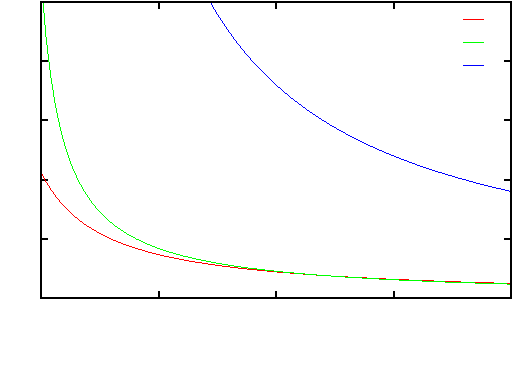
\includegraphics{nucleation_radius}}%
    \gplfronttext
  \end{picture}%
\endgroup
}\\
  \subfloat[]{\label{fig:cnt:criticalNumber}% GNUPLOT: LaTeX picture with Postscript
\begingroup
  \makeatletter
  \providecommand\color[2][]{%
    \GenericError{(gnuplot) \space\space\space\@spaces}{%
      Package color not loaded in conjunction with
      terminal option `colourtext'%
    }{See the gnuplot documentation for explanation.%
    }{Either use 'blacktext' in gnuplot or load the package
      color.sty in LaTeX.}%
    \renewcommand\color[2][]{}%
  }%
  \providecommand\includegraphics[2][]{%
    \GenericError{(gnuplot) \space\space\space\@spaces}{%
      Package graphicx or graphics not loaded%
    }{See the gnuplot documentation for explanation.%
    }{The gnuplot epslatex terminal needs graphicx.sty or graphics.sty.}%
    \renewcommand\includegraphics[2][]{}%
  }%
  \providecommand\rotatebox[2]{#2}%
  \@ifundefined{ifGPcolor}{%
    \newif\ifGPcolor
    \GPcolortrue
  }{}%
  \@ifundefined{ifGPblacktext}{%
    \newif\ifGPblacktext
    \GPblacktexttrue
  }{}%
  % define a \g@addto@macro without @ in the name:
  \let\gplgaddtomacro\g@addto@macro
  % define empty templates for all commands taking text:
  \gdef\gplbacktext{}%
  \gdef\gplfronttext{}%
  \makeatother
  \ifGPblacktext
    % no textcolor at all
    \def\colorrgb#1{}%
    \def\colorgray#1{}%
  \else
    % gray or color?
    \ifGPcolor
      \def\colorrgb#1{\color[rgb]{#1}}%
      \def\colorgray#1{\color[gray]{#1}}%
      \expandafter\def\csname LTw\endcsname{\color{white}}%
      \expandafter\def\csname LTb\endcsname{\color{black}}%
      \expandafter\def\csname LTa\endcsname{\color{black}}%
      \expandafter\def\csname LT0\endcsname{\color[rgb]{1,0,0}}%
      \expandafter\def\csname LT1\endcsname{\color[rgb]{0,1,0}}%
      \expandafter\def\csname LT2\endcsname{\color[rgb]{0,0,1}}%
      \expandafter\def\csname LT3\endcsname{\color[rgb]{1,0,1}}%
      \expandafter\def\csname LT4\endcsname{\color[rgb]{0,1,1}}%
      \expandafter\def\csname LT5\endcsname{\color[rgb]{1,1,0}}%
      \expandafter\def\csname LT6\endcsname{\color[rgb]{0,0,0}}%
      \expandafter\def\csname LT7\endcsname{\color[rgb]{1,0.3,0}}%
      \expandafter\def\csname LT8\endcsname{\color[rgb]{0.5,0.5,0.5}}%
    \else
      % gray
      \def\colorrgb#1{\color{black}}%
      \def\colorgray#1{\color[gray]{#1}}%
      \expandafter\def\csname LTw\endcsname{\color{white}}%
      \expandafter\def\csname LTb\endcsname{\color{black}}%
      \expandafter\def\csname LTa\endcsname{\color{black}}%
      \expandafter\def\csname LT0\endcsname{\color{black}}%
      \expandafter\def\csname LT1\endcsname{\color{black}}%
      \expandafter\def\csname LT2\endcsname{\color{black}}%
      \expandafter\def\csname LT3\endcsname{\color{black}}%
      \expandafter\def\csname LT4\endcsname{\color{black}}%
      \expandafter\def\csname LT5\endcsname{\color{black}}%
      \expandafter\def\csname LT6\endcsname{\color{black}}%
      \expandafter\def\csname LT7\endcsname{\color{black}}%
      \expandafter\def\csname LT8\endcsname{\color{black}}%
    \fi
  \fi
  \setlength{\unitlength}{0.0500bp}%
  \begin{picture}(5040.00,3528.00)%
    \gplgaddtomacro\gplbacktext{%
      \csname LTb\endcsname%
      \put(396,660){\makebox(0,0)[r]{\strut{} 0}}%
      \put(396,1371){\makebox(0,0)[r]{\strut{} 50}}%
      \put(396,2083){\makebox(0,0)[r]{\strut{} 100}}%
      \put(396,2794){\makebox(0,0)[r]{\strut{} 150}}%
      \put(396,3505){\makebox(0,0)[r]{\strut{} 200}}%
      \put(4908,440){\makebox(0,0){\strut{}-2}}%
      \put(3813,440){\makebox(0,0){\strut{}-1.5}}%
      \put(2718,440){\makebox(0,0){\strut{}-1}}%
      \put(1623,440){\makebox(0,0){\strut{}-0.5}}%
      \put(528,440){\makebox(0,0){\strut{} 0}}%
      \put(-374,2082){\rotatebox{90}{\makebox(0,0){\strut{}critical number of molecules}}}%
      \put(2718,110){\makebox(0,0){\strut{}negative pressure (MPa)}}%
    }%
    \gplgaddtomacro\gplfronttext{%
      \csname LTb\endcsname%
      \put(2112,1273){\makebox(0,0)[r]{\strut{}perfluorobutane}}%
      \csname LTb\endcsname%
      \put(2112,1053){\makebox(0,0)[r]{\strut{}perfluoropentane}}%
      \csname LTb\endcsname%
      \put(2112,833){\makebox(0,0)[r]{\strut{}water}}%
    }%
    \gplbacktext
    \put(0,0){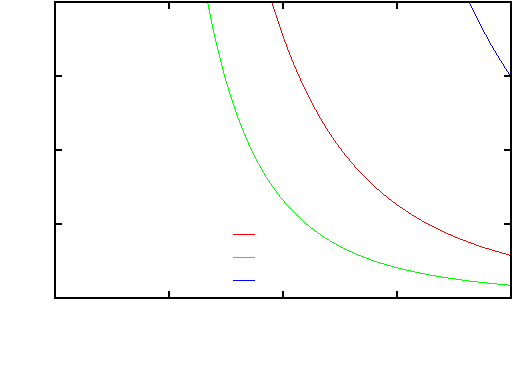
\includegraphics{nucleation_number}}%
    \gplfronttext
  \end{picture}%
\endgroup
}
\caption{
    Capillary predictions for the critical radius and critical number of molecules for a bubble as a function of the pressure at \unit{298}\kelvin.  
    The vapour is assumed to be an ideal gas, with the vapour pressure obtained by experimental fits to Antoine's equation.
    The coefficients for Antoine's equation are taken from National Institute of Standards Database\cite{NISTdata}
    (Note that the perfluorobutane data is used outside of its range of validity, see text).
  %  The other parameters are taken from the table. \tabref{nuc:parameters}.
  }
 \label{fig:cnt:nucleation_radius}
\end{figure}

We are now in a position to answer the first of our questions: the size of bubble expected to be cavitated.
This is because the critical radius provides  a lower bound for vapour bubbles in solution.
A bubble smaller than the critical radius will shrink even when  placed under tension,
and so is very unlikely to be observed.  


\figref{cnt:criticalRadius} uses equation \eqnref{LaplaceRelation} to plot the the critical radius as a function of pressure  for water, perfluoropentane and perfluorobutane
at  \unit{298}\kelvin.
The capillary approximation predicts that the critical radius is smaller for the perfluorocarbons than for water.
This is  encouraging, for it implies that type I nucleation is easier to induce for the perfluorocarbons than for water.
%However, the critical radii predicted are  somewhat large for our application.
%A \unit{20}\nano\metre-radius bubble represents more than 10\% of the radius of the oil-droplet.
%This undermines the assumption made that  neglects boundary between the oil droplet and the water.
%On the other hand, the capillary approximation is likely to be less severe.

At high pressures the critical radii of the two perfluorocarbons converge.
This is because the critical radius depends linearly on the surface tension (equation \eqnref{LaplaceRelation})
and the surface tensions are similar for perfluorocarbons.
Using a perfluorocarbon with a lower boiling point will enable smaller stable bubbles only at the more moderate  pressures where the vapour pressure plays a greater role.  
If higher pressures are used then the effect is negated.

%If therefore, Therefore, the gain in 
%At lower pressures the vapour pressure has a much greater role, which is higher in the case of perfluorobutane.
It should be noted that the vapour pressure used for perfluorobutane was extrapolated by \unit{29}\degreecelsius\  outside of its range of validity\cite{NISTdata}
 by use of Antoine's equation.
Since \unit{25}\degreecelsius\ is above the boiling point of perfluorobutane no  equilibrium vapour pressure can be defined.
However, since \unit{25}\degreecelsius\ is also well below the critical temperature, % (\tabref{:nuc:criticalTemps}), 
it is hoped that the predicted pressures within the (super-heated) bubble are still meaningful.
%The other parameters are taken from \tabref{nuc:parameters}.


In \figref{cnt:criticalNumber}  the predicted number of molecules contained within a critical bubble are plotted.
Again and as expected the number of perfluorocarbon molecules required to form a bubble are smaller than for water.
\Figref{cnt:criticalNumber} does, however, illustrate  the difficulty with the capillary approximation being used.
It is highly questionable that a bubble containing tens or even hundreds of molecules behaves like its thermodynamic bulk, with a constant density until the interface.
%The number of molecules is such that the thermodynamics starts to loose its meaning.


The capillary approximation predicts that a greater number of molecules are required to form a critical bubble for perfluorobutane than for perfluoropentane.
This is again due to the higher vapour pressure of  perfluorobutane.

%(A 20\nano\metre-diameter bubble {\em is} large to materialise by spontaneous fluctuation)
%the resulting bubble is not predicted to  contain too many molecules.
%The number of molecules within a critical bubble is perhaps more suggestive.
%This is the number of molecules that must join a bubble by fluctuation before it can grow.
%Again the number is far fewer for perfluoropentane than water.

%It is worthwhile estimating the number of molecules within the perfluoropentane bubble.
%For example, at a  negative pressure of \unit{1}\mega\pascal\ the critical radius
%of perfluoropentane is predicted to be \unit{8.7}\nano\metre\ at a vapour pressure of \unit{0.927}\ atmospheres.
%Assuming that the vapour behaves as an ideal gas, we find that the bubble contain approximately 60 molecules.




\section{Question 2: The vapourisation pressure of a perfluorocarbon droplet}\label{sec:nuc:vapourise}

There are two possible goals that may be set 
when imaging a bubble generated from a perfluorocarbon droplet:
\nlist{
 \item image the actual vaporisation event,
 \item image the resultant bubble after it has vaporised but before it redissolves.
}
%In this section we calculate the driving pressures that are required to achieve each of these goals.
Due to the stochastic nature of bubble nucleation, 
the pressures required to achieve these goals are best expressed in terms of pressures required
to achieve a given rate of nucleation,
the rate being such that observations are likely in the time frame of a given experiment.




\subsection{The rate required to image a vaporisation event}

For a nucleation event to be directly imaged
it must occur within the acoustical volume of the imaging pulse -
the volume in which the pressure is near its peak.
%
%To estimate the rate required to image a nucleation event
%we model the pulse as occupying a cylinder 
%The rate required to image a nucleation event can be estimated in terms of imaging pulse's wavelength, $\lambda$,
%and its acoustical volume, $V$.
The imaging volume is most simply approximated as a cylinder
and the pulse's principle wavelength, $\lambda$, makes a reasonable estimate for the diameter of a focused pulse.
If the pulse is $n$ cycles long then the acoustical volume, $V$, is given as so,
\begin{align}
  V \approx \frac{n  \pi \lambda^3 }{ 4}.
\end{align}
The duration of the pulse is $\tau_p=n\lambda/c$ and so it follows that the rate, $R$, at which the medium is sampled is 
\begin{align}
R \approx V/\tau_p = \frac{c\pi\lambda^2 }{4}
\label{eqn:nuc:rateOne}
\end{align}
The sampling rate of a \unit{15}\mega\hertz\ imaging pulse is therefore approximately
$\unit{10}\centi\metre\rpcubed\reciprocal\second$.
This gives the minimal rate of nucleation that would  be expected to be observed with a single a-line pulse.
It is only marginally greater than the limit of observation typically chosen in other nucleation applications: \unit{1}\centi\metre \rpcubed\reciprocal\second \cite{HongChul2005}.
For consistency with other applications, we therefore use this latter definition of  \unit{1}\centi\metre \rpcubed\reciprocal\second\
as the limit of what can be observed with ultrasound.
This corresponds to one nucleation event every 10 pulses.



\subsection{The rate required to image a generated bubble}

If only the bubble resulting from a nucleation event needs to be imaged, rather than the nucleation event itself, 
then the observable rate of nucleation is much lower.
This is because the bubble is potentially observable if the pulse passes within its lifetime 
and so it is the lifetime of the bubble, $\tau_b$, and not the duration of the acoustical pulse,
that defines the observable nucleation rate,
\begin{align}
R\approx V/\tau_b = \frac{n\pi\lambda^3}{4\tau_b}
\label{eqn:observable_rate_lifetime}
\end{align}
The value of $\tau_b$ will be evaluated when we consider the third of our questions in  \secref{nuc:lifetime}.
%To calculate the bubble's lifetime we assume that, at equilibrium, the bubble is smaller than its critical radius.
%Its lifetime is therefore defined by its rate of dissolution into the surrounding medium.
%This will be the usual case
%for although the bubble is greater than its critical radius when it is brought into existence,
%the driving wave is transient and in its absence the bubble will not normally continue to grow.



\subsection{The rate of bubble nucleation}


The rate of nucleation per unit volume is given by the Aarenhius equation, 
\begin{align}
J = J_0\exp \lr{-\frac{\Delta \Omega}{\kB T}},% = J_0 \exp\lr{- \frac{16\pi\gamma^3}{3\kB T\lr{p_v^\ast - p_L}^2}},
\label{eqn:nuc:J}
\end{align}
where $\Delta \Omega$ is the energy barrier to nucleation (in terms of the Grand Potential, $\Omega$),
$\kB$ is Boltzmann's constant, $T$ is the temperature
and $J_0$ is a rate  (per unit volume) obtained when $T\rightarrow \infty$ or when $\Delta \Omega \rightarrow 0$.

The rate constant, $J_0$, for bubble nucleation is problematic.
The reason is that the definition of a very small bubble is not clear conceptually.
What is meant, for example, by a bubble of three molecules?
And how does one know when a new molecule has joined it?
Such uncertainties mean that arguments for $J_0$ very rapidly lose their precision.
%Molecules on the bubble edge will be close to the bulk medium and so the proximity of the mo
In contradistinction, the formation of a liquid droplet from a saturated vapour is clear conceptually:
a droplet of three molecules is easy to envisage, 
a cluster of just a few molecules is easier to define than a void.
Collision theory provides plausible arguments for the rate of droplet formation in a saturated vapour\cite{Katz1973}.
%
%A collection  because the proximity of the molecules in the droplet in comparison to the vapour is what defines the droplet.
%and when a new molecule becomes associated with the droplet  for the reason 
%Despite these differences
% and how it is to be distinguished from the bulk fluid is uncertain.
% boils down to it not being clear What is meant by the rate 
Be it on the grounds of reciprocity, or simply because a better alternative cannot be found,
the rate constant $J_o$ for bubble formation is usually taken to be the same 
as that for the formation of a liquid droplet from a saturated vapour\cite{Nyquist1995}.


Rather than repeat a spurious argument we prefer to estimate $J_0$ by dimensional analysis.
The result is the same as that used in the literature and is obtained at a fraction of the effort.
In addition, the estimate obtained here does not give the impression of greater accuracy than it deserves,
a danger ever present in kinematic derivations.

%Here we argue the calculation of $J_0$ on dimensional grounds.

At high temperatures, or when the energy barrier $\Delta G$ vanishes,
one would expect the detailed chemistry of the medium to become unimportant
with the liquid medium characterised as a collection of point particles of mass, $m$, and number density, $\rho_l$.
Likewise, a vapour bubble within the medium characterised by its number density, $\rho_v$, 
and surface tension, $\gamma$.
These properties are summarised in \tabref{nuc:dimensions} along with their dimensions.
%The variables that are deemed relevant are listed in \tabref{nuc:dimensional_vars} along with their dimensions.
There are five variables listed comprising of three dimensions: mass $[M]$, length $[L]$ and time $[t]$.
It is therefore possible to write down 2 dimensionless groups\cite{Goldreich1999}.


\ctable[cap=Nucleation dimensionless groups,
        caption=Dimensionless groups in the calculation of the nucleation rate constant,
        label=table:nuc:dimensions,
        pos=top,
        %width = 0.6\textwidth,
        left
       ]
       {llcrrc}
{
}{\FL
  &        & Parameter &Symbol & Dimension & 
  \ML
  &   Bubble      &  Rate of bubble growth  & $J_0$ & $[L]^3[t]^{-1}$ &
    \NN
    &  &  Vapour number density &$\rho_v$ &  $[M][L]^{-3}$    &
    \NN
    & &   Surface tension & $\gamma$ & $[M][T]^{-2}$    &
    \ML
    &Fluid  & Fluid number density & $\rho_l$  &  $[M][L]^{-3}$   &   
    \ML
    &Particle& Particle mass & $m$ & $[M]$ &
    \LL
  }

%The 5 variables split into variables that characterise the bubble
%\nlist{
%  \item the rate of bubble growth $J_0$
%  \item the vapour mass density, $m \rho_v$,
%  \item the surface tension, $\gamma$,
%}
%and a  variable that characterise the fluid
%\nlist{
%  \item the liquid mass density, $\rho_L$.
%}

To eliminate the temporal dependence $J_0$ must be squared 
and combined with surface tension.
The resulting $J^2/\gamma$ has the units $\lrsquare{M}^{-1}\lrsquare{L}^{-6}$.
% where the square brackets denote the units of mass and length, respectively.
These dimensions can be cancelled by using the particle mass  
and the square of a number density.
There is a choice as to which of the  number densities, $\rho_L$ and  $\rho_v$,  should be used.
Le Chatelier's principle advises that that denser liquids are more expensive (in terms of energy)
to separate, and that denser bubbles are less expensive to maintain.
One would expect, therefore, the rate $J_0$ to be proportional to $\rho_v$.
%The first non-dimensional group is therefore 
\begin{align}
  \Pi_1 &= \frac{J_0^2 m}{\gamma\rho_v^2}.
 \intertext{The second dimensionless group that can then be formed is then simply ratio of the densities,}
  \Pi_2 &= \frac{\rho_v}{\rho_L}.
\end{align}
Writing $\Pi_1$ as some function, $g$, of $\Pi_2$ we obtain,
\begin{align}
   J_0 = \rho_v \sqrt{\frac{\gamma}{m}} g\lr{\frac{\rho_v}{\rho_L}}.
\end{align}
The function $g$ is undetermined but for the reasons just argued
we anticipate $g$ to increase with $\rho_v$ and decrease with $\rho_L$.
%
%If the number density of the liquid is increased above equilibrium, then the excess chemical potential will be balanced if  molecules leave the fluid and enter the bubble.
%The nucleation rate should therefore increase with $\rho_L$.
%Conversely,  the nucleation rate should  decrease with an increased vapour density, $\rho_v$.
The simplest such relationship %between rate and density 
is a linear one
and so we guess $g(x) \propto x$.
If the constant of proportionality is assumed to be approximately unity, then 
for  bubble nucleation we have
%
%This is the conventional form for the pre-exponential factor in bubble nucleation.
%
%
%The result of the collision theory argument of Katz\cite{Katz1992} is that
%%
%Due to the uncertain nature of the derivation
%Conceptually, however, bubble formation and droplet condensation are very different.
%
%However, conceptually the models are 
%The rate for a liquid droplet may be derived kinematically by  collision theory argument used to find the rate of formation of a liquid droplet from a saturated vapour.
%The adaptation is problematic, however.
%When modeIn the liquid droplet model the  droplet is modelled as a cluster of  molecules bound together, 
%and the rate   at which,  say, a fourth molecule condenses onto a cluster of three molecules is clear conceptually.
%What is meant by a `bubble of three molecules', and how it is to be distinguished from the bulk fluid is uncertain.
%Nevertheless, we use the results of such a derivation\cite{Katz1992}. % (which we provide in \appref{CNT} for completeness), 
%
%Nevertheless, we carry to calculate the rate of nucleation,
%so at least to have a benchmark with which to compare the density functional method we use in \secref{nuc:DFT}.
%
\begin{align}
  J_0 \approx \frac{\rho_v^2}{\rho_l}\sqrt{\frac{\gamma}{m}},
\end{align}
This is identical to the result of the collision theory argument of Katz\cite{Katz1992}.
%where $m$ is the mass of the particle, $rho_v$ and $\rho_l$ are the densities of the vapour and bubble respectively,
%and $\gamma$ is \todo{What is gamma}.
For water $J_0\approx 10^{34}\centi\metre \rpcubed \reciprocal\second$ and for perfluoropentane $J_0\approx 10^{32}\centi\metre \rpcubed \reciprocal\second$. 

%To complete \eqnref{observable_rate_lifetime} it is necessary to calculate the lifetime of a bubble.
%A generated bubble can either redissolve or grow and form a large bubble that will 
%float to the surface of the experimental chamber.
%Here we assume that the generated bubble is below it critical radius, 
%and we evaluate the lifetime of the bubble prior to it redissolving.



\subsection{Results}

\begin{figure}
 \centering
  \subfloat[Nucleation rates for water, \pfp\ and \pfb\ at 25\degreecelsius.]{\label{fig:cnt:rate:chem}% GNUPLOT: LaTeX picture with Postscript
\begingroup
  \makeatletter
  \providecommand\color[2][]{%
    \GenericError{(gnuplot) \space\space\space\@spaces}{%
      Package color not loaded in conjunction with
      terminal option `colourtext'%
    }{See the gnuplot documentation for explanation.%
    }{Either use 'blacktext' in gnuplot or load the package
      color.sty in LaTeX.}%
    \renewcommand\color[2][]{}%
  }%
  \providecommand\includegraphics[2][]{%
    \GenericError{(gnuplot) \space\space\space\@spaces}{%
      Package graphicx or graphics not loaded%
    }{See the gnuplot documentation for explanation.%
    }{The gnuplot epslatex terminal needs graphicx.sty or graphics.sty.}%
    \renewcommand\includegraphics[2][]{}%
  }%
  \providecommand\rotatebox[2]{#2}%
  \@ifundefined{ifGPcolor}{%
    \newif\ifGPcolor
    \GPcolortrue
  }{}%
  \@ifundefined{ifGPblacktext}{%
    \newif\ifGPblacktext
    \GPblacktexttrue
  }{}%
  % define a \g@addto@macro without @ in the name:
  \let\gplgaddtomacro\g@addto@macro
  % define empty templates for all commands taking text:
  \gdef\gplbacktext{}%
  \gdef\gplfronttext{}%
  \makeatother
  \ifGPblacktext
    % no textcolor at all
    \def\colorrgb#1{}%
    \def\colorgray#1{}%
  \else
    % gray or color?
    \ifGPcolor
      \def\colorrgb#1{\color[rgb]{#1}}%
      \def\colorgray#1{\color[gray]{#1}}%
      \expandafter\def\csname LTw\endcsname{\color{white}}%
      \expandafter\def\csname LTb\endcsname{\color{black}}%
      \expandafter\def\csname LTa\endcsname{\color{black}}%
      \expandafter\def\csname LT0\endcsname{\color[rgb]{1,0,0}}%
      \expandafter\def\csname LT1\endcsname{\color[rgb]{0,1,0}}%
      \expandafter\def\csname LT2\endcsname{\color[rgb]{0,0,1}}%
      \expandafter\def\csname LT3\endcsname{\color[rgb]{1,0,1}}%
      \expandafter\def\csname LT4\endcsname{\color[rgb]{0,1,1}}%
      \expandafter\def\csname LT5\endcsname{\color[rgb]{1,1,0}}%
      \expandafter\def\csname LT6\endcsname{\color[rgb]{0,0,0}}%
      \expandafter\def\csname LT7\endcsname{\color[rgb]{1,0.3,0}}%
      \expandafter\def\csname LT8\endcsname{\color[rgb]{0.5,0.5,0.5}}%
    \else
      % gray
      \def\colorrgb#1{\color{black}}%
      \def\colorgray#1{\color[gray]{#1}}%
      \expandafter\def\csname LTw\endcsname{\color{white}}%
      \expandafter\def\csname LTb\endcsname{\color{black}}%
      \expandafter\def\csname LTa\endcsname{\color{black}}%
      \expandafter\def\csname LT0\endcsname{\color{black}}%
      \expandafter\def\csname LT1\endcsname{\color{black}}%
      \expandafter\def\csname LT2\endcsname{\color{black}}%
      \expandafter\def\csname LT3\endcsname{\color{black}}%
      \expandafter\def\csname LT4\endcsname{\color{black}}%
      \expandafter\def\csname LT5\endcsname{\color{black}}%
      \expandafter\def\csname LT6\endcsname{\color{black}}%
      \expandafter\def\csname LT7\endcsname{\color{black}}%
      \expandafter\def\csname LT8\endcsname{\color{black}}%
    \fi
  \fi
  \setlength{\unitlength}{0.0500bp}%
  \begin{picture}(5040.00,3528.00)%
    \gplgaddtomacro\gplbacktext{%
      \csname LTb\endcsname%
      \put(1188,660){\makebox(0,0)[r]{\strut{}$10^{-40}$}}%
      \put(1188,976){\makebox(0,0)[r]{\strut{}$10^{-30}$}}%
      \put(1188,1292){\makebox(0,0)[r]{\strut{}$10^{-20}$}}%
      \put(1188,1608){\makebox(0,0)[r]{\strut{}$10^{-10}$}}%
      \put(1188,1924){\makebox(0,0)[r]{\strut{}$10^{0}$}}%
      \put(1188,2241){\makebox(0,0)[r]{\strut{}$10^{10}$}}%
      \put(1188,2557){\makebox(0,0)[r]{\strut{}$10^{20}$}}%
      \put(1188,2873){\makebox(0,0)[r]{\strut{}$10^{30}$}}%
      \put(1188,3189){\makebox(0,0)[r]{\strut{}$10^{40}$}}%
      \put(1188,3505){\makebox(0,0)[r]{\strut{}$10^{50}$}}%
      \put(4907,440){\makebox(0,0){\strut{} 1}}%
      \put(3348,440){\makebox(0,0){\strut{} 10}}%
      \put(1789,440){\makebox(0,0){\strut{} 100}}%
      \put(286,2082){\rotatebox{-270}{\makebox(0,0){\strut{}nucleation rate ($\centi\meter^{-3}\second^{-1}$)}}}%
      \put(3113,110){\makebox(0,0){\strut{}negative pressure (MPa)}}%
    }%
    \gplgaddtomacro\gplfronttext{%
      \csname LTb\endcsname%
      \put(4316,3332){\makebox(0,0)[r]{\strut{}perfluorobutane}}%
      \csname LTb\endcsname%
      \put(4316,3112){\makebox(0,0)[r]{\strut{}perfluoropentane}}%
      \csname LTb\endcsname%
      \put(4316,2892){\makebox(0,0)[r]{\strut{}water}}%
    }%
    \gplbacktext
    \put(0,0){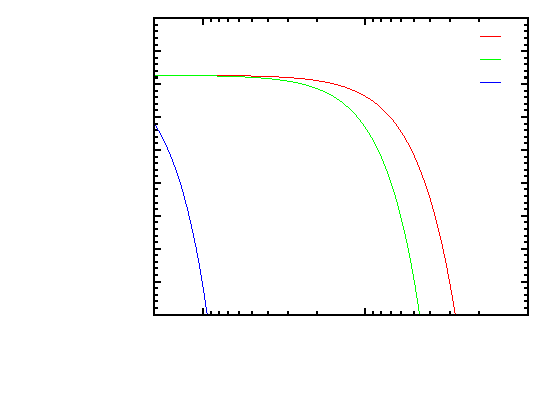
\includegraphics{c2_cnt_nucleation_rate2}}%
    \gplfronttext
  \end{picture}%
\endgroup
}\\
  \subfloat[Nucleation rates for  \pfp\ at different temperatures.]{\label{fig:cnt:rate:temp}% GNUPLOT: LaTeX picture with Postscript
\begingroup
  \makeatletter
  \providecommand\color[2][]{%
    \GenericError{(gnuplot) \space\space\space\@spaces}{%
      Package color not loaded in conjunction with
      terminal option `colourtext'%
    }{See the gnuplot documentation for explanation.%
    }{Either use 'blacktext' in gnuplot or load the package
      color.sty in LaTeX.}%
    \renewcommand\color[2][]{}%
  }%
  \providecommand\includegraphics[2][]{%
    \GenericError{(gnuplot) \space\space\space\@spaces}{%
      Package graphicx or graphics not loaded%
    }{See the gnuplot documentation for explanation.%
    }{The gnuplot epslatex terminal needs graphicx.sty or graphics.sty.}%
    \renewcommand\includegraphics[2][]{}%
  }%
  \providecommand\rotatebox[2]{#2}%
  \@ifundefined{ifGPcolor}{%
    \newif\ifGPcolor
    \GPcolortrue
  }{}%
  \@ifundefined{ifGPblacktext}{%
    \newif\ifGPblacktext
    \GPblacktexttrue
  }{}%
  % define a \g@addto@macro without @ in the name:
  \let\gplgaddtomacro\g@addto@macro
  % define empty templates for all commands taking text:
  \gdef\gplbacktext{}%
  \gdef\gplfronttext{}%
  \makeatother
  \ifGPblacktext
    % no textcolor at all
    \def\colorrgb#1{}%
    \def\colorgray#1{}%
  \else
    % gray or color?
    \ifGPcolor
      \def\colorrgb#1{\color[rgb]{#1}}%
      \def\colorgray#1{\color[gray]{#1}}%
      \expandafter\def\csname LTw\endcsname{\color{white}}%
      \expandafter\def\csname LTb\endcsname{\color{black}}%
      \expandafter\def\csname LTa\endcsname{\color{black}}%
      \expandafter\def\csname LT0\endcsname{\color[rgb]{1,0,0}}%
      \expandafter\def\csname LT1\endcsname{\color[rgb]{0,1,0}}%
      \expandafter\def\csname LT2\endcsname{\color[rgb]{0,0,1}}%
      \expandafter\def\csname LT3\endcsname{\color[rgb]{1,0,1}}%
      \expandafter\def\csname LT4\endcsname{\color[rgb]{0,1,1}}%
      \expandafter\def\csname LT5\endcsname{\color[rgb]{1,1,0}}%
      \expandafter\def\csname LT6\endcsname{\color[rgb]{0,0,0}}%
      \expandafter\def\csname LT7\endcsname{\color[rgb]{1,0.3,0}}%
      \expandafter\def\csname LT8\endcsname{\color[rgb]{0.5,0.5,0.5}}%
    \else
      % gray
      \def\colorrgb#1{\color{black}}%
      \def\colorgray#1{\color[gray]{#1}}%
      \expandafter\def\csname LTw\endcsname{\color{white}}%
      \expandafter\def\csname LTb\endcsname{\color{black}}%
      \expandafter\def\csname LTa\endcsname{\color{black}}%
      \expandafter\def\csname LT0\endcsname{\color{black}}%
      \expandafter\def\csname LT1\endcsname{\color{black}}%
      \expandafter\def\csname LT2\endcsname{\color{black}}%
      \expandafter\def\csname LT3\endcsname{\color{black}}%
      \expandafter\def\csname LT4\endcsname{\color{black}}%
      \expandafter\def\csname LT5\endcsname{\color{black}}%
      \expandafter\def\csname LT6\endcsname{\color{black}}%
      \expandafter\def\csname LT7\endcsname{\color{black}}%
      \expandafter\def\csname LT8\endcsname{\color{black}}%
    \fi
  \fi
  \setlength{\unitlength}{0.0500bp}%
  \begin{picture}(5040.00,3528.00)%
    \gplgaddtomacro\gplbacktext{%
      \csname LTb\endcsname%
      \put(1188,660){\makebox(0,0)[r]{\strut{}$10^{-40}$}}%
      \put(1188,1134){\makebox(0,0)[r]{\strut{}$10^{-30}$}}%
      \put(1188,1608){\makebox(0,0)[r]{\strut{}$10^{-20}$}}%
      \put(1188,2083){\makebox(0,0)[r]{\strut{}$10^{-10}$}}%
      \put(1188,2557){\makebox(0,0)[r]{\strut{}$10^{0}$}}%
      \put(1188,3031){\makebox(0,0)[r]{\strut{}$10^{10}$}}%
      \put(1188,3505){\makebox(0,0)[r]{\strut{}$10^{20}$}}%
      \put(4907,440){\makebox(0,0){\strut{} 1}}%
      \put(4508,440){\makebox(0,0){\strut{} 2}}%
      \put(4110,440){\makebox(0,0){\strut{} 3}}%
      \put(3711,440){\makebox(0,0){\strut{} 4}}%
      \put(3313,440){\makebox(0,0){\strut{} 5}}%
      \put(2914,440){\makebox(0,0){\strut{} 6}}%
      \put(2516,440){\makebox(0,0){\strut{} 7}}%
      \put(2117,440){\makebox(0,0){\strut{} 8}}%
      \put(1719,440){\makebox(0,0){\strut{} 9}}%
      \put(1320,440){\makebox(0,0){\strut{} 10}}%
      \put(286,2082){\rotatebox{-270}{\makebox(0,0){\strut{}nucleation rate ($\centi\meter^{-3}\second^{-1}$)}}}%
      \put(3113,110){\makebox(0,0){\strut{}negative pressure (MPa)}}%
    }%
    \gplgaddtomacro\gplfronttext{%
      \csname LTb\endcsname%
      \put(4316,3332){\makebox(0,0)[r]{\strut{}273 K}}%
      \csname LTb\endcsname%
      \put(4316,3112){\makebox(0,0)[r]{\strut{}283 K}}%
      \csname LTb\endcsname%
      \put(4316,2892){\makebox(0,0)[r]{\strut{}293 K}}%
      \csname LTb\endcsname%
      \put(4316,2672){\makebox(0,0)[r]{\strut{}303 K}}%
    }%
    \gplbacktext
    \put(0,0){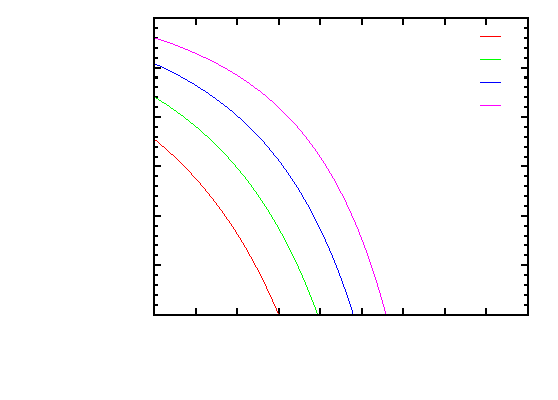
\includegraphics{c2_cnt_nucleation_rate_temp}}%
    \gplfronttext
  \end{picture}%
\endgroup
}
  \caption{
    Nucleation rates evaluated from equation \eqnref{nuc:J}.  The NIST Chemistry WebBook\cite{NISTdata} being used as the source for the required  experimental constants.
  }
 \label{fig:cnt:rate}
\end{figure}


The nucleation rates calculated with the capillary approximation are plotted in \figref{cnt:rate}.
In \figref{cnt:rate:chem} the rates   for \pfb,  perfluoropentane and water are plotted.
As expected from the plot of critical radii, \figref{cnt:criticalRadius}, 
high rates of nucleation are obtained at lower pressures with the perflurocarbons than for water,
with \pfb\ being more easily cavitated than \pfp.
This is encouraging, for increasing the rate of type I nucleation was the motivation for considering the perfluorocarbons.


However, the pressures given by \figref{cnt:rate}  to observe type I nucleation are high for diagnostic ultrasound.
\figref{cnt:rate:chem} suggests that  \pfb, even when in a supersaturated state,
will  require a negative pressure in the region of \unit{4}\mega\pascal\ to be observable. 
Such pressures are used in medical ultrasound, but require the specially engineered transducers of HIFU.
To observe \pfp\ the negative pressure will need to be in the region of \unit{8}\mega\pascal,
and while \figref{cnt:rate:temp} shows that the temperature is influential, 
it is not so influential as to shift the pressures back to those obtainable with diagnostic transducers.
These pressures are of the same order of magnitude as the experimental values of Schad\cite{Schad2009}.




\section{Question 3: The lifetime of a vapour bubble}\label{sec:nuc:lifetime}


\begin{figure}
  \hspace*{-20mm}
  \subfloat[Dissolution of a \unit{1}\micro\metre\ air bubble when $\zeta=0$]{ \label{fig:nuc:dissolve_time_lum}% GNUPLOT: LaTeX picture with Postscript
\begingroup
  \makeatletter
  \providecommand\color[2][]{%
    \GenericError{(gnuplot) \space\space\space\@spaces}{%
      Package color not loaded in conjunction with
      terminal option `colourtext'%
    }{See the gnuplot documentation for explanation.%
    }{Either use 'blacktext' in gnuplot or load the package
      color.sty in LaTeX.}%
    \renewcommand\color[2][]{}%
  }%
  \providecommand\includegraphics[2][]{%
    \GenericError{(gnuplot) \space\space\space\@spaces}{%
      Package graphicx or graphics not loaded%
    }{See the gnuplot documentation for explanation.%
    }{The gnuplot epslatex terminal needs graphicx.sty or graphics.sty.}%
    \renewcommand\includegraphics[2][]{}%
  }%
  \providecommand\rotatebox[2]{#2}%
  \@ifundefined{ifGPcolor}{%
    \newif\ifGPcolor
    \GPcolorfalse
  }{}%
  \@ifundefined{ifGPblacktext}{%
    \newif\ifGPblacktext
    \GPblacktexttrue
  }{}%
  % define a \g@addto@macro without @ in the name:
  \let\gplgaddtomacro\g@addto@macro
  % define empty templates for all commands taking text:
  \gdef\gplbacktext{}%
  \gdef\gplfronttext{}%
  \makeatother
  \ifGPblacktext
    % no textcolor at all
    \def\colorrgb#1{}%
    \def\colorgray#1{}%
  \else
    % gray or color?
    \ifGPcolor
      \def\colorrgb#1{\color[rgb]{#1}}%
      \def\colorgray#1{\color[gray]{#1}}%
      \expandafter\def\csname LTw\endcsname{\color{white}}%
      \expandafter\def\csname LTb\endcsname{\color{black}}%
      \expandafter\def\csname LTa\endcsname{\color{black}}%
      \expandafter\def\csname LT0\endcsname{\color[rgb]{1,0,0}}%
      \expandafter\def\csname LT1\endcsname{\color[rgb]{0,1,0}}%
      \expandafter\def\csname LT2\endcsname{\color[rgb]{0,0,1}}%
      \expandafter\def\csname LT3\endcsname{\color[rgb]{1,0,1}}%
      \expandafter\def\csname LT4\endcsname{\color[rgb]{0,1,1}}%
      \expandafter\def\csname LT5\endcsname{\color[rgb]{1,1,0}}%
      \expandafter\def\csname LT6\endcsname{\color[rgb]{0,0,0}}%
      \expandafter\def\csname LT7\endcsname{\color[rgb]{1,0.3,0}}%
      \expandafter\def\csname LT8\endcsname{\color[rgb]{0.5,0.5,0.5}}%
    \else
      % gray
      \def\colorrgb#1{\color{black}}%
      \def\colorgray#1{\color[gray]{#1}}%
      \expandafter\def\csname LTw\endcsname{\color{white}}%
      \expandafter\def\csname LTb\endcsname{\color{black}}%
      \expandafter\def\csname LTa\endcsname{\color{black}}%
      \expandafter\def\csname LT0\endcsname{\color{black}}%
      \expandafter\def\csname LT1\endcsname{\color{black}}%
      \expandafter\def\csname LT2\endcsname{\color{black}}%
      \expandafter\def\csname LT3\endcsname{\color{black}}%
      \expandafter\def\csname LT4\endcsname{\color{black}}%
      \expandafter\def\csname LT5\endcsname{\color{black}}%
      \expandafter\def\csname LT6\endcsname{\color{black}}%
      \expandafter\def\csname LT7\endcsname{\color{black}}%
      \expandafter\def\csname LT8\endcsname{\color{black}}%
    \fi
  \fi
  \setlength{\unitlength}{0.0500bp}%
  \begin{picture}(4320.00,3024.00)%
    \gplgaddtomacro\gplbacktext{%
      \csname LTb\endcsname%
      \put(946,704){\makebox(0,0)[r]{\strut{} 0}}%
      \put(946,910){\makebox(0,0)[r]{\strut{} 0.1}}%
      \put(946,1115){\makebox(0,0)[r]{\strut{} 0.2}}%
      \put(946,1321){\makebox(0,0)[r]{\strut{} 0.3}}%
      \put(946,1526){\makebox(0,0)[r]{\strut{} 0.4}}%
      \put(946,1732){\makebox(0,0)[r]{\strut{} 0.5}}%
      \put(946,1937){\makebox(0,0)[r]{\strut{} 0.6}}%
      \put(946,2143){\makebox(0,0)[r]{\strut{} 0.7}}%
      \put(946,2348){\makebox(0,0)[r]{\strut{} 0.8}}%
      \put(946,2554){\makebox(0,0)[r]{\strut{} 0.9}}%
      \put(946,2759){\makebox(0,0)[r]{\strut{} 1}}%
      \put(1078,484){\makebox(0,0){\strut{} 0}}%
      \put(1434,484){\makebox(0,0){\strut{} 2}}%
      \put(1789,484){\makebox(0,0){\strut{} 4}}%
      \put(2145,484){\makebox(0,0){\strut{} 6}}%
      \put(2501,484){\makebox(0,0){\strut{} 8}}%
      \put(2856,484){\makebox(0,0){\strut{} 10}}%
      \put(3212,484){\makebox(0,0){\strut{} 12}}%
      \put(3567,484){\makebox(0,0){\strut{} 14}}%
      \put(3923,484){\makebox(0,0){\strut{} 16}}%
      \put(176,1731){\rotatebox{-270}{\makebox(0,0){\strut{}radius ($\mu$m)}}}%
      \put(2500,154){\makebox(0,0){\strut{}time (ms)}}%
    }%
    \gplgaddtomacro\gplfronttext{%
    }%
    \gplbacktext
    \put(0,0){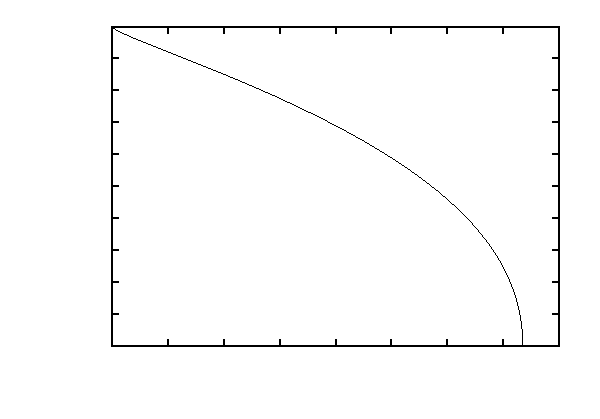
\includegraphics{chNucDissolveTimeLum}}%
    \gplfronttext
  \end{picture}%
\endgroup
}
  \subfloat[Dissolution time as a function of radius]{ \label{fig:nuc:dissolve_time}% GNUPLOT: LaTeX picture with Postscript
\begingroup
  \makeatletter
  \providecommand\color[2][]{%
    \GenericError{(gnuplot) \space\space\space\@spaces}{%
      Package color not loaded in conjunction with
      terminal option `colourtext'%
    }{See the gnuplot documentation for explanation.%
    }{Either use 'blacktext' in gnuplot or load the package
      color.sty in LaTeX.}%
    \renewcommand\color[2][]{}%
  }%
  \providecommand\includegraphics[2][]{%
    \GenericError{(gnuplot) \space\space\space\@spaces}{%
      Package graphicx or graphics not loaded%
    }{See the gnuplot documentation for explanation.%
    }{The gnuplot epslatex terminal needs graphicx.sty or graphics.sty.}%
    \renewcommand\includegraphics[2][]{}%
  }%
  \providecommand\rotatebox[2]{#2}%
  \@ifundefined{ifGPcolor}{%
    \newif\ifGPcolor
    \GPcolorfalse
  }{}%
  \@ifundefined{ifGPblacktext}{%
    \newif\ifGPblacktext
    \GPblacktexttrue
  }{}%
  % define a \g@addto@macro without @ in the name:
  \let\gplgaddtomacro\g@addto@macro
  % define empty templates for all commands taking text:
  \gdef\gplbacktext{}%
  \gdef\gplfronttext{}%
  \makeatother
  \ifGPblacktext
    % no textcolor at all
    \def\colorrgb#1{}%
    \def\colorgray#1{}%
  \else
    % gray or color?
    \ifGPcolor
      \def\colorrgb#1{\color[rgb]{#1}}%
      \def\colorgray#1{\color[gray]{#1}}%
      \expandafter\def\csname LTw\endcsname{\color{white}}%
      \expandafter\def\csname LTb\endcsname{\color{black}}%
      \expandafter\def\csname LTa\endcsname{\color{black}}%
      \expandafter\def\csname LT0\endcsname{\color[rgb]{1,0,0}}%
      \expandafter\def\csname LT1\endcsname{\color[rgb]{0,1,0}}%
      \expandafter\def\csname LT2\endcsname{\color[rgb]{0,0,1}}%
      \expandafter\def\csname LT3\endcsname{\color[rgb]{1,0,1}}%
      \expandafter\def\csname LT4\endcsname{\color[rgb]{0,1,1}}%
      \expandafter\def\csname LT5\endcsname{\color[rgb]{1,1,0}}%
      \expandafter\def\csname LT6\endcsname{\color[rgb]{0,0,0}}%
      \expandafter\def\csname LT7\endcsname{\color[rgb]{1,0.3,0}}%
      \expandafter\def\csname LT8\endcsname{\color[rgb]{0.5,0.5,0.5}}%
    \else
      % gray
      \def\colorrgb#1{\color{black}}%
      \def\colorgray#1{\color[gray]{#1}}%
      \expandafter\def\csname LTw\endcsname{\color{white}}%
      \expandafter\def\csname LTb\endcsname{\color{black}}%
      \expandafter\def\csname LTa\endcsname{\color{black}}%
      \expandafter\def\csname LT0\endcsname{\color{black}}%
      \expandafter\def\csname LT1\endcsname{\color{black}}%
      \expandafter\def\csname LT2\endcsname{\color{black}}%
      \expandafter\def\csname LT3\endcsname{\color{black}}%
      \expandafter\def\csname LT4\endcsname{\color{black}}%
      \expandafter\def\csname LT5\endcsname{\color{black}}%
      \expandafter\def\csname LT6\endcsname{\color{black}}%
      \expandafter\def\csname LT7\endcsname{\color{black}}%
      \expandafter\def\csname LT8\endcsname{\color{black}}%
    \fi
  \fi
  \setlength{\unitlength}{0.0500bp}%
  \begin{picture}(4320.00,3024.00)%
    \gplgaddtomacro\gplbacktext{%
      \csname LTb\endcsname%
      \put(946,704){\makebox(0,0)[r]{\strut{}$10^{-2}$}}%
      \put(946,1115){\makebox(0,0)[r]{\strut{}$10^{-1}$}}%
      \put(946,1526){\makebox(0,0)[r]{\strut{}$10^{0}$}}%
      \put(946,1937){\makebox(0,0)[r]{\strut{}$10^{1}$}}%
      \put(946,2348){\makebox(0,0)[r]{\strut{}$10^{2}$}}%
      \put(946,2759){\makebox(0,0)[r]{\strut{}$10^{3}$}}%
      \put(1078,484){\makebox(0,0){\strut{}$10^{-2}$}}%
      \put(2026,484){\makebox(0,0){\strut{}$10^{-1}$}}%
      \put(2975,484){\makebox(0,0){\strut{}$10^{0}$}}%
      \put(3923,484){\makebox(0,0){\strut{}$10^{1}$}}%
      \put(176,1731){\rotatebox{-270}{\makebox(0,0){\strut{}dissolution time (ms)}}}%
      \put(2500,154){\makebox(0,0){\strut{}initial radius ($\mu$m)}}%
    }%
    \gplgaddtomacro\gplfronttext{%
      \csname LTb\endcsname%
      \put(2662,2586){\makebox(0,0)[r]{\strut{}saturated}}%
      \csname LTb\endcsname%
      \put(2662,2366){\makebox(0,0)[r]{\strut{}unsaturated}}%
    }%
    \gplbacktext
    \put(0,0){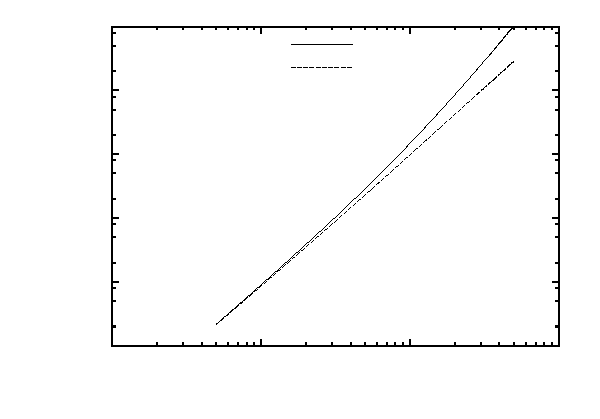
\includegraphics{chNucDissolveTime}}%
    \gplfronttext
  \end{picture}%
\endgroup
}
  \caption{ Dissolve times of air bubbles.  The experimental quantities used in the model are given in \tabref{nuc:dissolveVars}.}
\end{figure}

\begin{figure}
  \hspace*{-20mm}
  \subfloat[Dissolution of a \unit{1}\micro\metre\ \pfp\ bubble when $\zeta=0$]{\label{fig:nuc:dissolve_time_lumPFP}% GNUPLOT: LaTeX picture with Postscript
\begingroup
  \makeatletter
  \providecommand\color[2][]{%
    \GenericError{(gnuplot) \space\space\space\@spaces}{%
      Package color not loaded in conjunction with
      terminal option `colourtext'%
    }{See the gnuplot documentation for explanation.%
    }{Either use 'blacktext' in gnuplot or load the package
      color.sty in LaTeX.}%
    \renewcommand\color[2][]{}%
  }%
  \providecommand\includegraphics[2][]{%
    \GenericError{(gnuplot) \space\space\space\@spaces}{%
      Package graphicx or graphics not loaded%
    }{See the gnuplot documentation for explanation.%
    }{The gnuplot epslatex terminal needs graphicx.sty or graphics.sty.}%
    \renewcommand\includegraphics[2][]{}%
  }%
  \providecommand\rotatebox[2]{#2}%
  \@ifundefined{ifGPcolor}{%
    \newif\ifGPcolor
    \GPcolorfalse
  }{}%
  \@ifundefined{ifGPblacktext}{%
    \newif\ifGPblacktext
    \GPblacktexttrue
  }{}%
  % define a \g@addto@macro without @ in the name:
  \let\gplgaddtomacro\g@addto@macro
  % define empty templates for all commands taking text:
  \gdef\gplbacktext{}%
  \gdef\gplfronttext{}%
  \makeatother
  \ifGPblacktext
    % no textcolor at all
    \def\colorrgb#1{}%
    \def\colorgray#1{}%
  \else
    % gray or color?
    \ifGPcolor
      \def\colorrgb#1{\color[rgb]{#1}}%
      \def\colorgray#1{\color[gray]{#1}}%
      \expandafter\def\csname LTw\endcsname{\color{white}}%
      \expandafter\def\csname LTb\endcsname{\color{black}}%
      \expandafter\def\csname LTa\endcsname{\color{black}}%
      \expandafter\def\csname LT0\endcsname{\color[rgb]{1,0,0}}%
      \expandafter\def\csname LT1\endcsname{\color[rgb]{0,1,0}}%
      \expandafter\def\csname LT2\endcsname{\color[rgb]{0,0,1}}%
      \expandafter\def\csname LT3\endcsname{\color[rgb]{1,0,1}}%
      \expandafter\def\csname LT4\endcsname{\color[rgb]{0,1,1}}%
      \expandafter\def\csname LT5\endcsname{\color[rgb]{1,1,0}}%
      \expandafter\def\csname LT6\endcsname{\color[rgb]{0,0,0}}%
      \expandafter\def\csname LT7\endcsname{\color[rgb]{1,0.3,0}}%
      \expandafter\def\csname LT8\endcsname{\color[rgb]{0.5,0.5,0.5}}%
    \else
      % gray
      \def\colorrgb#1{\color{black}}%
      \def\colorgray#1{\color[gray]{#1}}%
      \expandafter\def\csname LTw\endcsname{\color{white}}%
      \expandafter\def\csname LTb\endcsname{\color{black}}%
      \expandafter\def\csname LTa\endcsname{\color{black}}%
      \expandafter\def\csname LT0\endcsname{\color{black}}%
      \expandafter\def\csname LT1\endcsname{\color{black}}%
      \expandafter\def\csname LT2\endcsname{\color{black}}%
      \expandafter\def\csname LT3\endcsname{\color{black}}%
      \expandafter\def\csname LT4\endcsname{\color{black}}%
      \expandafter\def\csname LT5\endcsname{\color{black}}%
      \expandafter\def\csname LT6\endcsname{\color{black}}%
      \expandafter\def\csname LT7\endcsname{\color{black}}%
      \expandafter\def\csname LT8\endcsname{\color{black}}%
    \fi
  \fi
  \setlength{\unitlength}{0.0500bp}%
  \begin{picture}(5760.00,4032.00)%
    \gplgaddtomacro\gplbacktext{%
      \csname LTb\endcsname%
      \put(946,704){\makebox(0,0)[r]{\strut{} 0}}%
      \put(946,1010){\makebox(0,0)[r]{\strut{} 0.1}}%
      \put(946,1317){\makebox(0,0)[r]{\strut{} 0.2}}%
      \put(946,1623){\makebox(0,0)[r]{\strut{} 0.3}}%
      \put(946,1929){\makebox(0,0)[r]{\strut{} 0.4}}%
      \put(946,2236){\makebox(0,0)[r]{\strut{} 0.5}}%
      \put(946,2542){\makebox(0,0)[r]{\strut{} 0.6}}%
      \put(946,2848){\makebox(0,0)[r]{\strut{} 0.7}}%
      \put(946,3154){\makebox(0,0)[r]{\strut{} 0.8}}%
      \put(946,3461){\makebox(0,0)[r]{\strut{} 0.9}}%
      \put(946,3767){\makebox(0,0)[r]{\strut{} 1}}%
      \put(1078,484){\makebox(0,0){\strut{} 0}}%
      \put(1792,484){\makebox(0,0){\strut{} 20}}%
      \put(2506,484){\makebox(0,0){\strut{} 40}}%
      \put(3221,484){\makebox(0,0){\strut{} 60}}%
      \put(3935,484){\makebox(0,0){\strut{} 80}}%
      \put(4649,484){\makebox(0,0){\strut{} 100}}%
      \put(5363,484){\makebox(0,0){\strut{} 120}}%
      \put(176,2235){\rotatebox{-270}{\makebox(0,0){\strut{}radius ($\mu$m)}}}%
      \put(3220,154){\makebox(0,0){\strut{}time (s)}}%
    }%
    \gplgaddtomacro\gplfronttext{%
    }%
    \gplbacktext
    \put(0,0){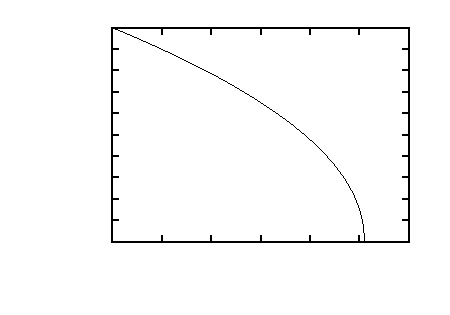
\includegraphics{chNucDissolveTimeLumPFP}}%
    \gplfronttext
  \end{picture}%
\endgroup
}
  \subfloat[Dissolution time as a function of radius]{\label{fig:nuc:dissolve_timePFP}% GNUPLOT: LaTeX picture with Postscript
\begingroup
  \makeatletter
  \providecommand\color[2][]{%
    \GenericError{(gnuplot) \space\space\space\@spaces}{%
      Package color not loaded in conjunction with
      terminal option `colourtext'%
    }{See the gnuplot documentation for explanation.%
    }{Either use 'blacktext' in gnuplot or load the package
      color.sty in LaTeX.}%
    \renewcommand\color[2][]{}%
  }%
  \providecommand\includegraphics[2][]{%
    \GenericError{(gnuplot) \space\space\space\@spaces}{%
      Package graphicx or graphics not loaded%
    }{See the gnuplot documentation for explanation.%
    }{The gnuplot epslatex terminal needs graphicx.sty or graphics.sty.}%
    \renewcommand\includegraphics[2][]{}%
  }%
  \providecommand\rotatebox[2]{#2}%
  \@ifundefined{ifGPcolor}{%
    \newif\ifGPcolor
    \GPcolorfalse
  }{}%
  \@ifundefined{ifGPblacktext}{%
    \newif\ifGPblacktext
    \GPblacktexttrue
  }{}%
  % define a \g@addto@macro without @ in the name:
  \let\gplgaddtomacro\g@addto@macro
  % define empty templates for all commands taking text:
  \gdef\gplbacktext{}%
  \gdef\gplfronttext{}%
  \makeatother
  \ifGPblacktext
    % no textcolor at all
    \def\colorrgb#1{}%
    \def\colorgray#1{}%
  \else
    % gray or color?
    \ifGPcolor
      \def\colorrgb#1{\color[rgb]{#1}}%
      \def\colorgray#1{\color[gray]{#1}}%
      \expandafter\def\csname LTw\endcsname{\color{white}}%
      \expandafter\def\csname LTb\endcsname{\color{black}}%
      \expandafter\def\csname LTa\endcsname{\color{black}}%
      \expandafter\def\csname LT0\endcsname{\color[rgb]{1,0,0}}%
      \expandafter\def\csname LT1\endcsname{\color[rgb]{0,1,0}}%
      \expandafter\def\csname LT2\endcsname{\color[rgb]{0,0,1}}%
      \expandafter\def\csname LT3\endcsname{\color[rgb]{1,0,1}}%
      \expandafter\def\csname LT4\endcsname{\color[rgb]{0,1,1}}%
      \expandafter\def\csname LT5\endcsname{\color[rgb]{1,1,0}}%
      \expandafter\def\csname LT6\endcsname{\color[rgb]{0,0,0}}%
      \expandafter\def\csname LT7\endcsname{\color[rgb]{1,0.3,0}}%
      \expandafter\def\csname LT8\endcsname{\color[rgb]{0.5,0.5,0.5}}%
    \else
      % gray
      \def\colorrgb#1{\color{black}}%
      \def\colorgray#1{\color[gray]{#1}}%
      \expandafter\def\csname LTw\endcsname{\color{white}}%
      \expandafter\def\csname LTb\endcsname{\color{black}}%
      \expandafter\def\csname LTa\endcsname{\color{black}}%
      \expandafter\def\csname LT0\endcsname{\color{black}}%
      \expandafter\def\csname LT1\endcsname{\color{black}}%
      \expandafter\def\csname LT2\endcsname{\color{black}}%
      \expandafter\def\csname LT3\endcsname{\color{black}}%
      \expandafter\def\csname LT4\endcsname{\color{black}}%
      \expandafter\def\csname LT5\endcsname{\color{black}}%
      \expandafter\def\csname LT6\endcsname{\color{black}}%
      \expandafter\def\csname LT7\endcsname{\color{black}}%
      \expandafter\def\csname LT8\endcsname{\color{black}}%
    \fi
  \fi
  \setlength{\unitlength}{0.0500bp}%
  \begin{picture}(4320.00,3024.00)%
    \gplgaddtomacro\gplbacktext{%
      \csname LTb\endcsname%
      \put(946,704){\makebox(0,0)[r]{\strut{}$10^{-1}$}}%
      \put(946,1047){\makebox(0,0)[r]{\strut{}$10^{0}$}}%
      \put(946,1389){\makebox(0,0)[r]{\strut{}$10^{1}$}}%
      \put(946,1732){\makebox(0,0)[r]{\strut{}$10^{2}$}}%
      \put(946,2074){\makebox(0,0)[r]{\strut{}$10^{3}$}}%
      \put(946,2417){\makebox(0,0)[r]{\strut{}$10^{4}$}}%
      \put(946,2759){\makebox(0,0)[r]{\strut{}$10^{5}$}}%
      \put(1078,484){\makebox(0,0){\strut{}$10^{-2}$}}%
      \put(2026,484){\makebox(0,0){\strut{}$10^{-1}$}}%
      \put(2975,484){\makebox(0,0){\strut{}$10^{0}$}}%
      \put(3923,484){\makebox(0,0){\strut{}$10^{1}$}}%
      \put(176,1731){\rotatebox{-270}{\makebox(0,0){\strut{}dissolution time (s)}}}%
      \put(2500,154){\makebox(0,0){\strut{}initial radius ($\mu$m)}}%
    }%
    \gplgaddtomacro\gplfronttext{%
      \csname LTb\endcsname%
      \put(2662,2586){\makebox(0,0)[r]{\strut{}saturated}}%
      \csname LTb\endcsname%
      \put(2662,2366){\makebox(0,0)[r]{\strut{}unsaturated}}%
    }%
    \gplbacktext
    \put(0,0){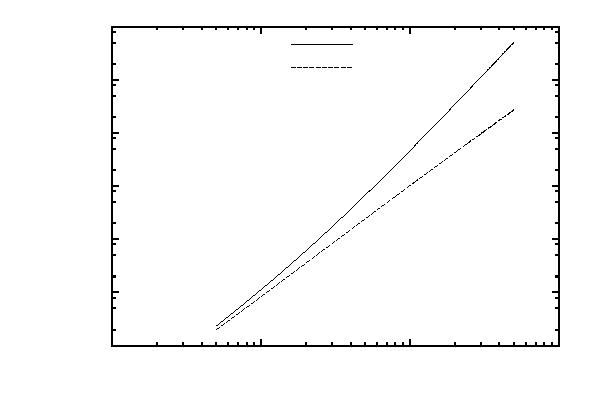
\includegraphics{chNucDissolveTimePFP}}%
    \gplfronttext
  \end{picture}%
\endgroup
}
  \caption{ Dissolve times of \pfp\ bubbles.  The experimental quantities used in the model are given in \tabref{nuc:dissolveVars}. }
 \label{fig:nuc:dissolve_time_lum}
\end{figure}

%\resizebox{\columnwidth}{!}{%
\ctable[cap=Dissolution symbols,
        caption=Symbols used in the calculation of dissolution times,
        label=table:nuc:dissolveVars,
        pos=top,
        doinside=\small\hspace*{-0mm},
        width = 0.99\textwidth,
        left
       ]
       {llllrrc}
{\tnote{Estimated with the Hayduk-Laudie equation}
}{\FL
  &   Symbol     & Description & units &Value (Air) & Value (PFP) & 
  \ML
    &$\gamma$ &   Surface tension &$\newton/\metre$ &  ${0.07280}$ \cite{Sarkar2009}   & ${0.0096828}$ \cite{NISTdata}    &
    \ML
   % &H  & Henry's constant & ${\{1.48472\times 10^{-7}} \metre^2 \kilo\gram \second^{-2} \mole^{-1}$\cite{Sarkar2009}  &  $ {3.54634\times 10^{-4}} \metre^2 \kilo\gram \second^{-2} \mole^{-1}$\cite{CASPFP}   &  
    &$H$ & Henry's constant   &$\metre^2 \kilo\gram \second^{-2} \mole^{-1}$ &  ${1.48472\times 10^{-7}} $\cite{Sarkar2009}   &  $ {3.54634\times 10^{-4}}$\cite{CASPFP}     &
    \ML
    &$D$ & Diffusivity   &$\metre^2 \second^{-1} $ &  ${2.05\times 10^{-9}} $\cite{Sarkar2009}   &  $ {6.409\times 10^{-10}}$\tmark     &
 %   &H  & Henry's constant &   &   &  
   \ML
   &$P_\infty$&  Ambient Pressure & $\mega\pascal$ & ${0.101325}$ &${0.101325}$ &
    \LL
  }
%}

The third and final question of this chapter regards the expected lifetime of a bubble.
In \secref{nuc:evacuate} the critical radius was used to give a lower bound on the size of a 
bubble generated in a perfluorocarbon droplet or evacuated from a mote.
It was seen that bubbles in the tens of nanometres can be stable when placed under 
tension by the rarefactional cycles of an acoustic field.
The expected lifetime of the bubble after the rarefaction has passed will now be calculated.

This section uses a very simple model that was first derived by Epstein and Plesset\cite{Epstein1950},
although we prefer the notation of Gor\cite{Gor2011}.
The hope is to obtain only an order of magnitude estimate of the bubble lifetime
and so some accuracy can be foregone.

In the model a gas bubble is placed in a fluid of uniform pressure,
where the medium in the vicinity of the bubble contains the gas at concentration $n_o$.
Two gas bubbles will be considered, 
an air bubble that contains nitrogen and oxygen,
and a perfluoropentane bubble.
In each case it will be assumed that the bubble contains no water vapour,
and that the surface of the bubble is has no stabilising shell\footnote{%
See Sarkar\cite{Sarkar2009} for a recent discussion of the dissolution of a bubble that has  a permeable shell.%
}.
The concentration of the medium far from the bubble is denoted $n_\infty$
and is chosen to be the ambient density of the gas in the medium at standard temperature, $T$, and pressure, $p_\infty$.
While we imagine the bubble to be generated in a rarefaction cycle of an acoustic wave
we neither model the generation of the bubble nor the sound pulse.


There are two cases of particular interest
\nlist{
\item
  when the concentration of dissolved gas in the bubble's vicinity  is equal to the ambient concentration,
   \begin{align}
    n_0 &= n_\infty.
  \end{align}
  Such will be the case when a bubble in generated in a medium that is unaltered by the passing of the acoustic wave.
  This will typically be the case for short pulses of low pressure.
\item 
  when the concentration of the gas in the bubble's vicinity is much lower than the ambient concentration. 
  This situation can arise when a previous pulse of a high pressure wave has already evacuated most of the gas in the focal zone.
  The limiting case is when 
   \begin{align}
    n_0 &= 0.
  \end{align}
}
It is therefore natural to frame the derivation in terms a dimensionless measure of saturation,
\begin{align}
  \zeta &\equiv \frac{n_0 - n_\infty}{n_\infty }\label{eqn:nuc:saturation}
\end{align}
The two cases of interest are  when $\zeta = 0$ and $\zeta = -1$.
The solubility of the medium will make a second useful dimensionless quantity\cite{Gor2011}
\begin{align}
  s &\equiv \frac{\kB T n_\infty}{P_\infty} \label{eqn:nuc:solubility}.
\end{align}

Imbalances in the number density of the gas in the medium will prompt diffusion from the vicinity of the bubble to the bulk.
Modelling this as Fickian diffusion  in a spherical geometry gives,
\begin{align}
  j_D = -D \frac{\partial n}{\partial r}
  \label{eqn:nuc:Fickian}
\end{align}
where  the density is a spherical symmetric function of radius, $r$.
If diffusion transport terms are neglected then \eqnref{nuc:Fickian} can be solved to obtain,
\begin{align}
  \frac{\partial n}{\partial r} = \lr{n_R - n_0}\lrsquare{\frac{1}{R} + \frac{1}{\sqrt{\pi D t}}},
\end{align}
where $R$ is the bubble radius and $n_R$ is the concentration of dissolved gas at that radius.
The details of the derivation were given in Epstein and Plesset's \cite{Epstein1950} original paper and do not need to be reproduced here.

Material conservation requires that the number of particles passing through the radius of the bubble
equates to the change in the number of particles in the bubble, $N$,
\begin{align}
  \frac{dN}{dt} =4 \pi R^2 D\frac{\partial n}{\partial r}.
\label{eqn:nuc:materialCons}
\end{align}

Modelling the contents of the bubble as an ideal gas lets the particle number be expressed in terms of the ambient pressure, $P_\infty$, and surface tension $\gamma$ of the bubble,
\begin{align}
  N = \frac{4\pi R^3 }{3\kB T} \lrsquare{P_\infty + \frac{2\gamma}{R}}.
  \label{eqn:nuc:ParticleNumber}
\end{align}
By differentiating \eqnref{nuc:ParticleNumber} and equating the result to \eqnref{nuc:materialCons} a differential equation for the change in bubble radius is obtained,
\begin{align}
   \dot{R}\lrsquare{ 1+ \frac{4\gamma}{3 P_\infty R}} = Ds\lrsquare{ \zeta - \frac{2\gamma}{P_\infty R}}\lrsquare{\frac{1}{R} + \frac{1}{\sqrt{\pi D t}}},
   \label{eqn:nuc:Rdot}
\end{align}
where equation \eqnref{nuc:solubility} has been used, along with
\begin{align}
  \frac{\lr{n_0 - n_R}}{n_\infty} = \zeta - \frac{2\gamma}{P_\infty R}
  \label{eqn:nuc:dissolve}
\end{align}
which follows from \eqnref{nuc:saturation}.






The numerical solution of \eqnref{nuc:Rdot} is plotted for a 1 micron air bubble in \figref{nuc:dissolve_time_lum}.
It is seen that the bubble radius decreases fairly constantly until a very rapid final collapse.
The lack of a long tail in \figref{nuc:dissolve_time_lum}
means that the dissolution time is dominated by periods when the bubble is near is starting radius.
There is not a long decay during which the bubble is technically existent but is so small as to be unobservable.

The dissolution time for an air bubble as a function of radius is plotted in \figref{nuc:dissolve_time}.
Both the saturated and unsaturated cases are plotted.
The dissolution times for very small bubbles is very similar,
but starts to diverge for bubbles of radius \unit{0.5}\micro\metre.

The lifetime of a free submicron air bubble is of order \unit{1}\milli\second\ in both the  saturated and unsaturated cases.
The pulse duration of diagnostic ultrasound is typically measured in microseconds and so the bubble would be expected to live throughout the duration of the pulse.
However, adjacent alines in a diagnostic pulse are often tens of milliseconds apart.
Submicron air bubbles would not be expected to exist in adjacent alines.
The short lifetimes of air bubbles mean that care needs to be taken to synchronise the generation and the imaging of a bubble,
so that the imaging wave samples the same focal region as the driving wave within a few microseconds of the driving wave passing.
%In this case the observable rate of nucleation given is given by equation \eqnref{nuc:rateOne}.


The solubility of the perfluorocarbons in water is much lower than for nitrogen and oxygen.
While the dissolution characteristics are very similar to an air bubble (\figref{nuc:dissolve_timePFP})
the timescale for dissolution is order of magnitudes larger (\figref{nuc:dissolve_time_lumPFP}).
This has the advantage that a bubble can be generated at a different time (and therefore at a different location)
to where the bubble is imaged.
In this case  the driving wave and the imaging wave can be considered independently.

\section{Discussion}\label{sec:nuc:discussion}

\subsection{Summary of results}

In this chapter the two broad approaches of generating a bubble with sound for the purpose of imaging are analysed.

On the one hand one may attempt to create a bubble via type I nucleation.
The pressures required to do so in water are beyond the capabilities of diagnostic ultrasound
and so one may instead focus on creating an emulsion with a second medium that is easier to nucleate.
The perfluorocarbons, due to their low boiling points, low solubility and low toxicity make excellent 
candidates.
This chapter has suggested by means of the capillary approximation that very few perfluoro-molecules are 
needed to create a bubble, and that the nucleating pressure is much reduced - down to \unit{7-8}\mega\pascal\ negative pressure for
perfluoropentane
These pressures are still on the cusp of what is used in medical ultrasound
and are still beyond what can be achieved with a diagnostic transducer.
However, given the questions regarding the approximation's accuracy that are raised by the calculated number of nucleating molecules 
- in the tens and low hundreds - 
the perfluorocarbons still most definitely represent a contrast medium that is worthy of experimental study.

On the other hand one may abandon type I and type II nucleation altogether and focus on extracting gas that is stabilised in impure water.
The main difficulties in this approach is to control the impurities in the water so that small bubbles are not overwhelmed by larger bubbles,
and to image the generated bubble within its millisecond lifetime.
Generating bubbles at diagnostic pressures is not a challenge in this approach.
Indeed, great pains are usually gone through in ultrasound experiments to prevent such bubble generation.

A certain degree of control can be exerted on the size of bubble generated in by type III nucleation.
From \eqnref{nuc:Rdot} the critical radius of an air bubble is found to be
\begin{align}
  R^\ast = \frac{2 \gamma}{\zeta P_\infty}.
\label{eqn:nuc:astarTwo}
\end{align}
The Laplace relation, \eqnref{LaplaceRelation}, cannot be used as it  focuses solely on vapour bubbles.
The saturation, $\zeta$, can be plotted as a function of pressure by using Henry's law,
which finds that density a gas in water is proportional to the applied pressure,
\begin{align}
  P = H n,
\end{align}
where $H$ is Henry's constant.  One finds that 
\begin{align}
  \label{eqn:HenrysConst}
  R^\ast = \frac{2\gamma}{n_0H - P_\infty}.
\end{align}
Since the critical radius provides a lower bound on the size of the evacuated bubble,
equation \eqnref{nuc:astarTwo} provides an estimated on the size of bubble that is generated in dirty water.
%Equation \eqnref{nuc:astarTwo} is plotted in \figref{nuc:astarTwo}.




%\subsection{Structure of the chapter}

%The two mechanisms are analysed by asking the following questions,
%The first step is then 
%\nlist{
%  \item as a function of the driving waves peak-negative pressure, what size bubble is expected to be evacuated from a mote?
%  \item at what pressures are submicron perfluorocarbon droplets expected to vaporise?
%}


%\Secref{nuc:radius} then completes the calculations of \secref{nuc:evacuate} and \secref{nuc:vapourise}
%by evaluating the critical radius.
%This is achieved with two semi-empirical approaches
%that fit theoretical parameters such as the critical radius
%to the following thermodynamic properties of the water/oil droplet:
%%To calculate the rate of nucleation the following experimental data must be provided\cite{Nyquist1995}:
%\nlist{
%  \item the density of the liquid,
%  \item the equilibrium vapour pressure,
%  \item the equilibrium surface tension between liquid and vapour.
%
%}

%The first model, introduced in \secref{nuc:cnt}, uses the capillary approximation to find the critical radius.
%In this approximation both liquid and vapour are assumed to be at their respective bulk densities with a sharp interface between the two.
%The surface tension is taken to be that of the macroscopic plainer interface.


%In \figref{cnt:critical_radius}  the critical radius as a function of pressure is plotted  for water, perfluoropentane and perfluorobutane.
%\Cnt\ predicts that the critical radius is smaller for the perfluorocarbons than for water.
%This is  encouraging, for it implies that type 1 nucleation is easier to induce for the perfluorocarbons than for water.
%%However, the critical radii predicted are  somewhat large for our application.
%A \unit{20}\nano\metre-radius bubble represents more than 10\% of the radius of the oil-droplet.
%This undermines the assumption made that  neglects boundary between the oil droplet and the water.
%On the other hand, the capillary approximation is likely to be less severe.

%At high pressures the critical radii of the two perfluorocarbons converge.
%This is because the critical radius depends linearly on the surface tension (equation \eqnref{LaplaceRelation})
%and the surface tension are similar for perfluorocarbons.
%At lower pressures the vapour pressure has a much greater role, which is higher in the case of perfluorobutane.
%It should be noted that the vapour pressure used for perfluorobutane was extrapolated by \unit{29}\degreecelsius\  outside of its range of validity\cite{NISTdata}
% by use of Antoine's equation.
%Since \unit{25}\degreecelsius\ is above the boiling point of perfluorobutane no  equilibrium vapour pressure can be defined.
%However, since \unit{25}\degreecelsius\ is also well below the critical temperature, % (\tabref{:nuc:criticalTemps}), 
%and so it is hoped that the predicted pressures within the (super-heated) bubble are still meaningful.
%The other parameters are taken from \tabref{nuc:parameters}.


%In \figref{cnt:critical_number}  the predicted number of molecules contained within a critical bubble are plotted.
%Again, the number of perfluorocarbon molecules required to form a bubble are smaller than if the for water.
%\Figref{cnt:critical_number} does, however, illustrate  the difficulty with the capillary approximation being used.
%It is highly questionable that a bubble containing so few molecules behaves like its thermodynamic bulk,
%with a constant density until the interface.
%\Cnt\ predicts that a greater number of molecules are required to form a critical bubble for perfluorobutane than for perfluoropentane.
%This is again due to the higher vapour pressure of  perfluorobutane.

%(A 20\nano\metre-diameter bubble {\em is} large to materialise by spontaneous fluctuation)
%the resulting bubble is not predicted to  contain too many molecules.
%The number of molecules within a critical bubble is perhaps more suggestive.
%This is the number of molecules that must join a bubble by fluctuation before it can grow.
%Again the number is far fewer for perfluoropentane than water.

%It is worthwhile estimating the number of molecules within the perfluoropentane bubble.
%For example, at a  negative pressure of \unit{1}\mega\pascal\ the critical radius
%of perfluoropentane is predicted to be \unit{8.7}\nano\metre\ at a vapour pressure of \unit{0.927}\ atmospheres.
%Assuming that the vapour behaves as an ideal gas, we find that the bubble contain approximately 60 molecules.


%\Figref{nucleation_radius} plots the critical radius of a bubble as a function of the liquid pressure.
%At low pressures, the capillary approximation is not significant.
%The density profile of \figref{profile} shows that the interface extends over only a nanometre or so.
%However, \figref{cnt:rate} shows that the nucleation rate is incredibly slow at these pressure.
%By comparing the graphs it is seen that it is exactly when the rate becomes appreciable, 
%when \figref{profile} shows the rate to become invalid.

\subsection{Concerns with the capillary approximation}\label{sec:nuc:CAvalid}

The assumptions of the capillary approximation are problematic when the nucleating bubble is very small\cite{Talanquer1995}
because the distance over which the density changes from liquid to vapour is not insignificant
and because the surface tension is typically reduced from its bulk value\cite{Kiang1971}.
%For instance, %deviations in the surface tension from the bulk value take exponential importance in the rate calculations
%necessary to determine the pressure required to observe a nucleation event.
%an increase in the surface tension of 15\%
%was calculated\cite{Kiang1971} to change the predicted nucleation rate by $10^{17}$.
%Another example is provided by the calculations of Talanquer and Oxtoby\cite{Talanquer1995, Oxtoby1988}.
%Their  density functional calculations 
%predicted that the rates  from these  calculations were  {\em typically}   20 orders of magnitude different from those of \cnt.

%To overcome these difficulties we employ the semi-empirical density functional approach of Nyquist\cite{Nyquist1995} and Talanquer\cite{Talanquer2001} in \secref{nuc:DFT}.
%An improvement on the capillary approximation is achieved by  relaxing
%the requirement for sharp interfaces between liquid and vapour.
%Instead, a model for the intermolecular forces is used to evaluate the transition from liquid to vapour.
%The model parameters are then fitted to the fluids bulk thermodynamic properties.
%%
%

Deviations from the capillary approximation are exponentially important in rate calculations,
which follows from the Arrhenius equation.
%This is because the thermodynamic part of the calcuations
For example, an increase in the surface tension of 15\%
was calculated\cite{Kiang1971} to change the predicted nucleation rate by $10^{17}$.
Another example is provided by the calculations of Talanquer and Oxtoby\cite{Talanquer1995, Oxtoby1988}.
Their  density functional calculations, that relaxes the requirement for sharp interfaces between liquid and vapour,
predicted that the rates  from these  calculations were  {\em typically}   20 orders of magnitude different from those of \cnt.
% to  allow the density profile to change more  realistically from the step jump assumed in the classical theory.
%The rates  from these  calculations were  {\em typically}   20 orders of magnitude different from those of \cnt.
%In order to bound our calculations, we use the density functional approach to evaluate the spinodal.
%This is the point at which the energy barrier vanishes and a phase decomposition is guaranteed to occur\cite{Favvas2008}.


 % \todo{comment on previous work}
 % Before we start however, 
 % we note that perfluorocarbon droplets have successfully been vapourised with ultrasound before,
 % and indeed has a fairly long history.
 % Kripkins was amongst the first to demonstrate the technique in an attempt to form a large bubble to obficate blood vessels.
 % More recently ... in Toronto has found that bubbles of perfluorpentane (with a boiling point of 28 degrees) can be vaporised with long bursts of ultrasound.
 % Additionally they found that the surfactant was very important.  With some surfactants they were able to increase the rate of nucleation,
 % with others they were not.  Their initial success was with Zonyl ..., a somewhat toxic and explosive substance, although seeminly tolerated by mice in the small quantities used.
 % A type 1 nucleation agent should not be impossible for diagnostic ultrasound.

% Finally, in this chapter we would like to emphasise a reoccuring theme in this thesis.
% And that is that the variables that we may measure experimentally are not, in general independent of the process of measurement.
% This is particularly the case in statistical physics.
% As the quote that introduces this chapter emphasises, 
% the entropy, of central importance in the following discussion,
% is not a propterty of the physical system at all - but is entirely a function of what experiment is carried out.



% \section{Nucleation of a small oil droplet}

% As argued, the nucleation of a small droplet is likely to occur in the absence of motes and pre-existing stabilised vapour bubbles.

% The simplest approach to estimating the nucleation rate of the oil droplet is to 
% assume that the droplet is the `bulk fluid' and estimate the rate of type 1 nucleation events within it.
% We do this first within the framework of \cnt\ in \secref{nuc:CNT}.

% Superheating often brings near critical region where mean field approach fails so concentrate on negative pressure \cite{Oxtoby1988}.

% Cavitation does not parallel condenstaion\cite{Oxtoby1988}.
% the spinodal is much close tot h phase coexstance curve n the iquid side thana on the gas, 
% therefore the spinodal exerts a large influence on ucleation and  clasical theoory fails\cite{Oxtoby1988}.



%This ignores the finite size of the droplet.
%However


% For some applications \cnt\ works well, particularly in determining the supersaturation limit of the oil.
% However,  the bubble nucleation rate predicted by the classical theory 
% is generally poor\cite{Talanquer1994} with discrepancies of 20 orders of magnitude with more accurate calculations typical\cite{Talanquer1994}).
% The reason is that the macroscopic thermodynamics enters  the exponential of the Aarenhius  equation,
% upon which the rate is incredibly sensitive.
% To predict the pressures at which the perfluocarbons nucleate,
% we need to handle the thermodynamics of bubble nucleation with greater care.



%As mentioned, classical nucleation theory represents a semi-empirical theory
%which is obtained with
%\nlist{
%  \item the density of the liquid,
%  \item the equilibrium vapour pressure,
%  \item the equilibrium surface tension between liquid and vapour.
%}

%The free energy of a gas, $\Omega_G$ in this region will therefore be lower than the bulk liquid $\Omega_L$.
%On the other hand, the creation of the bubble has the cost of creating the surface tension.
%The change in the grand potential will therefore be
%\begin{align}
%\Delta \Omega(a) = \frac{4}{3}\pi a^3 \lr{\Omega_G - \Omega_L} + 4 \pi a^2. \label{eqn:nuc:DeltaOmega}
%\end{align}
%The first term is negative, but the second positive.
%Small bubbles are dominated by the surface tension and are accordingly unfavorable.
%There is therefore, a {\em critical radius} $\astar$ at which the energy gap vanishes and the 
%bubble will form.%

%The problems of the capillary approximation in relation to bubble nucleation
%have already been discussed.
%We have also pointed out where the approximations become problematic in the calculations provided.
%While \cnt\ provides a useful point of departure for rate estimates,
%the theory is too simplistic to be definitive.

The version of the \cnt\ used here is perhaps the simplest that can be used.
There are many modifications that alter in some way the exponential in \eqnref{nuc:J},
and thereby drastically altering the rate predictions.
The problems of the capillary approximation are common to all classical theories, however, 
and so the simple application here is representative.

Perhaps the most relevant of the modified classical theories is the careful application to bubble nucleation carried out by Delale\cite{Delale2003}.
In addition to the problems associated with the capillary approximation,
Delale notes that it is unlikely in ultrasound applications for cavitation to proceed on a reversible path, as is assumed.
Furthermore, the viscous dampening at the bubble-oil interface, which is known to be important in bubble dynamics, mean that 
at thermodynamic equilibrium (when the bubble's radius is at its critical size),
the bubble is not in mechanical equilibrium.
Delale\cite{Delale2003}  convincingly argues for a phenomenological term should be added to the Gibbs energy difference to correct for these problems.
Unfortunately the terms of this correction are difficult to ascertain far from the critical temperature.
It is therefore difficult to apply Delale's theory in this thesis\cite{Delale2003}.




%In \figref{cnt:rate} it is seen that \cnt\
%predicts that the nucleation of \pfp\ becomes observable at \unit{-7}\mega\pascal,
%\pfb\ nucleation becomes observable at \unit{-8}\mega\pascal\ 
%and water nucleation becomes observable at \unit{$\approx$-105}\mega\pascal.
%These results are somewhat  discouraging, % they are much higher than what can be achieved with a diagnostic probe.
%for while the nucleation rate is much greater than that of water,
%such pressures are still tremendously high for diagnostic ultrasound.
%However,
%as has already been discussed,
%it is common for \cnt\ to severely underestimate the nucleation rate.
%Experimentally water undergoes types 1 nucleation 
%at approximately 25\mega\pascal,
%a much lower pressure than predicted from the classical theory.
%Similar reductions for the perfluorocarbons would bring the nucleation 
%rates into experimental reach.

%\Figref{cnt:rate} is also interesting because it highlights the sensitivity
%to the exponential terms in \eqnref{nuc:J},
%and the insensitivity to the pre-exponential factor.
%It is evident that the 
%pressure required for nucleation is barely altered even if the rate 
%is altered by several orders of magnitude.
%For this reason, the theory should be insensitive to inaccuracies in the (problematic) derivation of $J_0$.

%On the other hand, the appreciable difference in the pressure pressures required to nucleate 
%perfluoropentane
%and \pfb\ result from the  10\% difference in surface tension.
%This corresponds to a 16 order of  difference between the two rates.

%There does not seem to be a wealth of surface tension measurements for perfluorobutane.
%It is not clear as to whether the surface tension of \pfb\ is genuinely higher than \pfp,
%or whether the difference between the two is from the slight difference in temperature at which the measurements are made, 
%or due to experimental uncertainty.
%Whatever the cause, 
%it is the higher value of surface tension used for \pfb\ that causes the somewhat surprising prediction that 
%\pfp\ has a higher nucleation rate than \pfb.


% Rather than give a spurious argument we prefer  here to estimate $J_0$ by dimensional analysis.
% The result is the same as that used in the literature and is obtained at a fraction of the effort.
% In addition, the estimate obtained here does not give the impression of greater accuracy than it deserves.
% A danger ever present in kinematic derivations.

% The variables that are deemed relevant are listed in \tabref{nuc:dimensional_vars} along with their dimensions.
% Listed are 5 variables comprised of 3 dimensions: mass, length and time.
% It is therefore possible to write down 2 dimensionless groups\cite{SanjoyBook}.

% % The 5 variables split into variables that characterise the bubble
% % \nlist{
% %   \item the rate of bubble growth $J_0$
% %   \item the vapour mass density, $m \rho_v$,
% %   \item the surface tension, $\gamma$,
% % }
% % and a  variable that characterise the fluid
% % \nlist{
% %   \item the liquid mass density, $\rho_L$.
% % }

% % To eliminate the temporal dependence the rate per volume, $J_0$, must be squared 
% % and combined with surface tension.
% % This resulting $J^2/\gamma$ has the units $\lrsquare{M}^{-1}\lrsquare{L}^{-6}$,
% % where the square brackets denote the units of mass and length, respectively.
% % These quantities can be cancelled from the mass of the fluid, $m$, 
% % and the square of a number density.
% % There is a choice as to which number density should be used.
% % The density of the liquid $\rho_L$, or the number density of the vapour, $\rho_v$.

% The first is 
% \begin{align}
%   \Pi_1 &= \frac{J_0^2 m}{\gamma\rho_v^2}.
%  \intertext{The vapour number density, $\rho_v$, chosen here rather than the liquid number density $\rho_L$. 
%    $\rho_v$ is more appropriate since  $J_0$ is the high temperature limit.
%  The second dimensionless group is the ratio of the densities,}
%   \Pi_2 &= \frac{\rho_L}{\rho_v}.
% \end{align}
% Writing $\Pi_1$ as some function, $g$, of $\Pi_2$ we obtain,
% \begin{align}
%   J_0 = \rho_v \sqrt{\frac{\gamma}{m}} g\lr{\frac{\rho_L}{\rho_v}}.
% \end{align}
% The function $g$ is undetermined, however, it may be argued on physical grounds.

% If the number density of the liquid is increased above equilibrium, then the excess chemical potential will be balanced if  molecules 
% leave the fluid and enter the bubble.
% The nucleation rate should therefore increase with $\rho_L$.
% Conversely,  the nucleation rate should  decrease with an increased vapour density, $\rho_v$.
% The simplest such relationship between rate and density is a linear one, 
% and so we guess $g(x) \propto x$.
% If the constant of proportionality is assumed to be approximately unity, then 
% for  bubble nucleation we have
% \begin{align}
%   J_0 \approx \rho_L \sqrt{\frac{\gamma}{m}} g\lr{\frac{\rho_L}{\rho_v}}.
% \end{align}
% This is the conventional form for the pre-exponential factor in bubble nucleation.

% Sometimes 

% the rate should decrease with density of the vapour density, $\rho_v$.

% If $g = 1$ then 
% If however, 
% Writing $g(x)= x$ gives


% The most general function of the variables $\Pi_1$ and $\Pi_2$ is
% \begin{align}
%   f(\Pi_1, \Pi_2) = 0. \label{eqn:nuc:roots}
% \end{align}
% If $Pi_2$ is held fixed then \eqnref{nuc:roots} may be written fixed we examine the family of roots 
% \begin{align}
%   f_{\Pi_2}(\Pi_1) = 0,
% \end{align}
% of which the solution is $Pi_1 = f(

% The second of these 


% The resulting constant is the same as that which is used in the literature, 
% without 
% but 


% It is not entirely clear, however, what is meant by a `cluster bubble'. 
% Conceiving a bubble as a cluster of  gas molecules is difficult conceptually, however.






% Rather, the rate can be estimated from a kinematic argument 
% by estimating the rate at which individual molecules impinge upon and then leave the bubble\cite{Katz1992}.
% The number density of bubbles containing $i$ molecules is needed for the calculation
% and we obtain this from the thermodynamic argument by assuming that 
% the number density is distributed according to a Boltzmann distribution%
% \footnote{A Boltzmann distribution is the least prejudicial view\cite{Jaynes1957a}},
% \begin{align}
%   C_i =n \exp \lr{- \frac{\Delta G}{\kB T}}, %= N \exp\lr{- \frac{16\pi\sigma^3}{3\kB\lr{p_v^\ast - p_L} T}},
%   \label{eqn:CnBoltzman}
% \end{align}
% where $n$ is the  number density of molecules in the fluid.

% The resulting rate equation  is 
% \begin{align}
%   J = J_0 \exp\lr{- \frac{16\pi\sigma^3}{3\kB T\lr{p_v^\ast - p_L}^2}}, \label{eqn:nuc:J}
% \end{align}
% where 
% \begin{align}
%   J_0 = S^{i^\ast}
%   \frac{p_v n}{  \rho_v^\ast\kB T}\sqrt{\frac{2\sigma M_r}{\pi }}
%   \label{eqn:nuc:Jzero}
% \end{align}
% and  $i^\ast = \frac{4\pi \astar^3 \rho_v^\ast}{3 M_r}$ is the critical number of molecules in the bubble and $M_r$ is the molecular weight.
% The derivation $J_0$ is reproduced in \appref{CNT}.
% It is originally from Katz\cite{Katz1992},
% although we prefer the notation of McClurg\cite{McClurg},
% and so it is this that is given.


% we need to know the number density of bubbles containing $i$ molecules.
% We denote this density $C_i$ and assume that is  distributed according to a Boltzmann distribution%
% \footnote{A Boltzmann distribution is the least prejudicial view\cite{Jaynes1957a}},
% \begin{align}
%   C_i =n \exp \lr{- \frac{\Delta G}{\kB T}}, %= N \exp\lr{- \frac{16\pi\sigma^3}{3\kB\lr{p_v^\ast - p_L} T}},
%   \label{eqn:CnBoltzman}
% \end{align}
% where $n$ is the  number density of molecules in the fluid.



% To find the rate of nucleation we cannot use equilibrium thermodynamics.
% We give McClurg's\cite{McClurg} version of the derivation of Katz\cite{Katz1992} in \appref{CNT}.
% The result is that
% \begin{align}
%   J = J_0 \exp\lr{- \frac{16\pi\sigma^3}{3\kB T\lr{p_v^\ast - p_L}^2}}, \label{eqn:nuc:J}
% \end{align}
% where 
% \begin{align}
%   J_0 = S^{i^\ast}
%   \frac{p_v n}{  \rho_v^\ast\kB T}\sqrt{\frac{2\sigma M_r}{\pi }}
%   \label{eqn:nuc:Jzero}
% \end{align}
% where $i^\ast = \frac{4\pi \astar^3 \rho_v^\ast}{3 M_r}$ is the critical number of molecules in the bubble and $M_r$ is the molecular weight.







% At $a = \astar$ the probability of the bubble expanding is equal to the probability of the bubble contracting,
% and so (an unstable) thermodynamic equilibrium has been reached.
% This implies that the chemical potentials are equal
% \begin{align}
%   \mu_v(p_v^\ast) = \mu_L(p_L),\label{eqn:thermoEqlbm} \quad\text{ at $a = \astar$.}
% \end{align}

% The critical radius alternatively be expressed 
% \begin{align}
%   \astar = \frac{2\sigma}{\rho_L \kB T \ln S}
% \end{align}
% where $S \equiv \frac{p_v}{p_\infty}$ is the supersaturation ratio.
% To obtain this expression we assume that the oil is incompressible so that 
% \begin{align}
%   p_v - p_L = 
% \end{align}

%The vapour pressure is evaluated from the Antoine equation, with the coefficients taken from Barber\cite{Barber1956}.



% To find the rate of nucleation we cannot use equilibrium thermodynamics.
% We give McClurg's\cite{McClurg} version of the derivation of Katz\cite{Katz1992} in \appref{CNT}.
% The result is that
% \begin{align}
%   J = J_0 \exp\lr{- \frac{16\pi\sigma^3}{3\kB T\lr{p_v^\ast - p_L}^2}}, \label{eqn:nuc:J}
% \end{align}
% where 
% \begin{align}
%   J_0 = S^{i^\ast}
%   \frac{p_v n}{  \rho_v^\ast\kB T}\sqrt{\frac{2\sigma M_r}{\pi }}
%   \label{eqn:nuc:Jzero}
% \end{align}
% where $i^\ast = \frac{4\pi \astar^3 \rho_v^\ast}{3 M_r}$ is the critical number of molecules in the bubble and $M_r$ is the molecular weight.

% Equation \eqnref{nuc:J} is perhaps the simplest of many variants.
% For instance, type 2 nucleation can be incorporated by included a prefactor to $\Delta G$.
% The reduction  in nucleation energy is because the surface that needs to be created is smaller when a bubble forms within a crevice,
% and the technique is review by Lubetkin\cite{Lubetkin1995}.
% Type 2 nucleation is not of primary interest, however, and so we do not pursue this technique here.




%Type I nucleation of perfluoropentane will be characterised in \secref{nuc:typeOne},
%the evacuation of a bubble from 

% The second objective is to determine the pressures at which a submicron perfluorocarbon droplet vaporises.
% %Although creating a bubble via type I nucleation is very different than evacuating entrapped gas,
% Again, the key step in this calculation is the evaluation of the critical radius. % of the bubble.
% The thermodynamic fluctuation that forms a nascent bubble 
% will dissolve away if the critical radius is not reached.
% %  t reach the critical radius to prevent the bubble from instantly dissolving away.
% It defines the energy required for the bubble to form,
% from which %The critical radius enables the energy barrier to forming a bubble to be calculated via the Arrhenius equation.
% the probability of a type I nucleation event follows.
% The calculation is introduced in \secref{nuc:vapourise}
% and is little more than an application of the Aarenhius equation.
% The energy barrier to nucleation is found from thermodynamic arguments,
% while the rate is obtained from a kinematic argument.

%For



%The critical radius is dependant upon the pressure of the medium.
%and is dependent on the pressure of the medium.
%The size of bubble evacuated from a mote can
%therefore be written in terms of the driving pressure.
%Evaluating this bound is the first objective of this chapter,
%and is explored in detail in \secref{nuc:evacuate}.

 %T bubble is at equilibrium with its surrounding.
%The bubble must reach this size in order to leave the bubble.

%The motivation for the first question is the possibility 
%of selecting a driving pressure that evacuates bubbles only in a narrow band of sizes.
%The driving wave could be then further be used to tune that size for a given imaging wave.
%The second question relies on the possibility of manufacturing oil droplets
%within a narrow size distribution, 
%so that their resulting bubbles are sufficiently similar in size 
%for a significant proportion of the bubbles to be resonant or tuned to resonance.

%A {\em density functional} approach is used to investigate these questions.
%Density functional theory enables the critical radius of the bubble
%to be estimated as a function of pressure.
%This is the radius at which it is energetically favourable for the bubble to grow.
%In answer of the first question, 
%the critical radius must be reached for entrapped gas to form a complete bubble and leave a mote.
%If the radius is not reached, then it will cost less energy for the bubble to remain on the 
%It thereby provides an estimate of the size of a free bubble that is  generated from a mote.
%In answer of the second, the critical radius enables the energy barrier to nucleation to be calculated,
%from which the nucleation probability follows.
%By setting a threshold probability at which observing a nucleation event is deemed likely,
%the vaporisation pressure can be calculated.



%Only submicron bubbles are interesting.

%
%
%\nlist
%{
%  \item Imaging a pre-existing, submicron bubble that has been evacuated from a mote within the bulk fluid
%    via type III nucleation.
%  \item Imaging a bubble that has been yielded from an oil based contrast via type I nucleation. \label{item:nuc:oil}
%}
%
%the pressures required to do so are prohibitively high for ultrasound.
%In this chapter we will concentrate on approach \ref{item:nuc:oil}.
%
%Basing a contrast agent upon the impurites in water is only defensible if the
%water does not
%
%This is because the cavitation threshold of many human tissues approaches the type I/II nucleation thresholds\todo{cite}.
%Biology seems very adept at preventing gas pockets from occuring.
%cavitation is not without bio-effect.
%


%\subsection{DFT}
%\section{Other discussion}

%In addition to the nucleation rate we provide an upper bound on the pressure required to induce a phase change.
%This is done by evaluating the spinodal : the point at which the energy barrier for the liquid-vapour transition vanishes (see Favvas\cite{Favvas2008} for an introduction).
%While the decomposition of phases past the spinodal is not  nucleation -
%the phases separate throughout the oil rather than forming a bubble -
%the spinodal nevertheless marks a fundamental and guaranteed  change in the contrast agent.
%However, Talanquer and Oxtoby used dissolved gasses such as oxygen and carbon dioxide as their examples of nucleation. 
%The high vapour pressures of these gases causes the critical radius of the bubble very small: just a few na
%with a corresponding  cause considered  the nucleation of highly volatile liquids  the nucleaton of volatile liquids 

%Such spectacular deviations are typical for bubble nucleation predictions. 
%On the other hand, for predicting the condensation of a vapour bubble 
%\cnt\ is often satisfactory.
%The density functional approach explained this discrepancy by finding that the 
%spinodal exerts a stronger influence on the liquid-vapour transition than its reverse\cite{Oxtoby1997}.
%\Cnt\ does not model the spinodal and the rates predicted for   evaporation and condensation are identical.
%The qualitative success of the classical theory for this transition was considered fortuitous,
%resulting from a cancellation of errors\cite{Oxtoby1997}.

%Talanquer and Oxtoby, however,


%\subsection{Other}


%The grand potential is in general difficult to evaluate, however.
%This is because the intrinsic free energy incorporates the interaction of every molecule with every other molecule in the system.
%This introduces integrals that are intractable.
%The approach of \dft\ to this problem is standard in statistical physics:
%the true probability density function, $p_0(\H; \cx_1,\cp_1)$, that describes 
%the positions of the particles and their momentums,
%is approximated to a simpler distribution $p(H; \cx_1, \cp_1)$ that may be solved.
%Here, $\H$, is the true Hamiltonian of the system 
%and $H$ is the approximate Hamiltonian with simpler interaction terms.
%We has also employed the  convenient shorthand
%\begin{align}
%\cx_n \equiv r_n,r_{n+1},\ldots,r_N,  \quad\text{and}\quad
%\cp_n \equiv  p_n,p_{n+1},\ldots, p_N.
%    \label{eqn:shorthand}
%\end{align}
%to describe the positions and momentums of  $N-n$ particles.



%\section{Classical nucleation theory} \label{sec:nuc:CNT}


%When the rarefactional pressure of the acoustic wave exceeds the atmospheric pressure it places the fluid under tension.
%The creation of a vapour bubble  relaxes this pressure but  also creates an interface.
%Creating a small bubble is energetically unfavourable because the surface tension dominates.
%A large bubble, on the other hand, will grow explosively when placed under tension because the volume term dominates.
%For a given pressure there exists, therefore, a {\em critical radius}, $\astar$, at which the bubble neither grows nor shrinks, 
%but is at thermodynamic equilibrium.

%If a bubble is created adiabatically then the energy required to form a bubble of radius $a$ is  \cite{Delale2003, Katz1973}
%\begin{align}
%  \Delta G =4\pi \gamma  a^2 - \frac{4\pi a^3}{3}\lr{p_v - p_L} + i\lr{\mu_v(p_v) - \mu_L(p_L)}.\label{eqn:DeltaG}
%\end{align}
%Here $\Delta G$ is the change in the Gibbs free energy, $\gamma$ is the surface tension and $a$ is the radius of the bubble.
%$p_L$ and $p_v$ are the pressures of the oil droplet and the vapour,
% $\mu_L(p_L)$ and $\mu_v(p_v)$ are the chemical potentials (per molecule) of the oil droplet and vapour
%at their given pressures,
%and $i$ is the number of molecules in the newly created vapour bubble.
%The first term on the right hand side of equation \eqnref{DeltaG} is the contribution from the surface tension.
%The second is the energy released by the change in volume,
%the third is the energy generated from  the chemical potential by the transport of molecules.
%
%The critical radius is  when the energy  barrier $\Delta G$ is maximal.
%By differentiating \eqnref{DeltaG} with respect to $a$ it is found to be
%\begin{align}
%  \astar = \frac{2\gamma}{p_v^\ast-p_L}, \label{eqn:LaplaceRelation}
%\end{align}
%which is the Laplace relation.
%Substituting \eqnref{LaplaceRelation} into \eqnref{DeltaG} gives the energy required to create a bubble of  critical radius,
%\begin{align}
%   \Delta G^\ast \equiv \given{\Delta G}{a = \astar} = \frac{16\pi\gamma^3}{3\lr{p_v^\ast- p_L}^2}.\label{eqn:DeltaGStar}
%\end{align}
%The chemical potentials have vanished from \eqnref{DeltaGStar} because  the bubble is at thermodynamic equilibrium, whence
%\begin{align}
%  \mu_v(p_v^\ast) = \mu_L(p_L),\label{eqn:thermoEqlbm} \quad\text{ at $a = \astar$.}
%\end{align} 
%The pressure, $p_v^\ast$, is the critical pressure within the bubble.
%Due to the bubble's curvature  it is not equal to the equilibrium vapour pressure of a flat interface, 
%denoted $p_\infty$. % (the $\infty$ being the radius of a `flat' bubble).
%The two vapour pressures are related by the Poynting correction, 
%\begin{align}
%  p_v^\ast = p_\infty \exp \lr{ \frac{V_m\lr{p_L -p_\infty} }{R T}  },\label{eqn:PoyntingCorrection}
%\end{align}
%where $V_m$ is the molar volume  and $R$ is the ideal gas constant.
%Equation \eqnref{PoyntingCorrection} is derived, for completeness, in  \appref{CNT}.


%Another variation on equation \eqnref{nuc:J} enables type 2 nuclation to be encorporated.
%The reduction in the surface area of a bubble provided by a crevice can be included as a prefactor to the Gibbs free energy.
%The technique is reviewed by Lubetkin\cite{Lubetkin1995}, but since type 2 nucleation is not of primary interest we do not pursue this technique here.



% \Cnt\ is perhaps the simplest theory that we can be applied.
% However, the approximations it makes are extremely questionable.

% First, it assumes a clear boundary between the oil and vapour phase.
% The densities are uniform within the two phases and the boundary is without thickness.
% The surface tension used is from a macroscopic plainar interface.
% These assumptions typically go by the name of the capillary approximation.
% For a ... radius bubble \todo {work out typical radius}
% they are almost certainly wrong\cite{Dale2003,Ruckenstein2005,Talanquer1995}.
% Indeed, it is unclear even how to define a bubble of just a few molecules.
% This is a not insignificant problem in numerically simulating bubble nucleation events\cite{Shen2003}


% It is worthwhile mentioning, however,  how sensitive  \cnt\ is to  adjustments in $\Delta G$.
% For example, in 1962 Lothe and Pound introduced - inconsistently, as it turned out\cite{Blander1972, McClurg200} - translation and vibrational modes  into the Gibbs free energy.
% This change  to the exponential factor increased the  predicted nucleation rate bya factor of $10^{17}$ \cite{Feder} in \cite{Kiang1971},
% pulling the theory far away from the available measurements.
% To restore the theory, however, required an increase in the surface tension\cite{Feder} of just 15\%!
% The surface tension is expected to decrease rather than increase for very small bubbles\cite{Kiang1971}.
% Nevertheless, the example is illustrative of just how sensitive the \cnt\ is to small adjustments in very uncertain parameters, such as the surface tension.
% %A careful re-examination of \cnt\ in its application to type 1 nucleation was provided by Delale\cite{Delale2003}.



% \Cnt has been fairly  successful at describing certain nucleation events, in particular the nucleation of droplets from vapours,
%  and these successes encouraged its development for many years.
% However, \cnt\ can also fail rather spectacularly.
% For example, when the calculated nucleation rates were compared with a density functional approach (which does not make the Capillary approximation)
% by Talanquer and Oxtoby\cite{Talanquer1995, Oxtoby1988} they  {\em typically}  found a 20 order of magnitude difference.
% When compared to experiment \cnt\ generally predicts steady state nucleation rates that are too low. (articles 11, 4, 12)\cite{Dale2003}

% \Cnt\ typically does much better at predicting the supersaturation limit for a fluid.
% This is unsurprising as, by rearranging \eqnref{}
% we have
% \begin{align}
%   p_L = p_v - 
% \end{align}
% For example, predictions agreed with the measurements of ... for a range of droplets to within about ...
% It is to this application that we use \cnt\ in the next section.
% %The reason that \cnt\ does so badly at predicting bubble nucleation rates is 




%Early Rate derivation  \cite{Kiang1971} (printed) .

%Nice derivation in \cite{Katz1992} (printed).


% The \cnt\ makes the following assumptions that are known to be problematic
% macroscopic thermodynamics and microscopic objects\cite{Shen2003}
% \nlist{
%   \item surface tension.... (curvature) (article 8) \cite{Dale2003}
%   \item inability to predicat vanisheing free-enerygy at spinodal.\cite{Shen2003} (article 9,4 \cite{Dale2003})
%   \item failure to predict tensile stenghts at relatively low temperatures article 10 in \cite{Dale2003}
%   \item extensions not satisfying nucleation theorem article (8) \cite{Dale2003}
% }



%\subsubsection{Application of the \cnt}


%\section{Kinematics}
%Problem of identifying the emerging embrioy at molecular level \cite{shen2003}
%Method of identifying join and leaving rates directly \cite{Shen2003}

%Lothe and Pound 1962 included translation and rotiaontion and increased nucleation rate by $10^{17}$ as to without \cite{Kiang1971}.
%Feder suggested that such an effect could also be accounted for by 15\% increase in surface tnsion than that for bulk liquid \cite{Kiang1971}.
%While this is small change, Kirkwood and Buff and Tolman suggest surfacec tension should go down for small droplets, 100 to 10000 molecules \cite{Kiang1971}.

%\cite{Ruckenstei% n2005} kinetic theory without relying on thermodynamics and thereby removing notions of bulk surface tension.


% \section{Classical Nucleation Theory}

% Critical bubble \cite{HongChul} 
% \begin{align}
%   P_e -P_\infty = 2\sigma/r 
% \end{align}
% equlibrium from Jarvais 1975 \cite{HongChul} 
% \begin{align}
% P_e = P_v \exp\lr{v_l \lr{P_\infty - P_v}/RT}
% \end{align}
% so that free energy is \cite{HongChul} 
% \begin{align}
% \frac{4\pi r^2\sigma  }{3} = \frac{16\pi}{3}\frac{\sigma^3}{\lr{P_e - P_\infty}^2}
% \end{align}

%\subsection{Delale}



%Then 
%\begin{align}
%  \frac{C_n^\eqlbm}{C_1^\eqlbm} = \exp\lr{-\Delta G/(\kB T)}
%\end{align}
%where 
%\begin{align}
%  G_n^\capillary = \mu n + \sigma A_n
%\end{align}
%in the capillary approximation
%or
%\begin{align}
%  G_n^\Tol = \mu n + \sigma A_n\lr{1 + 2\delta / r}
%\end{align}
%in Tolman's correction.
%These described, as well as other models in \cite{McClurg1998}


%More than one fluid in cite{Katz1992}

% \section{use for super-heat limits}
% some evidence of smaller droplets nucleate at lower temperatures \cite{HongChul2005}



%\subsection{Density functional approach}\label{sec:nuc:DFT}

 %This is done in \secref{nuc:DFT}.
 %The capillary approximation of \cnt\ is relaxed by considering variations in the density within and across the bubble.
 %The density profile at the (unstable) equilibrium radius of the bubble can be obtained via the  density functional approach of Evens and Oxtoby\cite{}.
 %We then consider how the nucleation is altered by mixing two perfluorocarbons together.




 %disagreeing with the more reliable density functional theory by 20 orders of magnitude in some cases\cite{Oxtoby}
 %For this reason, we also 
 %consider then density functional approach to homogeneous bubble nucleation in \secref{}.
 %This enables us to study ...
 %the result is that ...


%Bubble nucleation is a statistical phenominen. 
%To study nucleation in inhomogeneous fluids (such as emulsions), 
%density functional theory will be used.
%This studies permutations about the mean density, and so is  valid only well away from the critical point of the fluids involved.
%The critical points of water and various perflurocarbons is listed in \tabref{critical_points}.
%For the conditions in medical ultrasound, we are well away from the critical point and so the approach is valid.


%\section{Results}


%\subsection{Discussion of  \cnt}

%
%\begin{figure}
% \centering
%  \label{fig:cnt:critical_radius}
%  \subfloat[]{% GNUPLOT: LaTeX picture with Postscript
\begingroup
  \makeatletter
  \providecommand\color[2][]{%
    \GenericError{(gnuplot) \space\space\space\@spaces}{%
      Package color not loaded in conjunction with
      terminal option `colourtext'%
    }{See the gnuplot documentation for explanation.%
    }{Either use 'blacktext' in gnuplot or load the package
      color.sty in LaTeX.}%
    \renewcommand\color[2][]{}%
  }%
  \providecommand\includegraphics[2][]{%
    \GenericError{(gnuplot) \space\space\space\@spaces}{%
      Package graphicx or graphics not loaded%
    }{See the gnuplot documentation for explanation.%
    }{The gnuplot epslatex terminal needs graphicx.sty or graphics.sty.}%
    \renewcommand\includegraphics[2][]{}%
  }%
  \providecommand\rotatebox[2]{#2}%
  \@ifundefined{ifGPcolor}{%
    \newif\ifGPcolor
    \GPcolortrue
  }{}%
  \@ifundefined{ifGPblacktext}{%
    \newif\ifGPblacktext
    \GPblacktexttrue
  }{}%
  % define a \g@addto@macro without @ in the name:
  \let\gplgaddtomacro\g@addto@macro
  % define empty templates for all commands taking text:
  \gdef\gplbacktext{}%
  \gdef\gplfronttext{}%
  \makeatother
  \ifGPblacktext
    % no textcolor at all
    \def\colorrgb#1{}%
    \def\colorgray#1{}%
  \else
    % gray or color?
    \ifGPcolor
      \def\colorrgb#1{\color[rgb]{#1}}%
      \def\colorgray#1{\color[gray]{#1}}%
      \expandafter\def\csname LTw\endcsname{\color{white}}%
      \expandafter\def\csname LTb\endcsname{\color{black}}%
      \expandafter\def\csname LTa\endcsname{\color{black}}%
      \expandafter\def\csname LT0\endcsname{\color[rgb]{1,0,0}}%
      \expandafter\def\csname LT1\endcsname{\color[rgb]{0,1,0}}%
      \expandafter\def\csname LT2\endcsname{\color[rgb]{0,0,1}}%
      \expandafter\def\csname LT3\endcsname{\color[rgb]{1,0,1}}%
      \expandafter\def\csname LT4\endcsname{\color[rgb]{0,1,1}}%
      \expandafter\def\csname LT5\endcsname{\color[rgb]{1,1,0}}%
      \expandafter\def\csname LT6\endcsname{\color[rgb]{0,0,0}}%
      \expandafter\def\csname LT7\endcsname{\color[rgb]{1,0.3,0}}%
      \expandafter\def\csname LT8\endcsname{\color[rgb]{0.5,0.5,0.5}}%
    \else
      % gray
      \def\colorrgb#1{\color{black}}%
      \def\colorgray#1{\color[gray]{#1}}%
      \expandafter\def\csname LTw\endcsname{\color{white}}%
      \expandafter\def\csname LTb\endcsname{\color{black}}%
      \expandafter\def\csname LTa\endcsname{\color{black}}%
      \expandafter\def\csname LT0\endcsname{\color{black}}%
      \expandafter\def\csname LT1\endcsname{\color{black}}%
      \expandafter\def\csname LT2\endcsname{\color{black}}%
      \expandafter\def\csname LT3\endcsname{\color{black}}%
      \expandafter\def\csname LT4\endcsname{\color{black}}%
      \expandafter\def\csname LT5\endcsname{\color{black}}%
      \expandafter\def\csname LT6\endcsname{\color{black}}%
      \expandafter\def\csname LT7\endcsname{\color{black}}%
      \expandafter\def\csname LT8\endcsname{\color{black}}%
    \fi
  \fi
  \setlength{\unitlength}{0.0500bp}%
  \begin{picture}(5040.00,3528.00)%
    \gplgaddtomacro\gplbacktext{%
      \csname LTb\endcsname%
      \put(264,660){\makebox(0,0)[r]{\strut{} 0}}%
      \put(264,1229){\makebox(0,0)[r]{\strut{} 20}}%
      \put(264,1798){\makebox(0,0)[r]{\strut{} 40}}%
      \put(264,2367){\makebox(0,0)[r]{\strut{} 60}}%
      \put(264,2936){\makebox(0,0)[r]{\strut{} 80}}%
      \put(264,3505){\makebox(0,0)[r]{\strut{} 100}}%
      \put(4907,440){\makebox(0,0){\strut{}-2}}%
      \put(3779,440){\makebox(0,0){\strut{}-1.5}}%
      \put(2652,440){\makebox(0,0){\strut{}-1}}%
      \put(1524,440){\makebox(0,0){\strut{}-0.5}}%
      \put(396,440){\makebox(0,0){\strut{} 0}}%
      \put(-506,2082){\rotatebox{-270}{\makebox(0,0){\strut{}critical radius (nm)}}}%
      \put(2651,110){\makebox(0,0){\strut{}negative pressure (MPa)}}%
    }%
    \gplgaddtomacro\gplfronttext{%
      \csname LTb\endcsname%
      \put(4316,3332){\makebox(0,0)[r]{\strut{}perfluorobutane}}%
      \csname LTb\endcsname%
      \put(4316,3112){\makebox(0,0)[r]{\strut{}perfluoropentane}}%
      \csname LTb\endcsname%
      \put(4316,2892){\makebox(0,0)[r]{\strut{}water}}%
    }%
    \gplbacktext
    \put(0,0){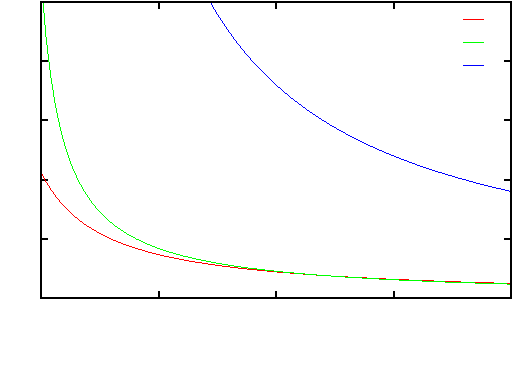
\includegraphics{nucleation_radius}}%
    \gplfronttext
  \end{picture}%
\endgroup
}
%  \label{fig:cnt:critical_number}
%  \subfloat[]{% GNUPLOT: LaTeX picture with Postscript
\begingroup
  \makeatletter
  \providecommand\color[2][]{%
    \GenericError{(gnuplot) \space\space\space\@spaces}{%
      Package color not loaded in conjunction with
      terminal option `colourtext'%
    }{See the gnuplot documentation for explanation.%
    }{Either use 'blacktext' in gnuplot or load the package
      color.sty in LaTeX.}%
    \renewcommand\color[2][]{}%
  }%
  \providecommand\includegraphics[2][]{%
    \GenericError{(gnuplot) \space\space\space\@spaces}{%
      Package graphicx or graphics not loaded%
    }{See the gnuplot documentation for explanation.%
    }{The gnuplot epslatex terminal needs graphicx.sty or graphics.sty.}%
    \renewcommand\includegraphics[2][]{}%
  }%
  \providecommand\rotatebox[2]{#2}%
  \@ifundefined{ifGPcolor}{%
    \newif\ifGPcolor
    \GPcolortrue
  }{}%
  \@ifundefined{ifGPblacktext}{%
    \newif\ifGPblacktext
    \GPblacktexttrue
  }{}%
  % define a \g@addto@macro without @ in the name:
  \let\gplgaddtomacro\g@addto@macro
  % define empty templates for all commands taking text:
  \gdef\gplbacktext{}%
  \gdef\gplfronttext{}%
  \makeatother
  \ifGPblacktext
    % no textcolor at all
    \def\colorrgb#1{}%
    \def\colorgray#1{}%
  \else
    % gray or color?
    \ifGPcolor
      \def\colorrgb#1{\color[rgb]{#1}}%
      \def\colorgray#1{\color[gray]{#1}}%
      \expandafter\def\csname LTw\endcsname{\color{white}}%
      \expandafter\def\csname LTb\endcsname{\color{black}}%
      \expandafter\def\csname LTa\endcsname{\color{black}}%
      \expandafter\def\csname LT0\endcsname{\color[rgb]{1,0,0}}%
      \expandafter\def\csname LT1\endcsname{\color[rgb]{0,1,0}}%
      \expandafter\def\csname LT2\endcsname{\color[rgb]{0,0,1}}%
      \expandafter\def\csname LT3\endcsname{\color[rgb]{1,0,1}}%
      \expandafter\def\csname LT4\endcsname{\color[rgb]{0,1,1}}%
      \expandafter\def\csname LT5\endcsname{\color[rgb]{1,1,0}}%
      \expandafter\def\csname LT6\endcsname{\color[rgb]{0,0,0}}%
      \expandafter\def\csname LT7\endcsname{\color[rgb]{1,0.3,0}}%
      \expandafter\def\csname LT8\endcsname{\color[rgb]{0.5,0.5,0.5}}%
    \else
      % gray
      \def\colorrgb#1{\color{black}}%
      \def\colorgray#1{\color[gray]{#1}}%
      \expandafter\def\csname LTw\endcsname{\color{white}}%
      \expandafter\def\csname LTb\endcsname{\color{black}}%
      \expandafter\def\csname LTa\endcsname{\color{black}}%
      \expandafter\def\csname LT0\endcsname{\color{black}}%
      \expandafter\def\csname LT1\endcsname{\color{black}}%
      \expandafter\def\csname LT2\endcsname{\color{black}}%
      \expandafter\def\csname LT3\endcsname{\color{black}}%
      \expandafter\def\csname LT4\endcsname{\color{black}}%
      \expandafter\def\csname LT5\endcsname{\color{black}}%
      \expandafter\def\csname LT6\endcsname{\color{black}}%
      \expandafter\def\csname LT7\endcsname{\color{black}}%
      \expandafter\def\csname LT8\endcsname{\color{black}}%
    \fi
  \fi
  \setlength{\unitlength}{0.0500bp}%
  \begin{picture}(5040.00,3528.00)%
    \gplgaddtomacro\gplbacktext{%
      \csname LTb\endcsname%
      \put(396,660){\makebox(0,0)[r]{\strut{} 0}}%
      \put(396,1371){\makebox(0,0)[r]{\strut{} 50}}%
      \put(396,2083){\makebox(0,0)[r]{\strut{} 100}}%
      \put(396,2794){\makebox(0,0)[r]{\strut{} 150}}%
      \put(396,3505){\makebox(0,0)[r]{\strut{} 200}}%
      \put(4908,440){\makebox(0,0){\strut{}-2}}%
      \put(3813,440){\makebox(0,0){\strut{}-1.5}}%
      \put(2718,440){\makebox(0,0){\strut{}-1}}%
      \put(1623,440){\makebox(0,0){\strut{}-0.5}}%
      \put(528,440){\makebox(0,0){\strut{} 0}}%
      \put(-374,2082){\rotatebox{90}{\makebox(0,0){\strut{}critical number of molecules}}}%
      \put(2718,110){\makebox(0,0){\strut{}negative pressure (MPa)}}%
    }%
    \gplgaddtomacro\gplfronttext{%
      \csname LTb\endcsname%
      \put(2112,1273){\makebox(0,0)[r]{\strut{}perfluorobutane}}%
      \csname LTb\endcsname%
      \put(2112,1053){\makebox(0,0)[r]{\strut{}perfluoropentane}}%
      \csname LTb\endcsname%
      \put(2112,833){\makebox(0,0)[r]{\strut{}water}}%
    }%
    \gplbacktext
    \put(0,0){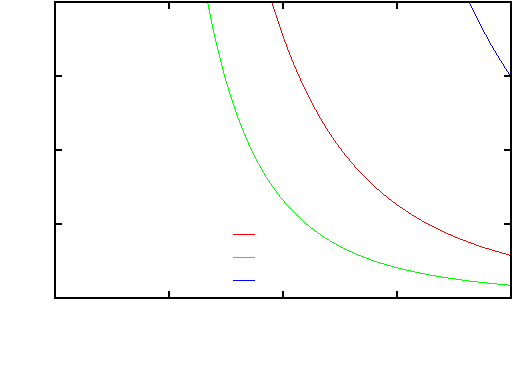
\includegraphics{nucleation_number}}%
    \gplfronttext
  \end{picture}%
\endgroup
}
%  \caption{
%    \Cnt\ predictions for the critical radius and critical number of molecules for a bubble as a function of the pressure.  
%    The vapour is assumed to be an ideal gas, with the vapour pressure obtained by experimental fits to Antoine's equation.
%    The coefficients for Antoine's equation are taken from National Institute of Standards Database\cite{NISTdata}
%    (Note that the perfluorobutane data is used outside of its range of validity, see text).
%  %  The other parameters are taken from the table. \tabref{nuc:parameters}.
%  }
% \label{fig:nucleation_radius}
%\end{figure}
 
%\section{discussion}



%Finally we note that \figref{sppressure} reproduces exactly the result found by Oxtoby\cite{Oxtoby1988}.
%That the vapour spinodal is smaller than the liquid spinodal.
%This was used to explain the difference performance of the classical theory for liquid-bubble cavitation, 
%compared to vapour condensation, (with cavitation doing poorly)




%The final result of the density functional approach, \figref{profile} shows that the thickness of the interface extends over 10 anstrums on each side of the inteface.
%xsThis is extends over most of the bubble wheWhen this compared to the


% \subsection{The density profile}


% For most fluids the interactions are dominated by the strong repulsive forces between the molecules.
% The hard core model is the simplest method of implementing these.
% The pairwise attractive are then treated as a perturbation about the hard core.
% %\begin{align}
% %  F\lrs{\rho(\vr), \rho(\vr^\rpime)} = \fh\lrs{\rho(\vr), \rho(\vr^\rpime)} - \half \phi_{i%j} \rho(\vr_i)\rho(\vr_j)
% %\end{align}
% By writing the joint density $\rho^{(2)} = \rho(\vr)\rho(\vr^\prime)$ we are assuming that there are no correlations in the density distribtution,
% an approximation known as the random phase approximation.

% between most fluids  liquids are well approximated by modelling 
% and so the Free energy can  




% Data for perfluorocarbons in Oh\cite{Oh2010}

%In this chapter we ask the following questions:
%\nlist{
%  \item What is the critical radius of a bubble as a function of pressure.
%  \item At what pressures do we expect the perfluorocarbon oils undergo type 1 nucleation? \label{item:nuc_question1}
 % \item Can the perfluorocarbons be mixed in order to tune the nucleation pressure?\label{item:nuc_question2}
%}
%To answer these questions we need to calculate the  rate of nucleation.
%The bulk of this chapter is dedicated to calculating these rates; first as a function of pressure,
%and second as a function of the perfluorocarbon mixing.
%\todo{get rid of wishful thinking}


%This chapter calculates the pressures required to cavitate perfluorobutane and perfluoropentane
%by using \cnt.
%This is done with classical nucleation theo
% In this chapter we ask At what pressures do we expect the perfluorocarbon oils undergo type 1 nucleation?the following questions:
% \nlist{
%   \item At what pressures do we expect the perfluorocarbon oils undergo type 1 nucleation? \label{item:nuc_question1}
%   \item Can the perfluorocarbons be mixed in order to tune the nucleation pressure?\label{item:nuc_question2}
% }
% To answer these questions we need to calculate the  rate of nucleation.
% The bulk of this chapter is dedicated to calculating these rates; first as a function of pressure,
% and second a
%%%
%
%Theoretical rate calculations areThe nucleation rate has 
%%
%
%he simplest estimate for nucleation rate is provided by  \cnt, which is discussed in \secref{nuc:CNT}.
%This method is essentially an application of the Aarenhius equation.
%The energy barrier to nucleation is found from thermodynamic arguments,
%while the rate is obtained from a kinematic argument.


\subsection{Testing the validity of the capillary approximation}\label{sec:nuc:DFT}
%\begin{quote}
%  An enthusiastic graduate student ... has heard that the density functional approach is {\em the} thing to use but is confused by the plethora of possible approximations.
%Which recipe or recipes do you recommend?  This would be my advice.
%The simple van der Waals approximation is always a good starting point.
%\flushright{Evans}
%\end{quote}
%From \cite{Oxtoby1992}


%\subsubsection{Introduction}

For small bubbles, the assumption of a sharp interface between the bubble and its medium is open to criticism.
Can the width of the interface really be insignificant for a bubble \unit{50}\nano\metre\ wide?
In this section we investigate the issue by taking an alternative approach,
the density functional programme of Oxtoby and Evans\cite{Oxtoby1988}.
%more carefully modelling the interactions at the interface.
%This is done by following the density functional programme of Oxtoby and Evans\cite{Oxtoby1988}.


\Dft\ relaxes the capillary approximation used in \cnt.
The density of the nucleated bubble is not assumed to be uniform,
and the interface is not assumed to be macroscopic and plainer\cite{Oxtoby1992, Oxtoby1988}.
The density functional approach therefore does much better at modelling the interface than \cnt.
Rather than it being a sharp boundary,
there is a finite interval over which the density varies from that of the fluid to that of the vapour.
%However, the density functional approach also models the change in  density across liquid-vapour interface,
%whence removing the flawed capillary approximation from the calculation.
In addition, and as will be shown, the energy barrier to the phase change vanishes at the spinodal.
This is as it should be, but marks a second major improvement on the classical theory\cite{Talanquer1997}.



%and the bubble is modelled for what it is -  a fluctuation in density - 
%rather than a vapour entrapped in  flexible boundary.

%Here we use density functional theory only test the approximations of the classical calculations already carried.
%Density functional theory can be us to calculate the nucleation rate.
%However, it approaches the problem microscopically from a model for the intermolecular potential.
%The calculated rate is, just as in the classical case, exceptionally sensitive to the parameters fed to this model.
%To make quantitative predictions  a semi-empirical approach can be used that fits the parameters to the bulk properties of the fluid\cite{Nyquist1995}.
%Unfortunately, however,  perfluoropentane does not have sufficient data for either the density variations with temperature 
%or the chemical potential variations with temperature.

%This makes qantative predictions unlikeThe vapour pressure 

%\begin{figure}
%  % GNUPLOT: LaTeX picture with Postscript
\begingroup
  \makeatletter
  \providecommand\color[2][]{%
    \GenericError{(gnuplot) \space\space\space\@spaces}{%
      Package color not loaded in conjunction with
      terminal option `colourtext'%
    }{See the gnuplot documentation for explanation.%
    }{Either use 'blacktext' in gnuplot or load the package
      color.sty in LaTeX.}%
    \renewcommand\color[2][]{}%
  }%
  \providecommand\includegraphics[2][]{%
    \GenericError{(gnuplot) \space\space\space\@spaces}{%
      Package graphicx or graphics not loaded%
    }{See the gnuplot documentation for explanation.%
    }{The gnuplot epslatex terminal needs graphicx.sty or graphics.sty.}%
    \renewcommand\includegraphics[2][]{}%
  }%
  \providecommand\rotatebox[2]{#2}%
  \@ifundefined{ifGPcolor}{%
    \newif\ifGPcolor
    \GPcolorfalse
  }{}%
  \@ifundefined{ifGPblacktext}{%
    \newif\ifGPblacktext
    \GPblacktexttrue
  }{}%
  % define a \g@addto@macro without @ in the name:
  \let\gplgaddtomacro\g@addto@macro
  % define empty templates for all commands taking text:
  \gdef\gplbacktext{}%
  \gdef\gplfronttext{}%
  \makeatother
  \ifGPblacktext
    % no textcolor at all
    \def\colorrgb#1{}%
    \def\colorgray#1{}%
  \else
    % gray or color?
    \ifGPcolor
      \def\colorrgb#1{\color[rgb]{#1}}%
      \def\colorgray#1{\color[gray]{#1}}%
      \expandafter\def\csname LTw\endcsname{\color{white}}%
      \expandafter\def\csname LTb\endcsname{\color{black}}%
      \expandafter\def\csname LTa\endcsname{\color{black}}%
      \expandafter\def\csname LT0\endcsname{\color[rgb]{1,0,0}}%
      \expandafter\def\csname LT1\endcsname{\color[rgb]{0,1,0}}%
      \expandafter\def\csname LT2\endcsname{\color[rgb]{0,0,1}}%
      \expandafter\def\csname LT3\endcsname{\color[rgb]{1,0,1}}%
      \expandafter\def\csname LT4\endcsname{\color[rgb]{0,1,1}}%
      \expandafter\def\csname LT5\endcsname{\color[rgb]{1,1,0}}%
      \expandafter\def\csname LT6\endcsname{\color[rgb]{0,0,0}}%
      \expandafter\def\csname LT7\endcsname{\color[rgb]{1,0.3,0}}%
      \expandafter\def\csname LT8\endcsname{\color[rgb]{0.5,0.5,0.5}}%
    \else
      % gray
      \def\colorrgb#1{\color{black}}%
      \def\colorgray#1{\color[gray]{#1}}%
      \expandafter\def\csname LTw\endcsname{\color{white}}%
      \expandafter\def\csname LTb\endcsname{\color{black}}%
      \expandafter\def\csname LTa\endcsname{\color{black}}%
      \expandafter\def\csname LT0\endcsname{\color{black}}%
      \expandafter\def\csname LT1\endcsname{\color{black}}%
      \expandafter\def\csname LT2\endcsname{\color{black}}%
      \expandafter\def\csname LT3\endcsname{\color{black}}%
      \expandafter\def\csname LT4\endcsname{\color{black}}%
      \expandafter\def\csname LT5\endcsname{\color{black}}%
      \expandafter\def\csname LT6\endcsname{\color{black}}%
      \expandafter\def\csname LT7\endcsname{\color{black}}%
      \expandafter\def\csname LT8\endcsname{\color{black}}%
    \fi
  \fi
  \setlength{\unitlength}{0.0500bp}%
  \begin{picture}(5040.00,3528.00)%
    \gplgaddtomacro\gplbacktext{%
      \csname LTb\endcsname%
      \put(1210,704){\makebox(0,0)[r]{\strut{} 0}}%
      \put(1210,1070){\makebox(0,0)[r]{\strut{} 0.5}}%
      \put(1210,1435){\makebox(0,0)[r]{\strut{} 1}}%
      \put(1210,1801){\makebox(0,0)[r]{\strut{} 1.5}}%
      \put(1210,2167){\makebox(0,0)[r]{\strut{} 2}}%
      \put(1210,2533){\makebox(0,0)[r]{\strut{} 2.5}}%
      \put(1210,2898){\makebox(0,0)[r]{\strut{} 3}}%
      \put(1210,3264){\makebox(0,0)[r]{\strut{} 3.5}}%
      \put(1342,484){\makebox(0,0){\strut{} 200}}%
      \put(1791,484){\makebox(0,0){\strut{} 220}}%
      \put(2240,484){\makebox(0,0){\strut{} 240}}%
      \put(2689,484){\makebox(0,0){\strut{} 260}}%
      \put(3138,484){\makebox(0,0){\strut{} 280}}%
      \put(3587,484){\makebox(0,0){\strut{} 300}}%
      \put(4036,484){\makebox(0,0){\strut{} 320}}%
      \put(4485,484){\makebox(0,0){\strut{} 340}}%
      \put(440,1984){\rotatebox{90}{\makebox(0,0){\strut{}vapour pressure, atm}}}%
      \put(3026,154){\makebox(0,0){\strut{}temperature, K}}%
    }%
    \gplgaddtomacro\gplfronttext{%
      \csname LTb\endcsname%
      \put(3058,3091){\makebox(0,0)[r]{\strut{}fit}}%
      \csname LTb\endcsname%
      \put(3058,2871){\makebox(0,0)[r]{\strut{}Barber 1955}}%
      \csname LTb\endcsname%
      \put(3058,2651){\makebox(0,0)[r]{\strut{}Crowder 1967}}%
    }%
    \gplbacktext
    \put(0,0){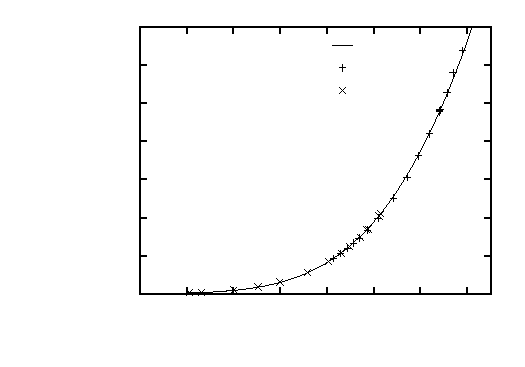
\includegraphics{c2_vapour_pressure_fit}}%
    \gplfronttext
  \end{picture}%
\endgroup

%  \caption{ Fitting the Lennard-Jones model to experimental data for the vapour pressure of perfluoropentane\cite{NISTdata}.
%   However, there is insufficient density data available for perfluoropentane to constrain the data for quantitative measurements.    
%  }
% \label{fig:vapour_pressure}
%\end{figure}
%Data does exist for the vapour pressure as a function of temperature.
%This is used with the single datum  for the density at room temperature to fit the model.
%The result of the fit given in \figref{vapour_pressure}.
%However, enough confidence cannot be placed in the fits to use for quantitative predictions. 
% To use density functional theory toe 

% To calculate the nucleation rate the  Arrhenius form of \eqnref{} is still used.
% The prefactor $J_0$ also remains the same.
% The removal of the capillary approximation changes the expression of the free-energy
% in the exponential.
% It is this quantity that we wish to calculate.

% Rather than starting with thermodynamics, \Dft\ approaches the problem microscopically
 \Dft\ starts by modelling the inter-molecular potentials.
 Good models for the fluid potential exist and 
 among the most widely used are the Lennard-Jones potential
 and the Kihira potential.
 The former describes small spherically symmetric molecules very accurately.
 The latter is a extension on the Lennard-Jones model to describe larger, less symmetric molecules.


In principle, macroscopic predictions can then be drawn by inserting the intermolecular potentials into the usual thermodynamic potentials of statistical mechanics.  
While the full multi-particle potentials are in general insolvable and approximations must be made,
the density functional approach is one derived from a firm theoretical base\cite{Evans1992}.
%the data inputted does not need to be provided.
Unfortunately, when applied to nucleation, the first principles approach  has only ever had qualitative success\cite{Nyquist1995,Talanquer2001},
with the predictions being very sensitive to the modelled molecular scale parameters.
%The nucleation rates still depend exponentially on the predicted energy barrier and small deviations have a profound influence on predictions.
%and the success of the density functional approach to nucleation - without the empirical input - has always only been qualitative

The semi-empirical approach of Nyquist\cite{Nyquist1995} and Talanquer\cite{Talanquer2001}
attempts to temper this sensitivity by fitting the molecular-scale parameters to the experimental data used for the classical theory.
% to making nucleation rate predictions.
% By construction, therefore, the bulk predications of the model are correct. 
By construction, therefore, the bulk thermodynamic predications of the model are correct.
Thermodynamic arguments can then be used to obtain other quantities of interest, such as the nucleation rate. 
We shall use this approach to test the width of interface between the bubble and its medium.
% such as those in equation \eqnref{}.


 %However, by modelling the change in  density across liquid-vapour interface,
 %one of the major flaws of the capillary approximation is removed.
 %In addition with this approach, the energy barrier to the phase change vanishes at the spinodal,
 %a second major correction on the classical theory.


The density functional approach models fluctuations about the bulk properties of the fluid.
It is therefore a mean-field approach that fails, like all mean field theories, near to the critical temperature.
One must be cautious, therefore, only to apply it to nucleation events that occur well away from the critical point.
In this thesis  attention is restricted to nucleation events that are induced by a reduction in pressure 
rather than by boiling.
The critical temperatures for a number of perfluorocarbons are listed in \tabref{nuc:criticalTemps}.
It is interesting to note that for the perfluorocarbons the critical temperatures are considerably higher than their boiling points.
At \unit{37}\degreecelsius, for example, perfluoropentane is in a meta-stable state but is still far from being `on the cusp' of vapourisation.
Type 1 nucleation events are still likely to occur via a reduction in pressure rather than an increase in temperature.
On the other hand, perfluoroethane is above its  critical point at room temperature and we 
consider it to be a little to close to its  critical point to be considered in this thesis.

% The oil chosen for this purpose is perfluoropentane.
% It has the following properties that make it suitable
% \nlist{
% \item
%   it is chemically inert with a low toxicity, \label{nuc:PFP:one} \todo{some references here} 
% \item
%   it has a boiling point of about \unit{28}\degreecelsius. \label{nuc:PFP:two}\todo{some references here to} 
% }
% Property \ref{nuc:PFP:one} is important for any diagnostic contrast agent.
% Property \ref{nuc:PFP:two} suggests that when placed under tension
% \pfp\ should vapourise  more readily than the bulk (assumed to be water).
% This would then give the required selectivity for the contrast agent.
% %It is an oversimplification, however, 
% %to argue that  \pfp's lower boiling point implies that it should form bubbles prior to the bulk.
% %There are multiple mechanisms to bubble nucleation in ultrasound.
% %We argue in \secref{} that the mechanisms for water and \pfp\ droplets are likely to be different,
% %and that the boiling point in the case of water   is not relevant in diagnostic cavitation.

% making a comparison based on the respective physical chemistry incorrect.



%and are then used to derive further
%  so that the model reproduces the 
%correct thermodynamic limit.
%
%While \cnt\ is a useful first calculation,
%it is not adequate to provide quantitative  predictions.
%To overcome these difficulties we employ the semi-empirical density functional approach of Nyquist\cite{Nyquist1995} and Talanquer\cite{Talanquer2001}
%in \secref{nuc:DFT}.
%The {\em semi-empirical} approach uses the same 
%By construction, therefore, the bulk predications of the model are correct. 



% The density functional approach calculates  the free energy 
% directly from the interaction potentials.
% However, as for the classical theory,
% the calculated rates are exponentially sensitive to inaccuracies in the provided model.
% Great care must be taken, therefore, when setting up the models.

% The semi-empiciral approach ...
% Fits so that in the bulk limit...
% DFT then proposes the  details omitted by the classical theory,
% such as finite with of interface.


% Use the approach of Nyquist to calcualate the rate of perlfuorpentane and perfluorbutane.
\subsubsection{Outline of approach}
The approach we will be taking can be summarised as follows:
%In short, the algorithm we shall be using proceeds as follows % The steps that are to be taken are 
 \nlist{
   \item write down an accurate model for the intermolecular potential (\secref{nuc:DFT:write}),
   \item approximate the model so that it can be solved (\secref{nuc:DFT:approx}),
   \item fit the model's parameters so that it reproduces macroscopic thermodynamics (\secref{nuc:DFT:fit}),
   \item predict the shape of the interface between the bubble and its medium and compare it with the capillary approximation (\secref{nuc:DFT:results}).
 }



\subsubsection{The density functional approach}\label{sec:nuc:DFT:write}

The density functional approach is a statistical theory 
that attempts to model the grand potential, $\Omega$,
at a molecular level.
% in \eqnref{nuc:astarR} %is required to evaluate both the rate of nucleation and the critical radius.
%If  spherical symmetry is assumed then 
%the bubble boundary is defined by its radius.
%The critical radius is such that\cite{Oxtoby1992,Oxtoby1988}
%\begin{align}
%  \frac{d \Omega}{d a} =0,\quad\text{at $a = \astar$} \label{eqn:DFT:astarR}
%\end{align}
%where $\Omega$ is the {\em grand potential}.
%
%
%is difficult to evaluate on a microscopic level, however, the grand potential 
The exact solution is intractable due to the mutual interactions between every molecule in the system.
%because it depends upon the free energy, 
%which in turn It is difficult to evaluate
%because the positions of the molecules within the system are not independent,
%but rather depend on the position of every other molecule due to their mutual interactions.
%This is because 
%the intrinsic free energy incorporates the interaction of every molecule with every other molecule in the system.
%Evaluating the intrinsic free energy is then intractable.
%This introduces integrals that are intractable.
%The approach of \dft\ to this problem is standard in statistical physics:

To overcome this problem 
the true probability density function, $p_0(\H; \cx_1,\cp_1)$, that describes 
the positions of the particles and their momenta,
is approximated to a simpler distribution $p(H; \cx_1, \cp_1)$ that may be solved.
Here, $\H$, is the true Hamiltonian of the system 
and $H$ is the approximate Hamiltonian with simpler interaction terms.
We have also employed the  convenient shorthand
\begin{align}
\cx_n \equiv r_n,r_{n+1},\ldots,r_N,  \quad\text{and}\quad
\cp_n \equiv  p_n,p_{n+1},\ldots, p_N.
    \label{eqn:shorthand}
\end{align}
to describe the positions and momenta of  $N-n$ particles.

The {\em relative entropy } or {\em Kullback-Leibler divergance} gives the amount of information lost 
when using the approximate distribution  $p$ rather than the correct distribution $p_0$,
and is defined
\begin{align}
  \KLD{p}{p_0} = \Tr p \log \frac{p}{p_0}, \label{eqn:nuc:KLD}
\end{align}
where $\Tr$ is the classical trace operator. %$\Tr\equiv \sum_{N=0}^\infty \frac{1}{h^{3N}N!} \iint d\cx_1 d\cp_1$ is the classical trace operator.
The relative entropy has the property that 
$\KLD{p}{p_0} \ge 0$, which follows from Gibbs inequality\cite{MacKayBook}.
Only if $p=p_0$ does $\KLD{p}{p_0} = 0$.
Therefore, once the structure of the approximate  distribution $p$ has been chosen,
it can be varied to match to content of $p_0$ as closely as possible by minimising $\KLD{p}{p_0}$.
% In this thesis we consider only pair-wise interactions,
% \begin{align}
% %  \UE(\cx) \approx 
% \Phi(\cx) =  \sum_{j>i} \sum_i^N \phi(\vr_i, \vr_j),
% \end{align}
% where $\phi(\vr_i, \vr_j)$ is the two particle potential between a particle at $r_i$ and $r_j$.
% The structure imposed by higher-order correlations  is ignored by $p$.

Employing this variational procedure to approximate the thermodynamic potentials is ubiquitous in statistical physics\cite{Yedidia2000a}.
The point of departure for the density functional method is the realisation that
\nlist{
\item the {\em density is a functional of the external potential.}
  This follows because the approximation to the  density is related to the single particle probability density function
  \begin{align}
    \rho(\vr) \propto \iint d\cp_1 d\cx_2 p(H, \cx, \cp) \propto  \int e^{-\beta\sum_i^N V_\ext(\vr_i)} d\cx_2
  \end{align}
  where $V_\ext(\vr_i)$ is the external potential at the position $\vr$ of the $i^{th}$ molecule.
  Here were have extended the shorthand  employed in  \eqnref{dshorthand} so that
  \begin{align}
    d\cx_n &\equiv dr_n dr_{n+1}\ldots dr_N, &&\quad\text{and}&
    d\cp_n &\equiv  dp_n dp_{n+1}\ldots dp_N.
    \label{eqn:dshorthand}
  \end{align}
\item {\em the external potential is uniquely determined by the density}.
  This converse result is known as the Hohenberg-Kohn theorem.
%  and an outline of the proof is given in  \appref{DFT}.
  It follows because the external potential is determined by the probability density, $p$, which is in turn determined uniquely by the density.
}
It is thereby permissible to work with the mass density rather than the probability density when considering the thermodynamics of the bubble.
Since the density is the term of interest, the density functional approach is much more direct.
We may therefore define a approximate grand potential, $\Omega_V$, as a functional of the (approximate) density \cite{Evans1992},
\begin{align}
 \Omega_V\lrs{\rho} \equiv \beta^{-1}\KLD{p\lrs{\rho}}{p_0}+   \Omega. 
\end{align}
The approximate  grand potential approaches the true value when
it is minimised with  respect to $\rho$.
Furthermore, since $\Omega$ is the grand potential at thermodynamic equilibrium,
$\Omega_V$ is minimal when $\rho$ describes the  critical density distribution.
The condition of equation \eqnref{nuc:astarR}
can therefore be expressed by the functional derivative\cite{Oxtoby1992}
\begin{align}
  \frac{\delta \Omega_V}{\delta \rho} =0,\quad\text{at $\rho = \rhostar$.} \label{eqn:DFT:astar}
\end{align}


%\subsubsection{The critical bubble}
The grand potential is related to the Helmholtz free energy by a Legendre transformation
\begin{align}
  \Omega_V = F -  \mu \int d\vr \rho(\vr), \label{eqn:OmegaVDefn}
\end{align}
where $\mu$ is the chemical potential.
%The chemical potential is comprised of the two phases of a nucleating bubble:
%the oil and its vapour.
The free energy, $F$, is the sum of  internal energy, $\Phi$, and an  entropic contribution.
The inter-particle interactions are contained within the internal energy.

\subsubsection{Approximate the model}\label{sec:nuc:DFT:approx}
To simplify $F$ it is noted that  the interactions of most fluids are dominated  by volume exclusion effects (van der Waal type interactions).
Longer range interactions are, in general, only of secondary importance\cite{Oxtoby1992}.
If only pair-wise attractions are considered, then the internal energy can then be split into the 
free energy of a {\em hard sphere} reference fluid, $F_\hs$ 
and a small perturbation, $\phi_\attr$, that incorporates the long range attractions.
Then 
\begin{align}
   F\lrs{\rho} = F_\hs\lrs{\rho} +\half   \iint d \vr_i d\vr_j \phi_\attr( \vr_i, \vr_j)\rho(\vr_i, \vr_j),  \label{eqn:F_pert}
\end{align}
where $\phi_\attr(\vr_i, \vr_j)$ is the residual two particle potential between a particle at $\vr_i$ and $\vr_j$,
not incorporated into $F_\hs$.
$\rho(\vr_i, \vr_j) $ is the two particle density function.
(See Evans\cite{Evans1992} for a formal treatment of the above steps).

% \begin{figure}
%  \centering
% %\hspace*{-0.2cm}
%  \label{fig:Kihira_potentials}
%  \subfloat[Kihira 2-particle potentials for various perfluorocarbons]{
%   % GNUPLOT: LaTeX picture with Postscript
\begingroup
  \makeatletter
  \providecommand\color[2][]{%
    \GenericError{(gnuplot) \space\space\space\@spaces}{%
      Package color not loaded in conjunction with
      terminal option `colourtext'%
    }{See the gnuplot documentation for explanation.%
    }{Either use 'blacktext' in gnuplot or load the package
      color.sty in LaTeX.}%
    \renewcommand\color[2][]{}%
  }%
  \providecommand\includegraphics[2][]{%
    \GenericError{(gnuplot) \space\space\space\@spaces}{%
      Package graphicx or graphics not loaded%
    }{See the gnuplot documentation for explanation.%
    }{The gnuplot epslatex terminal needs graphicx.sty or graphics.sty.}%
    \renewcommand\includegraphics[2][]{}%
  }%
  \providecommand\rotatebox[2]{#2}%
  \@ifundefined{ifGPcolor}{%
    \newif\ifGPcolor
    \GPcolortrue
  }{}%
  \@ifundefined{ifGPblacktext}{%
    \newif\ifGPblacktext
    \GPblacktexttrue
  }{}%
  % define a \g@addto@macro without @ in the name:
  \let\gplgaddtomacro\g@addto@macro
  % define empty templates for all commands taking text:
  \gdef\gplbacktext{}%
  \gdef\gplfronttext{}%
  \makeatother
  \ifGPblacktext
    % no textcolor at all
    \def\colorrgb#1{}%
    \def\colorgray#1{}%
  \else
    % gray or color?
    \ifGPcolor
      \def\colorrgb#1{\color[rgb]{#1}}%
      \def\colorgray#1{\color[gray]{#1}}%
      \expandafter\def\csname LTw\endcsname{\color{white}}%
      \expandafter\def\csname LTb\endcsname{\color{black}}%
      \expandafter\def\csname LTa\endcsname{\color{black}}%
      \expandafter\def\csname LT0\endcsname{\color[rgb]{1,0,0}}%
      \expandafter\def\csname LT1\endcsname{\color[rgb]{0,1,0}}%
      \expandafter\def\csname LT2\endcsname{\color[rgb]{0,0,1}}%
      \expandafter\def\csname LT3\endcsname{\color[rgb]{1,0,1}}%
      \expandafter\def\csname LT4\endcsname{\color[rgb]{0,1,1}}%
      \expandafter\def\csname LT5\endcsname{\color[rgb]{1,1,0}}%
      \expandafter\def\csname LT6\endcsname{\color[rgb]{0,0,0}}%
      \expandafter\def\csname LT7\endcsname{\color[rgb]{1,0.3,0}}%
      \expandafter\def\csname LT8\endcsname{\color[rgb]{0.5,0.5,0.5}}%
    \else
      % gray
      \def\colorrgb#1{\color{black}}%
      \def\colorgray#1{\color[gray]{#1}}%
      \expandafter\def\csname LTw\endcsname{\color{white}}%
      \expandafter\def\csname LTb\endcsname{\color{black}}%
      \expandafter\def\csname LTa\endcsname{\color{black}}%
      \expandafter\def\csname LT0\endcsname{\color{black}}%
      \expandafter\def\csname LT1\endcsname{\color{black}}%
      \expandafter\def\csname LT2\endcsname{\color{black}}%
      \expandafter\def\csname LT3\endcsname{\color{black}}%
      \expandafter\def\csname LT4\endcsname{\color{black}}%
      \expandafter\def\csname LT5\endcsname{\color{black}}%
      \expandafter\def\csname LT6\endcsname{\color{black}}%
      \expandafter\def\csname LT7\endcsname{\color{black}}%
      \expandafter\def\csname LT8\endcsname{\color{black}}%
    \fi
  \fi
  \setlength{\unitlength}{0.0500bp}%
  \begin{picture}(3276.00,3276.00)%
    \gplgaddtomacro\gplbacktext{%
      \csname LTb\endcsname%
      \put(341,660){\makebox(0,0)[r]{\strut{}-800}}%
      \put(341,1092){\makebox(0,0)[r]{\strut{}-600}}%
      \put(341,1524){\makebox(0,0)[r]{\strut{}-400}}%
      \put(341,1957){\makebox(0,0)[r]{\strut{}-200}}%
      \put(341,2389){\makebox(0,0)[r]{\strut{} 0}}%
      \put(341,2821){\makebox(0,0)[r]{\strut{} 200}}%
      \put(341,3253){\makebox(0,0)[r]{\strut{} 400}}%
      \put(732,440){\makebox(0,0){\strut{} 6}}%
      \put(1251,440){\makebox(0,0){\strut{} 8}}%
      \put(1770,440){\makebox(0,0){\strut{} 10}}%
      \put(2289,440){\makebox(0,0){\strut{} 12}}%
      \put(2808,440){\makebox(0,0){\strut{} 14}}%
      \put(-165,1956){\rotatebox{90}{\makebox(0,0){\strut{}  $\Phi(r)$ (K)}}}%
      \put(1770,110){\makebox(0,0){\strut{}distance ({\AA })}}%
    }%
    \gplgaddtomacro\gplfronttext{%
      \csname LTb\endcsname%
      \put(2476,3080){\makebox(0,0)[r]{\strut{}$C_4F_{10}-C_4F_{10}$}}%
      \csname LTb\endcsname%
      \put(2476,2860){\makebox(0,0)[r]{\strut{}$C_5F_{12}-C_5F_{12}$}}%
      \csname LTb\endcsname%
      \put(2476,2640){\makebox(0,0)[r]{\strut{}$C_6F_{14}-C_6F_{14}$}}%
    }%
    \gplbacktext
    \put(0,0){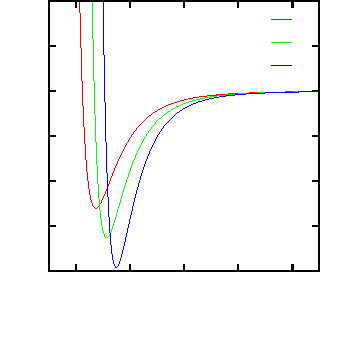
\includegraphics{c2_plot_potentials}}%
    \gplfronttext
  \end{picture}%
\endgroup
}
% \hfill
%  \label{fig:Kihira_WCA}
%  \subfloat[WCA decomposition of the Kihira  potential for perfluoropentane]{
%   % GNUPLOT: LaTeX picture with Postscript
\begingroup
  \makeatletter
  \providecommand\color[2][]{%
    \GenericError{(gnuplot) \space\space\space\@spaces}{%
      Package color not loaded in conjunction with
      terminal option `colourtext'%
    }{See the gnuplot documentation for explanation.%
    }{Either use 'blacktext' in gnuplot or load the package
      color.sty in LaTeX.}%
    \renewcommand\color[2][]{}%
  }%
  \providecommand\includegraphics[2][]{%
    \GenericError{(gnuplot) \space\space\space\@spaces}{%
      Package graphicx or graphics not loaded%
    }{See the gnuplot documentation for explanation.%
    }{The gnuplot epslatex terminal needs graphicx.sty or graphics.sty.}%
    \renewcommand\includegraphics[2][]{}%
  }%
  \providecommand\rotatebox[2]{#2}%
  \@ifundefined{ifGPcolor}{%
    \newif\ifGPcolor
    \GPcolortrue
  }{}%
  \@ifundefined{ifGPblacktext}{%
    \newif\ifGPblacktext
    \GPblacktexttrue
  }{}%
  % define a \g@addto@macro without @ in the name:
  \let\gplgaddtomacro\g@addto@macro
  % define empty templates for all commands taking text:
  \gdef\gplbacktext{}%
  \gdef\gplfronttext{}%
  \makeatother
  \ifGPblacktext
    % no textcolor at all
    \def\colorrgb#1{}%
    \def\colorgray#1{}%
  \else
    % gray or color?
    \ifGPcolor
      \def\colorrgb#1{\color[rgb]{#1}}%
      \def\colorgray#1{\color[gray]{#1}}%
      \expandafter\def\csname LTw\endcsname{\color{white}}%
      \expandafter\def\csname LTb\endcsname{\color{black}}%
      \expandafter\def\csname LTa\endcsname{\color{black}}%
      \expandafter\def\csname LT0\endcsname{\color[rgb]{1,0,0}}%
      \expandafter\def\csname LT1\endcsname{\color[rgb]{0,1,0}}%
      \expandafter\def\csname LT2\endcsname{\color[rgb]{0,0,1}}%
      \expandafter\def\csname LT3\endcsname{\color[rgb]{1,0,1}}%
      \expandafter\def\csname LT4\endcsname{\color[rgb]{0,1,1}}%
      \expandafter\def\csname LT5\endcsname{\color[rgb]{1,1,0}}%
      \expandafter\def\csname LT6\endcsname{\color[rgb]{0,0,0}}%
      \expandafter\def\csname LT7\endcsname{\color[rgb]{1,0.3,0}}%
      \expandafter\def\csname LT8\endcsname{\color[rgb]{0.5,0.5,0.5}}%
    \else
      % gray
      \def\colorrgb#1{\color{black}}%
      \def\colorgray#1{\color[gray]{#1}}%
      \expandafter\def\csname LTw\endcsname{\color{white}}%
      \expandafter\def\csname LTb\endcsname{\color{black}}%
      \expandafter\def\csname LTa\endcsname{\color{black}}%
      \expandafter\def\csname LT0\endcsname{\color{black}}%
      \expandafter\def\csname LT1\endcsname{\color{black}}%
      \expandafter\def\csname LT2\endcsname{\color{black}}%
      \expandafter\def\csname LT3\endcsname{\color{black}}%
      \expandafter\def\csname LT4\endcsname{\color{black}}%
      \expandafter\def\csname LT5\endcsname{\color{black}}%
      \expandafter\def\csname LT6\endcsname{\color{black}}%
      \expandafter\def\csname LT7\endcsname{\color{black}}%
      \expandafter\def\csname LT8\endcsname{\color{black}}%
    \fi
  \fi
  \setlength{\unitlength}{0.0500bp}%
  \begin{picture}(3276.00,3276.00)%
    \gplgaddtomacro\gplbacktext{%
      \csname LTb\endcsname%
      \put(473,660){\makebox(0,0)[r]{\strut{}-800}}%
      \put(473,1092){\makebox(0,0)[r]{\strut{}-600}}%
      \put(473,1524){\makebox(0,0)[r]{\strut{}-400}}%
      \put(473,1957){\makebox(0,0)[r]{\strut{}-200}}%
      \put(473,2389){\makebox(0,0)[r]{\strut{} 0}}%
      \put(473,2821){\makebox(0,0)[r]{\strut{} 200}}%
      \put(473,3253){\makebox(0,0)[r]{\strut{} 400}}%
      \put(605,440){\makebox(0,0){\strut{} 2}}%
      \put(1004,440){\makebox(0,0){\strut{} 4}}%
      \put(1403,440){\makebox(0,0){\strut{} 6}}%
      \put(1802,440){\makebox(0,0){\strut{} 8}}%
      \put(2201,440){\makebox(0,0){\strut{} 10}}%
      \put(2600,440){\makebox(0,0){\strut{} 12}}%
      \put(2999,440){\makebox(0,0){\strut{} 14}}%
      \put(-33,1956){\rotatebox{90}{\makebox(0,0){\strut{}  $\Phi(r)$ (K)}}}%
      \put(1902,110){\makebox(0,0){\strut{}distance ({\AA })}}%
    }%
    \gplgaddtomacro\gplfronttext{%
      \csname LTb\endcsname%
      \put(2608,3080){\makebox(0,0)[r]{\strut{}repulsive}}%
      \csname LTb\endcsname%
      \put(2608,2860){\makebox(0,0)[r]{\strut{}attractive}}%
    }%
    \gplbacktext
    \put(0,0){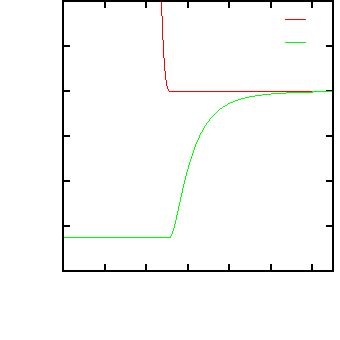
\includegraphics{c2_plot_potentials_WCA}}%
    \gplfronttext
  \end{picture}%
\endgroup
}\\
% \label{fig:Kihira_d}
% \subfloat[Comparison of the WCA repulsive potential with the hard sphere potential]{
%   % GNUPLOT: LaTeX picture with Postscript
\begingroup
  \makeatletter
  \providecommand\color[2][]{%
    \GenericError{(gnuplot) \space\space\space\@spaces}{%
      Package color not loaded in conjunction with
      terminal option `colourtext'%
    }{See the gnuplot documentation for explanation.%
    }{Either use 'blacktext' in gnuplot or load the package
      color.sty in LaTeX.}%
    \renewcommand\color[2][]{}%
  }%
  \providecommand\includegraphics[2][]{%
    \GenericError{(gnuplot) \space\space\space\@spaces}{%
      Package graphicx or graphics not loaded%
    }{See the gnuplot documentation for explanation.%
    }{The gnuplot epslatex terminal needs graphicx.sty or graphics.sty.}%
    \renewcommand\includegraphics[2][]{}%
  }%
  \providecommand\rotatebox[2]{#2}%
  \@ifundefined{ifGPcolor}{%
    \newif\ifGPcolor
    \GPcolortrue
  }{}%
  \@ifundefined{ifGPblacktext}{%
    \newif\ifGPblacktext
    \GPblacktexttrue
  }{}%
  % define a \g@addto@macro without @ in the name:
  \let\gplgaddtomacro\g@addto@macro
  % define empty templates for all commands taking text:
  \gdef\gplbacktext{}%
  \gdef\gplfronttext{}%
  \makeatother
  \ifGPblacktext
    % no textcolor at all
    \def\colorrgb#1{}%
    \def\colorgray#1{}%
  \else
    % gray or color?
    \ifGPcolor
      \def\colorrgb#1{\color[rgb]{#1}}%
      \def\colorgray#1{\color[gray]{#1}}%
      \expandafter\def\csname LTw\endcsname{\color{white}}%
      \expandafter\def\csname LTb\endcsname{\color{black}}%
      \expandafter\def\csname LTa\endcsname{\color{black}}%
      \expandafter\def\csname LT0\endcsname{\color[rgb]{1,0,0}}%
      \expandafter\def\csname LT1\endcsname{\color[rgb]{0,1,0}}%
      \expandafter\def\csname LT2\endcsname{\color[rgb]{0,0,1}}%
      \expandafter\def\csname LT3\endcsname{\color[rgb]{1,0,1}}%
      \expandafter\def\csname LT4\endcsname{\color[rgb]{0,1,1}}%
      \expandafter\def\csname LT5\endcsname{\color[rgb]{1,1,0}}%
      \expandafter\def\csname LT6\endcsname{\color[rgb]{0,0,0}}%
      \expandafter\def\csname LT7\endcsname{\color[rgb]{1,0.3,0}}%
      \expandafter\def\csname LT8\endcsname{\color[rgb]{0.5,0.5,0.5}}%
    \else
      % gray
      \def\colorrgb#1{\color{black}}%
      \def\colorgray#1{\color[gray]{#1}}%
      \expandafter\def\csname LTw\endcsname{\color{white}}%
      \expandafter\def\csname LTb\endcsname{\color{black}}%
      \expandafter\def\csname LTa\endcsname{\color{black}}%
      \expandafter\def\csname LT0\endcsname{\color{black}}%
      \expandafter\def\csname LT1\endcsname{\color{black}}%
      \expandafter\def\csname LT2\endcsname{\color{black}}%
      \expandafter\def\csname LT3\endcsname{\color{black}}%
      \expandafter\def\csname LT4\endcsname{\color{black}}%
      \expandafter\def\csname LT5\endcsname{\color{black}}%
      \expandafter\def\csname LT6\endcsname{\color{black}}%
      \expandafter\def\csname LT7\endcsname{\color{black}}%
      \expandafter\def\csname LT8\endcsname{\color{black}}%
    \fi
  \fi
  \setlength{\unitlength}{0.0500bp}%
  \begin{picture}(5148.00,3276.00)%
    \gplgaddtomacro\gplbacktext{%
      \csname LTb\endcsname%
      \put(396,784){\makebox(0,0)[r]{\strut{}$10^{0}$}}%
      \put(396,1182){\makebox(0,0)[r]{\strut{}$10^{5}$}}%
      \put(396,1580){\makebox(0,0)[r]{\strut{}$10^{10}$}}%
      \put(396,1979){\makebox(0,0)[r]{\strut{}$10^{15}$}}%
      \put(396,2377){\makebox(0,0)[r]{\strut{}$10^{20}$}}%
      \put(396,2775){\makebox(0,0)[r]{\strut{}$10^{25}$}}%
      \put(396,3173){\makebox(0,0)[r]{\strut{}$10^{30}$}}%
      \put(528,484){\makebox(0,0){\strut{} 2}}%
      \put(1051,484){\makebox(0,0){\strut{} 3}}%
      \put(1574,484){\makebox(0,0){\strut{} 4}}%
      \put(2098,484){\makebox(0,0){\strut{} 5}}%
      \put(2621,484){\makebox(0,0){\strut{} 6}}%
      \put(3144,484){\makebox(0,0){\strut{} 7}}%
      \put(3667,484){\makebox(0,0){\strut{} 8}}%
      \put(4190,484){\makebox(0,0){\strut{} 9}}%
      \put(4713,484){\makebox(0,0){\strut{} 10}}%
      \put(-110,1978){\rotatebox{90}{\makebox(0,0){\strut{}  $\Phi(r)$ (K)}}}%
      \put(2673,154){\makebox(0,0){\strut{}distance ({\AA })}}%
    }%
    \gplgaddtomacro\gplfronttext{%
      \csname LTb\endcsname%
      \put(4227,3080){\makebox(0,0)[r]{\strut{}repulsive}}%
      \csname LTb\endcsname%
      \put(4227,2860){\makebox(0,0)[r]{\strut{}core sphere}}%
      \csname LTb\endcsname%
      \put(4227,2640){\makebox(0,0)[r]{\strut{}characteristic}}%
    }%
    \gplbacktext
    \put(0,0){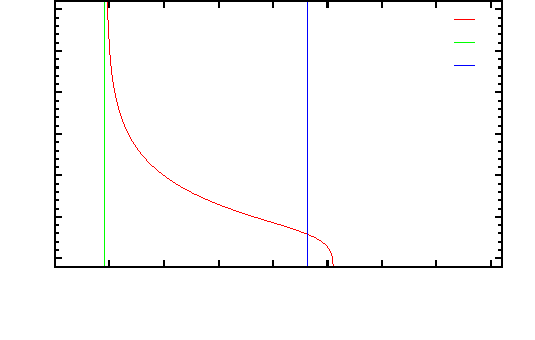
\includegraphics{c2_plot_potentials_WCA_hs}}%
    \gplfronttext
  \end{picture}%
\endgroup
} \hfill
%   \caption{ 
%   }
%  \label{fig:}
% \end{figure}

%All that remains to specify the model is a concrete attractive perturbation.

Next we model the attractive perturbation. 
To do so, we begin with a model for the full two particle interaction 
and then split it into attractive and repulsive parts, according the WCA procedure.
For small symmetric molecules the Lennard-Jones 6-12 potential has good accuracy.
It is given by
\begin{align}
  \phi_\LJ(r) = 4\epsilon\lr{\frac{\sigma^{12}}{r^{12}} - \frac{\sigma^{6}}{r^{6}}}
  \label{eqn:nuc:LJ}
\end{align}
where $r = \abs{\vr=\vr^\prime}$, $\epsilon$ is the characteristic bond energy 
and $\sigma$ the characteristic length.
The Kihira-potential does a better job for larger models such as perfluoropentane 
but greatly complicates the approach.
The Lennard-Jones potential is used  in this thesis.

% The Kihira-potential is an extension to approximate assymmetric molecules.
% It remains a symmetric potential, 
% but it includes a hard sphere of radius $r$ of excluded volume.
% \begin{align}
%   \phi_\K(r) = 4\epsilon\lr{\frac{\lr{\sigma-2a}^{12}}{\lr{r-2a}^{12}} - \frac{\lr{\sigma-2a}^{6}}{\lr{r-2a}^{6}}}
% \end{align}
% Oh\cite{Oh2010} recently fitted the Kihira-potential to the measured  second viral coefficient and viscosity 
% of the perlfuoroalkane series.
% The calculated potentials are plotted in \figref{Kihira_potentials}

The potentials are then separated into attractive and repulsive parts, $\phi_\attr$ and $\phi_\rep$, respectively,
\begin{align}
  \phi_\rep^\WCA(r) = \left\{
    \begin{array}{ll}
      \phi(r) +  \epsilon & \text{if $r<r_\min$}\\
      0 & \text{otherwise}
    \end{array} \right. 
\end{align}
and 
\begin{align}
  \phi_\attr^\WCA(r) = \left\{ 
    \begin{array}{ll}
      - \epsilon & \text{if $r<r_\min$}\\
      \phi(r) & \text{otherwise}
    \end{array} \right.
\end{align}
where $r_\min$ is the radius at which the potential is minimal.

It is useful at this stage to define the integrated strength of the attractive potential, 
\begin{align}
  \alpha =  - \iint d \vr_i d\vr_j \phi_\attr( \vr_i, \vr_j).
  \label{eqn:nuc:alpha}
\end{align}

Finally to re-establish contact with the hard sphere approximation 
the repulsive part of the decomposition is replaced by an infinite repulsion at a distance $d$,
That is 
\begin{align}
  \phi_\hs(r) = \left\{
    \begin{array}{ll}
      \infty & \text{if $r<d$}\\
      0 & \text{otherwise}
    \end{array} \right. .
\end{align}

%This WCA decomposition is plotted for \pfp\ in \figref{Kihira_WCA}.
%\subsubsection{Approximations}
Equation \eqnref{F_pert} is still exact for two particle potential theories.
In order to solve it we first  assume that the  hard sphere potential is a function only of the local density,
\begin{align}
  F_\hs \lrs{\rho} \approx \int d\vr f_\hs(\rho(\vr)). \label{eqn:LDA}
\end{align}
$f_\hs(\rho(\vr))$ is the potential (per unit volume) of a uniform  hard-sphere fluid\cite{Evans1992}.
It is obtained from the accurate  Carnahan-Stirling equation of state,
\begin{align}
    \fh(\rho(\vr)) =  f_\ideal + \rho \kB T\frac{4\eta - 3\eta^2}{\lr{1-\eta}^2}
  \label{eqn:nuc:CS}
\end{align}
where $\eta =  \frac{\pi \rho d^3}{6}$ is the packing function and $f_\ideal =  \rho\kB T\lr{\ln \lr{\rho \lambda^3} -1}$ is the free energy (per volume) of an ideal gas.
$\lambda$ is the de Broglie wavelength.
%
%\begin{align}
%  f_\hs(\rho) = p_\hs + \mu \rho.
%\end{align}
%$f_\hs(\rho(\vr))$ can be obtained from the accurate Carnahan-Stirling equation of state.
%It is  a known (but non-linear) function of the number density.
The approximation \eqnref{LDA} is known as the {\em local-density approximation}.

The perturbation may be approximated by assuming that the two particle densities are uncorrelated, 
\begin{align}
\rho(\vr_i, \vr_j) \approx \rho(\vr_i)\rho(\vr_j).\label{eqn:RPA}
\end{align}
This is known as the {\em random phase approximation}.
%The approximation has been found to be accurate in the absence of rapid \todo{get this sentence right} \cite.
If the medium is sufficiently large then this approximation should hold\cite{Evans1992}.
The random phase approximation may well need to be refined for very small oil droplet in water,  
where the oil-water interface cannot be ignored.

Equation \eqnref{OmegaVDefn} can therefore be written as an explicit function of $\rho$,
\begin{align}
   \Omega_V = \int d\vr f_\hs(\rho(\vr))  +   \iint d \vr_i d\vr_j \phi_\attr( \vr_i, \vr_j) \rho(\vr_i)\rho(\vr_j) -  \mu \int d\vr \rho(\vr),  \label{eqn:OmegaV}
\end{align}
where equations \eqnref{F_pert}, \eqnref{LDA} and \eqnref{RPA} have been used.
Minimising \eqnref{OmegaV} with respect to $\rho(\vr)$ gives
\begin{align}
  \frac{\delta  f_\hs(\rho(\vr)) }{\delta \rho(\vr)} \equiv \mu_\hs\lrs{\rho(\vr)} = \mu - \int d\vr^\prime \phi_\attr( \vr, \vr^\prime) \rho(\vr^\prime). \label{eqn:ChemPots}
\end{align}
$\mu_\hs\lrs{\rho(\vr)}$ is the chemical potential of the hard sphere fluid\footnote{
The chemical potential of a hard sphere fluid is given by 
\begin{align}
 \mu_\hs = \frac{d \fh}{d \rho} =  \kB T\frac{8\eta - 9 \eta^2 + 3\eta^3}{\lr{1-\eta}^3} + \kB \ln \lr{\rho \lambda^3}
\end{align}
}.

All the terms on in \eqnref{ChemPots} can be obtained for a given function density profile.
$\mu_\hs$ on the left and the second term on the right hand side have explicit representations, while
the chemical potential $\mu$ `mean field' is obtained by analysing the bulk properties of the fluid.
Equation \eqnref{ChemPots} can therefore be solved by iteration.
An initial guess as the density profile is given to the right hand side.
The chemical potential $\mu_\hs$ is then inverted (numerically) to give an improved estimate of $\rho$.
%This procedure is carried out for the perfluorocarbons in \secref{}.

The density obtained by solving \eqnref{ChemPots} is the density that minimises $\Omega_V$,
and it therefore gives the best approximation the true equilibrium grand potential.
The bubble is only in thermodynamic equilibrium when it is at its critical radius.
Therefore the density $\rho$ obtained from \eqnref{ChemPots} is the density profile of the critical bubble.
%With this we may obtain an improved estimate of the surface tension and estimate a more reliable nucleation rate.

\subsubsection{Fit the model parameters}\label{sec:nuc:DFT:fit}

To use equation \eqnref{ChemPots} 
we need to define the free parameters in our model.
There are four parameters in total, of which three are independent,
\nlist{
\item $\epsilon$ - the energy scale in the Lennard-Jones 6-12 potential (equation \eqnref{nuc:LJ}),
\item $\sigma$ - the length scale in the Lennard-Jones 6-12 potential (equation \eqnref{nuc:LJ}),
\item $\alpha$ - the attractive strength of the Lennard-Jones 6-12 potential (equation \eqnref{nuc:alpha}),
\item $d$ - The length scale in the hard-sphere model (equation \eqnref{nuc:CS}).
}

Two of the parameters can be set by considering the bulk fluid.
If the density is uniform then equation \eqnref{OmegaV} becomes
\begin{align}
   \Omega_V/V =  f_\hs(\rho)  -  \tfrac{1}{2}\alpha \rho^2 -  \mu \rho= p_\hs + \mu_\hs \rho  -  \tfrac{1}{2} \alpha \rho^2 -  \mu \rho. \label{eqn:nuc:OmegaVBulk}
\end{align}
where $V$ is the volume of the system%. %and 
%\begin{align}
%  \alpha =  - \iint d \vr_i d\vr_j \phi_\attr( \vr_i, \vr_j)
%\end{align}
%is the total attractive contribution from the perturbation.
\footnote{The hard sphere pressure is given by
\begin{align}
 p_\hs = \kB T \rho \frac{1+\eta +\eta^2-\eta^3}{1-\eta^3}. \label{eqn:nuc:HSpressure}
\end{align}
}.

Equation \Eqnref{nuc:OmegaVBulk}  can be minimised with the help of the Maxwell relation
\begin{align}
  \frac{\d p_\hs}{\d \rho} = \rho \frac{\d \mu_\hs}{\d \rho} 
\end{align}
to obtain
\begin{align}
  \mu = \mu_\hs - \alpha \rho. \label{eqn:nuc:muBulk}
\end{align}
Substituting \eqnref{nuc:muBulk} into \eqnref{nuc:OmegaVBulk} gives
\begin{align}
   \Omega_V/V = -p_\hs(\rho) + \half \alpha \rho^2 = -p.
   \label{eqn:nuc:OmegaVBulkP}
\end{align}
Equation \eqnref{nuc:OmegaVBulkP} depends only on $d$ and $\alpha$.

Below the critical temperature there will be 
two phases in  bulk coexistence.
The number densities of these two phases are $\rho_v$ and $\rho_L$,
where the ``$v$'' denotes the vapour and the ``$L$'' denotes the liquid.
%as in \secref{nuc:CNT}.
At equilibrium the chemical potential and the pressures for both phases are equal
\sub{
\label{eqn:BulkCoex}
\begin{align}
  \mu_v = \mu_\hs(\rho_v) - \alpha \rho_v &= \mu_\hs(\rho_L) - \alpha \rho_L = \mu_L,\\
  p_v = p_\hs(\rho_v) - \half \alpha \rho_v^2 &= p_\hs(\rho_L) - \half \alpha \rho_L^2 = p_L.
\end{align}
}
The solutions of equations \eqnref{BulkCoex} define the coexistence curve for the fluid,
and they may be used to obtain the two parameters $d$ and $\alpha$.

The final parameter, $\sigma$ (or equivalently $\epsilon$) is obtained from the measured surface tension of the fluid.
The value of $\Omega$ is obtained by iterating \eqnref{ChemPots}.  
The surface tension is then calculated by noting that
\begin{align}
  \Omega_V = \Omega_{V_l} + \Omega_{V_g} + \gamma A,
\end{align}
where $\Omega_{V_l}$ and $\Omega_{V_g}$ are the potentials of the bulk liquid and gas evaluated at the Gibbs surface,
$\gamma$ is the surface tension and $A$ is the area of the surface.
The value of $\sigma$ is chosen so that the calculated value of $\gamma$ matches its experimental value.


The code to solve these equations was written by the author of this thesis and is freely available on github\cite{NucleationCode}.

\subsection{Results of the density functional approach}\label{sec:nuc:DFT:results}


\begin{figure}
  \hspace*{-8mm}
  \subfloat[Coexistence for water]{% GNUPLOT: LaTeX picture with Postscript
\begingroup
  \makeatletter
  \providecommand\color[2][]{%
    \GenericError{(gnuplot) \space\space\space\@spaces}{%
      Package color not loaded in conjunction with
      terminal option `colourtext'%
    }{See the gnuplot documentation for explanation.%
    }{Either use 'blacktext' in gnuplot or load the package
      color.sty in LaTeX.}%
    \renewcommand\color[2][]{}%
  }%
  \providecommand\includegraphics[2][]{%
    \GenericError{(gnuplot) \space\space\space\@spaces}{%
      Package graphicx or graphics not loaded%
    }{See the gnuplot documentation for explanation.%
    }{The gnuplot epslatex terminal needs graphicx.sty or graphics.sty.}%
    \renewcommand\includegraphics[2][]{}%
  }%
  \providecommand\rotatebox[2]{#2}%
  \@ifundefined{ifGPcolor}{%
    \newif\ifGPcolor
    \GPcolorfalse
  }{}%
  \@ifundefined{ifGPblacktext}{%
    \newif\ifGPblacktext
    \GPblacktexttrue
  }{}%
  % define a \g@addto@macro without @ in the name:
  \let\gplgaddtomacro\g@addto@macro
  % define empty templates for all commands taking text:
  \gdef\gplbacktext{}%
  \gdef\gplfronttext{}%
  \makeatother
  \ifGPblacktext
    % no textcolor at all
    \def\colorrgb#1{}%
    \def\colorgray#1{}%
  \else
    % gray or color?
    \ifGPcolor
      \def\colorrgb#1{\color[rgb]{#1}}%
      \def\colorgray#1{\color[gray]{#1}}%
      \expandafter\def\csname LTw\endcsname{\color{white}}%
      \expandafter\def\csname LTb\endcsname{\color{black}}%
      \expandafter\def\csname LTa\endcsname{\color{black}}%
      \expandafter\def\csname LT0\endcsname{\color[rgb]{1,0,0}}%
      \expandafter\def\csname LT1\endcsname{\color[rgb]{0,1,0}}%
      \expandafter\def\csname LT2\endcsname{\color[rgb]{0,0,1}}%
      \expandafter\def\csname LT3\endcsname{\color[rgb]{1,0,1}}%
      \expandafter\def\csname LT4\endcsname{\color[rgb]{0,1,1}}%
      \expandafter\def\csname LT5\endcsname{\color[rgb]{1,1,0}}%
      \expandafter\def\csname LT6\endcsname{\color[rgb]{0,0,0}}%
      \expandafter\def\csname LT7\endcsname{\color[rgb]{1,0.3,0}}%
      \expandafter\def\csname LT8\endcsname{\color[rgb]{0.5,0.5,0.5}}%
    \else
      % gray
      \def\colorrgb#1{\color{black}}%
      \def\colorgray#1{\color[gray]{#1}}%
      \expandafter\def\csname LTw\endcsname{\color{white}}%
      \expandafter\def\csname LTb\endcsname{\color{black}}%
      \expandafter\def\csname LTa\endcsname{\color{black}}%
      \expandafter\def\csname LT0\endcsname{\color{black}}%
      \expandafter\def\csname LT1\endcsname{\color{black}}%
      \expandafter\def\csname LT2\endcsname{\color{black}}%
      \expandafter\def\csname LT3\endcsname{\color{black}}%
      \expandafter\def\csname LT4\endcsname{\color{black}}%
      \expandafter\def\csname LT5\endcsname{\color{black}}%
      \expandafter\def\csname LT6\endcsname{\color{black}}%
      \expandafter\def\csname LT7\endcsname{\color{black}}%
      \expandafter\def\csname LT8\endcsname{\color{black}}%
    \fi
  \fi
  \setlength{\unitlength}{0.0500bp}%
  \begin{picture}(7200.00,5040.00)%
    \gplgaddtomacro\gplbacktext{%
      \csname LTb\endcsname%
      \put(946,704){\makebox(0,0)[r]{\strut{} 250}}%
      \put(946,1213){\makebox(0,0)[r]{\strut{} 300}}%
      \put(946,1722){\makebox(0,0)[r]{\strut{} 350}}%
      \put(946,2231){\makebox(0,0)[r]{\strut{} 400}}%
      \put(946,2740){\makebox(0,0)[r]{\strut{} 450}}%
      \put(946,3248){\makebox(0,0)[r]{\strut{} 500}}%
      \put(946,3757){\makebox(0,0)[r]{\strut{} 550}}%
      \put(946,4266){\makebox(0,0)[r]{\strut{} 600}}%
      \put(946,4775){\makebox(0,0)[r]{\strut{} 650}}%
      \put(1078,484){\makebox(0,0){\strut{} 0}}%
      \put(1651,484){\makebox(0,0){\strut{} 100}}%
      \put(2223,484){\makebox(0,0){\strut{} 200}}%
      \put(2796,484){\makebox(0,0){\strut{} 300}}%
      \put(3368,484){\makebox(0,0){\strut{} 400}}%
      \put(3941,484){\makebox(0,0){\strut{} 500}}%
      \put(4513,484){\makebox(0,0){\strut{} 600}}%
      \put(5086,484){\makebox(0,0){\strut{} 700}}%
      \put(5658,484){\makebox(0,0){\strut{} 800}}%
      \put(6231,484){\makebox(0,0){\strut{} 900}}%
      \put(6803,484){\makebox(0,0){\strut{} 1000}}%
      \put(176,2739){\rotatebox{-270}{\makebox(0,0){\strut{}temperature ($K$)}}}%
      \put(3940,154){\makebox(0,0){\strut{}density ($kg/m^3$)}}%
    }%
    \gplgaddtomacro\gplfronttext{%
      \csname LTb\endcsname%
      \put(5816,4602){\makebox(0,0)[r]{\strut{}coexistence}}%
      \csname LTb\endcsname%
      \put(5816,4382){\makebox(0,0)[r]{\strut{}measured}}%
      \csname LTb\endcsname%
      \put(5816,4162){\makebox(0,0)[r]{\strut{}spinodal}}%
    }%
    \gplbacktext
    \put(0,0){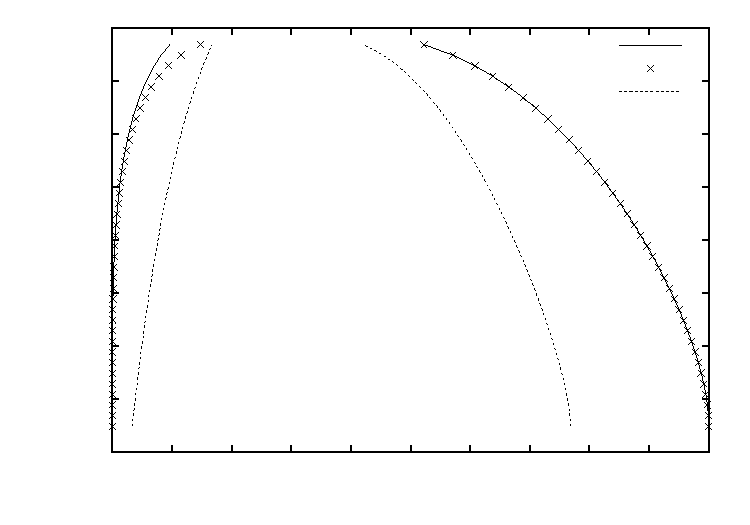
\includegraphics{chNucCoexWater}}%
    \gplfronttext
  \end{picture}%
\endgroup
}\\
  \hspace*{-8mm}
  \subfloat[Coexistence for \pfp]{% GNUPLOT: LaTeX picture with Postscript
\begingroup
  \makeatletter
  \providecommand\color[2][]{%
    \GenericError{(gnuplot) \space\space\space\@spaces}{%
      Package color not loaded in conjunction with
      terminal option `colourtext'%
    }{See the gnuplot documentation for explanation.%
    }{Either use 'blacktext' in gnuplot or load the package
      color.sty in LaTeX.}%
    \renewcommand\color[2][]{}%
  }%
  \providecommand\includegraphics[2][]{%
    \GenericError{(gnuplot) \space\space\space\@spaces}{%
      Package graphicx or graphics not loaded%
    }{See the gnuplot documentation for explanation.%
    }{The gnuplot epslatex terminal needs graphicx.sty or graphics.sty.}%
    \renewcommand\includegraphics[2][]{}%
  }%
  \providecommand\rotatebox[2]{#2}%
  \@ifundefined{ifGPcolor}{%
    \newif\ifGPcolor
    \GPcolorfalse
  }{}%
  \@ifundefined{ifGPblacktext}{%
    \newif\ifGPblacktext
    \GPblacktexttrue
  }{}%
  % define a \g@addto@macro without @ in the name:
  \let\gplgaddtomacro\g@addto@macro
  % define empty templates for all commands taking text:
  \gdef\gplbacktext{}%
  \gdef\gplfronttext{}%
  \makeatother
  \ifGPblacktext
    % no textcolor at all
    \def\colorrgb#1{}%
    \def\colorgray#1{}%
  \else
    % gray or color?
    \ifGPcolor
      \def\colorrgb#1{\color[rgb]{#1}}%
      \def\colorgray#1{\color[gray]{#1}}%
      \expandafter\def\csname LTw\endcsname{\color{white}}%
      \expandafter\def\csname LTb\endcsname{\color{black}}%
      \expandafter\def\csname LTa\endcsname{\color{black}}%
      \expandafter\def\csname LT0\endcsname{\color[rgb]{1,0,0}}%
      \expandafter\def\csname LT1\endcsname{\color[rgb]{0,1,0}}%
      \expandafter\def\csname LT2\endcsname{\color[rgb]{0,0,1}}%
      \expandafter\def\csname LT3\endcsname{\color[rgb]{1,0,1}}%
      \expandafter\def\csname LT4\endcsname{\color[rgb]{0,1,1}}%
      \expandafter\def\csname LT5\endcsname{\color[rgb]{1,1,0}}%
      \expandafter\def\csname LT6\endcsname{\color[rgb]{0,0,0}}%
      \expandafter\def\csname LT7\endcsname{\color[rgb]{1,0.3,0}}%
      \expandafter\def\csname LT8\endcsname{\color[rgb]{0.5,0.5,0.5}}%
    \else
      % gray
      \def\colorrgb#1{\color{black}}%
      \def\colorgray#1{\color[gray]{#1}}%
      \expandafter\def\csname LTw\endcsname{\color{white}}%
      \expandafter\def\csname LTb\endcsname{\color{black}}%
      \expandafter\def\csname LTa\endcsname{\color{black}}%
      \expandafter\def\csname LT0\endcsname{\color{black}}%
      \expandafter\def\csname LT1\endcsname{\color{black}}%
      \expandafter\def\csname LT2\endcsname{\color{black}}%
      \expandafter\def\csname LT3\endcsname{\color{black}}%
      \expandafter\def\csname LT4\endcsname{\color{black}}%
      \expandafter\def\csname LT5\endcsname{\color{black}}%
      \expandafter\def\csname LT6\endcsname{\color{black}}%
      \expandafter\def\csname LT7\endcsname{\color{black}}%
      \expandafter\def\csname LT8\endcsname{\color{black}}%
    \fi
  \fi
  \setlength{\unitlength}{0.0500bp}%
  \begin{picture}(7200.00,5040.00)%
    \gplgaddtomacro\gplbacktext{%
      \csname LTb\endcsname%
      \put(946,704){\makebox(0,0)[r]{\strut{} 200}}%
      \put(946,1518){\makebox(0,0)[r]{\strut{} 250}}%
      \put(946,2332){\makebox(0,0)[r]{\strut{} 300}}%
      \put(946,3147){\makebox(0,0)[r]{\strut{} 350}}%
      \put(946,3961){\makebox(0,0)[r]{\strut{} 400}}%
      \put(946,4775){\makebox(0,0)[r]{\strut{} 450}}%
      \put(1078,484){\makebox(0,0){\strut{} 0}}%
      \put(1651,484){\makebox(0,0){\strut{} 200}}%
      \put(2223,484){\makebox(0,0){\strut{} 400}}%
      \put(2796,484){\makebox(0,0){\strut{} 600}}%
      \put(3368,484){\makebox(0,0){\strut{} 800}}%
      \put(3941,484){\makebox(0,0){\strut{} 1000}}%
      \put(4513,484){\makebox(0,0){\strut{} 1200}}%
      \put(5086,484){\makebox(0,0){\strut{} 1400}}%
      \put(5658,484){\makebox(0,0){\strut{} 1600}}%
      \put(6231,484){\makebox(0,0){\strut{} 1800}}%
      \put(6803,484){\makebox(0,0){\strut{} 2000}}%
      \put(176,2739){\rotatebox{-270}{\makebox(0,0){\strut{}temperature ($K$)}}}%
      \put(3940,154){\makebox(0,0){\strut{}density ($kg/m^3$)}}%
    }%
    \gplgaddtomacro\gplfronttext{%
      \csname LTb\endcsname%
      \put(5816,4602){\makebox(0,0)[r]{\strut{}coexistence}}%
      \csname LTb\endcsname%
      \put(5816,4382){\makebox(0,0)[r]{\strut{}measured}}%
      \csname LTb\endcsname%
      \put(5816,4162){\makebox(0,0)[r]{\strut{}spinodal}}%
    }%
    \gplbacktext
    \put(0,0){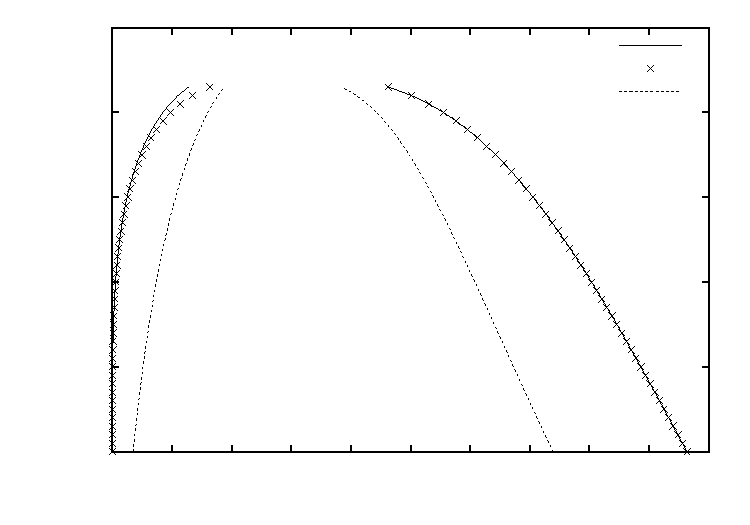
\includegraphics{chNucCoexPfp}}%
    \gplfronttext
  \end{picture}%
\endgroup
}
  \caption{Coexistence and spinodal curve for water and \pfp.
    The plot was used to obtain the temperature dependence of the parameters $d$ and $\epsilon$ 
    in the hard-sphere model with Lennard-Jones interactions.
  }
 \label{fig:nuc:coex}
\end{figure}

\begin{figure}
  \hspace*{-22mm}
  \subfloat[The parameter $d$ for water]{% GNUPLOT: LaTeX picture with Postscript
\begingroup
  \makeatletter
  \providecommand\color[2][]{%
    \GenericError{(gnuplot) \space\space\space\@spaces}{%
      Package color not loaded in conjunction with
      terminal option `colourtext'%
    }{See the gnuplot documentation for explanation.%
    }{Either use 'blacktext' in gnuplot or load the package
      color.sty in LaTeX.}%
    \renewcommand\color[2][]{}%
  }%
  \providecommand\includegraphics[2][]{%
    \GenericError{(gnuplot) \space\space\space\@spaces}{%
      Package graphicx or graphics not loaded%
    }{See the gnuplot documentation for explanation.%
    }{The gnuplot epslatex terminal needs graphicx.sty or graphics.sty.}%
    \renewcommand\includegraphics[2][]{}%
  }%
  \providecommand\rotatebox[2]{#2}%
  \@ifundefined{ifGPcolor}{%
    \newif\ifGPcolor
    \GPcolorfalse
  }{}%
  \@ifundefined{ifGPblacktext}{%
    \newif\ifGPblacktext
    \GPblacktexttrue
  }{}%
  % define a \g@addto@macro without @ in the name:
  \let\gplgaddtomacro\g@addto@macro
  % define empty templates for all commands taking text:
  \gdef\gplbacktext{}%
  \gdef\gplfronttext{}%
  \makeatother
  \ifGPblacktext
    % no textcolor at all
    \def\colorrgb#1{}%
    \def\colorgray#1{}%
  \else
    % gray or color?
    \ifGPcolor
      \def\colorrgb#1{\color[rgb]{#1}}%
      \def\colorgray#1{\color[gray]{#1}}%
      \expandafter\def\csname LTw\endcsname{\color{white}}%
      \expandafter\def\csname LTb\endcsname{\color{black}}%
      \expandafter\def\csname LTa\endcsname{\color{black}}%
      \expandafter\def\csname LT0\endcsname{\color[rgb]{1,0,0}}%
      \expandafter\def\csname LT1\endcsname{\color[rgb]{0,1,0}}%
      \expandafter\def\csname LT2\endcsname{\color[rgb]{0,0,1}}%
      \expandafter\def\csname LT3\endcsname{\color[rgb]{1,0,1}}%
      \expandafter\def\csname LT4\endcsname{\color[rgb]{0,1,1}}%
      \expandafter\def\csname LT5\endcsname{\color[rgb]{1,1,0}}%
      \expandafter\def\csname LT6\endcsname{\color[rgb]{0,0,0}}%
      \expandafter\def\csname LT7\endcsname{\color[rgb]{1,0.3,0}}%
      \expandafter\def\csname LT8\endcsname{\color[rgb]{0.5,0.5,0.5}}%
    \else
      % gray
      \def\colorrgb#1{\color{black}}%
      \def\colorgray#1{\color[gray]{#1}}%
      \expandafter\def\csname LTw\endcsname{\color{white}}%
      \expandafter\def\csname LTb\endcsname{\color{black}}%
      \expandafter\def\csname LTa\endcsname{\color{black}}%
      \expandafter\def\csname LT0\endcsname{\color{black}}%
      \expandafter\def\csname LT1\endcsname{\color{black}}%
      \expandafter\def\csname LT2\endcsname{\color{black}}%
      \expandafter\def\csname LT3\endcsname{\color{black}}%
      \expandafter\def\csname LT4\endcsname{\color{black}}%
      \expandafter\def\csname LT5\endcsname{\color{black}}%
      \expandafter\def\csname LT6\endcsname{\color{black}}%
      \expandafter\def\csname LT7\endcsname{\color{black}}%
      \expandafter\def\csname LT8\endcsname{\color{black}}%
    \fi
  \fi
  \setlength{\unitlength}{0.0500bp}%
  \begin{picture}(4320.00,3024.00)%
    \gplgaddtomacro\gplbacktext{%
      \csname LTb\endcsname%
      \put(990,704){\makebox(0,0)[r]{\strut{} 0.294}}%
      \put(990,910){\makebox(0,0)[r]{\strut{} 0.296}}%
      \put(990,1115){\makebox(0,0)[r]{\strut{} 0.298}}%
      \put(990,1321){\makebox(0,0)[r]{\strut{} 0.3}}%
      \put(990,1526){\makebox(0,0)[r]{\strut{} 0.302}}%
      \put(990,1732){\makebox(0,0)[r]{\strut{} 0.304}}%
      \put(990,1937){\makebox(0,0)[r]{\strut{} 0.306}}%
      \put(990,2143){\makebox(0,0)[r]{\strut{} 0.308}}%
      \put(990,2348){\makebox(0,0)[r]{\strut{} 0.31}}%
      \put(990,2554){\makebox(0,0)[r]{\strut{} 0.312}}%
      \put(990,2759){\makebox(0,0)[r]{\strut{} 0.314}}%
      \put(1122,484){\makebox(0,0){\strut{} 250}}%
      \put(1522,484){\makebox(0,0){\strut{} 300}}%
      \put(1921,484){\makebox(0,0){\strut{} 350}}%
      \put(2321,484){\makebox(0,0){\strut{} 400}}%
      \put(2721,484){\makebox(0,0){\strut{} 450}}%
      \put(3120,484){\makebox(0,0){\strut{} 500}}%
      \put(3520,484){\makebox(0,0){\strut{} 550}}%
      \put(3919,484){\makebox(0,0){\strut{} 600}}%
      \put(4319,484){\makebox(0,0){\strut{} 650}}%
      \put(352,1731){\rotatebox{-270}{\makebox(0,0){\strut{}$d$ ($nm$)}}}%
      \put(2720,154){\makebox(0,0){\strut{}temperature ($K$)}}%
    }%
    \gplgaddtomacro\gplfronttext{%
    }%
    \gplbacktext
    \put(0,0){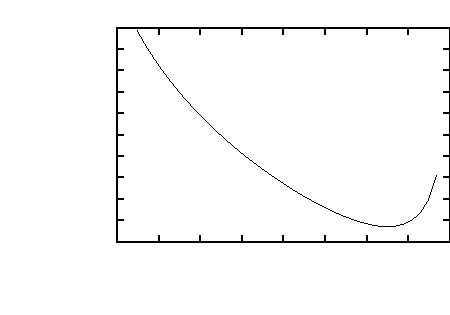
\includegraphics{chNucParamsDWater}}%
    \gplfronttext
  \end{picture}%
\endgroup
}
  \subfloat[The parameter $\mu$ for  water]{% GNUPLOT: LaTeX picture with Postscript
\begingroup
  \makeatletter
  \providecommand\color[2][]{%
    \GenericError{(gnuplot) \space\space\space\@spaces}{%
      Package color not loaded in conjunction with
      terminal option `colourtext'%
    }{See the gnuplot documentation for explanation.%
    }{Either use 'blacktext' in gnuplot or load the package
      color.sty in LaTeX.}%
    \renewcommand\color[2][]{}%
  }%
  \providecommand\includegraphics[2][]{%
    \GenericError{(gnuplot) \space\space\space\@spaces}{%
      Package graphicx or graphics not loaded%
    }{See the gnuplot documentation for explanation.%
    }{The gnuplot epslatex terminal needs graphicx.sty or graphics.sty.}%
    \renewcommand\includegraphics[2][]{}%
  }%
  \providecommand\rotatebox[2]{#2}%
  \@ifundefined{ifGPcolor}{%
    \newif\ifGPcolor
    \GPcolorfalse
  }{}%
  \@ifundefined{ifGPblacktext}{%
    \newif\ifGPblacktext
    \GPblacktexttrue
  }{}%
  % define a \g@addto@macro without @ in the name:
  \let\gplgaddtomacro\g@addto@macro
  % define empty templates for all commands taking text:
  \gdef\gplbacktext{}%
  \gdef\gplfronttext{}%
  \makeatother
  \ifGPblacktext
    % no textcolor at all
    \def\colorrgb#1{}%
    \def\colorgray#1{}%
  \else
    % gray or color?
    \ifGPcolor
      \def\colorrgb#1{\color[rgb]{#1}}%
      \def\colorgray#1{\color[gray]{#1}}%
      \expandafter\def\csname LTw\endcsname{\color{white}}%
      \expandafter\def\csname LTb\endcsname{\color{black}}%
      \expandafter\def\csname LTa\endcsname{\color{black}}%
      \expandafter\def\csname LT0\endcsname{\color[rgb]{1,0,0}}%
      \expandafter\def\csname LT1\endcsname{\color[rgb]{0,1,0}}%
      \expandafter\def\csname LT2\endcsname{\color[rgb]{0,0,1}}%
      \expandafter\def\csname LT3\endcsname{\color[rgb]{1,0,1}}%
      \expandafter\def\csname LT4\endcsname{\color[rgb]{0,1,1}}%
      \expandafter\def\csname LT5\endcsname{\color[rgb]{1,1,0}}%
      \expandafter\def\csname LT6\endcsname{\color[rgb]{0,0,0}}%
      \expandafter\def\csname LT7\endcsname{\color[rgb]{1,0.3,0}}%
      \expandafter\def\csname LT8\endcsname{\color[rgb]{0.5,0.5,0.5}}%
    \else
      % gray
      \def\colorrgb#1{\color{black}}%
      \def\colorgray#1{\color[gray]{#1}}%
      \expandafter\def\csname LTw\endcsname{\color{white}}%
      \expandafter\def\csname LTb\endcsname{\color{black}}%
      \expandafter\def\csname LTa\endcsname{\color{black}}%
      \expandafter\def\csname LT0\endcsname{\color{black}}%
      \expandafter\def\csname LT1\endcsname{\color{black}}%
      \expandafter\def\csname LT2\endcsname{\color{black}}%
      \expandafter\def\csname LT3\endcsname{\color{black}}%
      \expandafter\def\csname LT4\endcsname{\color{black}}%
      \expandafter\def\csname LT5\endcsname{\color{black}}%
      \expandafter\def\csname LT6\endcsname{\color{black}}%
      \expandafter\def\csname LT7\endcsname{\color{black}}%
      \expandafter\def\csname LT8\endcsname{\color{black}}%
    \fi
  \fi
  \setlength{\unitlength}{0.0500bp}%
  \begin{picture}(4320.00,3024.00)%
    \gplgaddtomacro\gplbacktext{%
      \csname LTb\endcsname%
      \put(726,704){\makebox(0,0)[r]{\strut{}-105}}%
      \put(726,998){\makebox(0,0)[r]{\strut{}-100}}%
      \put(726,1291){\makebox(0,0)[r]{\strut{}-95}}%
      \put(726,1585){\makebox(0,0)[r]{\strut{}-90}}%
      \put(726,1878){\makebox(0,0)[r]{\strut{}-85}}%
      \put(726,2172){\makebox(0,0)[r]{\strut{}-80}}%
      \put(726,2465){\makebox(0,0)[r]{\strut{}-75}}%
      \put(726,2759){\makebox(0,0)[r]{\strut{}-70}}%
      \put(858,484){\makebox(0,0){\strut{} 250}}%
      \put(1241,484){\makebox(0,0){\strut{} 300}}%
      \put(1624,484){\makebox(0,0){\strut{} 350}}%
      \put(2007,484){\makebox(0,0){\strut{} 400}}%
      \put(2391,484){\makebox(0,0){\strut{} 450}}%
      \put(2774,484){\makebox(0,0){\strut{} 500}}%
      \put(3157,484){\makebox(0,0){\strut{} 550}}%
      \put(3540,484){\makebox(0,0){\strut{} 600}}%
      \put(3923,484){\makebox(0,0){\strut{} 650}}%
      \put(352,1731){\rotatebox{-270}{\makebox(0,0){\strut{}$\epsilon$ ($zJ$)}}}%
      \put(2390,154){\makebox(0,0){\strut{}temperature ($K$)}}%
    }%
    \gplgaddtomacro\gplfronttext{%
    }%
    \gplbacktext
    \put(0,0){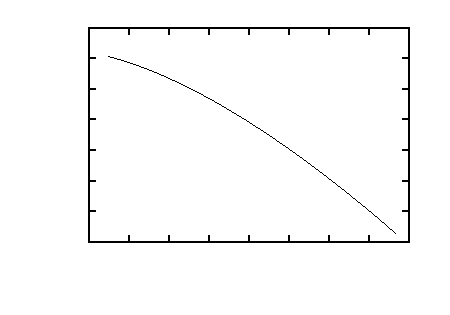
\includegraphics{chNucParamsEWater}}%
    \gplfronttext
  \end{picture}%
\endgroup
}\\
  \hspace*{-22mm}
  \subfloat[The parameter $d$ for \pfp]{% GNUPLOT: LaTeX picture with Postscript
\begingroup
  \makeatletter
  \providecommand\color[2][]{%
    \GenericError{(gnuplot) \space\space\space\@spaces}{%
      Package color not loaded in conjunction with
      terminal option `colourtext'%
    }{See the gnuplot documentation for explanation.%
    }{Either use 'blacktext' in gnuplot or load the package
      color.sty in LaTeX.}%
    \renewcommand\color[2][]{}%
  }%
  \providecommand\includegraphics[2][]{%
    \GenericError{(gnuplot) \space\space\space\@spaces}{%
      Package graphicx or graphics not loaded%
    }{See the gnuplot documentation for explanation.%
    }{The gnuplot epslatex terminal needs graphicx.sty or graphics.sty.}%
    \renewcommand\includegraphics[2][]{}%
  }%
  \providecommand\rotatebox[2]{#2}%
  \@ifundefined{ifGPcolor}{%
    \newif\ifGPcolor
    \GPcolorfalse
  }{}%
  \@ifundefined{ifGPblacktext}{%
    \newif\ifGPblacktext
    \GPblacktexttrue
  }{}%
  % define a \g@addto@macro without @ in the name:
  \let\gplgaddtomacro\g@addto@macro
  % define empty templates for all commands taking text:
  \gdef\gplbacktext{}%
  \gdef\gplfronttext{}%
  \makeatother
  \ifGPblacktext
    % no textcolor at all
    \def\colorrgb#1{}%
    \def\colorgray#1{}%
  \else
    % gray or color?
    \ifGPcolor
      \def\colorrgb#1{\color[rgb]{#1}}%
      \def\colorgray#1{\color[gray]{#1}}%
      \expandafter\def\csname LTw\endcsname{\color{white}}%
      \expandafter\def\csname LTb\endcsname{\color{black}}%
      \expandafter\def\csname LTa\endcsname{\color{black}}%
      \expandafter\def\csname LT0\endcsname{\color[rgb]{1,0,0}}%
      \expandafter\def\csname LT1\endcsname{\color[rgb]{0,1,0}}%
      \expandafter\def\csname LT2\endcsname{\color[rgb]{0,0,1}}%
      \expandafter\def\csname LT3\endcsname{\color[rgb]{1,0,1}}%
      \expandafter\def\csname LT4\endcsname{\color[rgb]{0,1,1}}%
      \expandafter\def\csname LT5\endcsname{\color[rgb]{1,1,0}}%
      \expandafter\def\csname LT6\endcsname{\color[rgb]{0,0,0}}%
      \expandafter\def\csname LT7\endcsname{\color[rgb]{1,0.3,0}}%
      \expandafter\def\csname LT8\endcsname{\color[rgb]{0.5,0.5,0.5}}%
    \else
      % gray
      \def\colorrgb#1{\color{black}}%
      \def\colorgray#1{\color[gray]{#1}}%
      \expandafter\def\csname LTw\endcsname{\color{white}}%
      \expandafter\def\csname LTb\endcsname{\color{black}}%
      \expandafter\def\csname LTa\endcsname{\color{black}}%
      \expandafter\def\csname LT0\endcsname{\color{black}}%
      \expandafter\def\csname LT1\endcsname{\color{black}}%
      \expandafter\def\csname LT2\endcsname{\color{black}}%
      \expandafter\def\csname LT3\endcsname{\color{black}}%
      \expandafter\def\csname LT4\endcsname{\color{black}}%
      \expandafter\def\csname LT5\endcsname{\color{black}}%
      \expandafter\def\csname LT6\endcsname{\color{black}}%
      \expandafter\def\csname LT7\endcsname{\color{black}}%
      \expandafter\def\csname LT8\endcsname{\color{black}}%
    \fi
  \fi
  \setlength{\unitlength}{0.0500bp}%
  \begin{picture}(4320.00,3024.00)%
    \gplgaddtomacro\gplbacktext{%
      \csname LTb\endcsname%
      \put(990,704){\makebox(0,0)[r]{\strut{} 0.595}}%
      \put(990,961){\makebox(0,0)[r]{\strut{} 0.6}}%
      \put(990,1218){\makebox(0,0)[r]{\strut{} 0.605}}%
      \put(990,1475){\makebox(0,0)[r]{\strut{} 0.61}}%
      \put(990,1732){\makebox(0,0)[r]{\strut{} 0.615}}%
      \put(990,1988){\makebox(0,0)[r]{\strut{} 0.62}}%
      \put(990,2245){\makebox(0,0)[r]{\strut{} 0.625}}%
      \put(990,2502){\makebox(0,0)[r]{\strut{} 0.63}}%
      \put(990,2759){\makebox(0,0)[r]{\strut{} 0.635}}%
      \put(1122,484){\makebox(0,0){\strut{} 200}}%
      \put(1761,484){\makebox(0,0){\strut{} 250}}%
      \put(2401,484){\makebox(0,0){\strut{} 300}}%
      \put(3040,484){\makebox(0,0){\strut{} 350}}%
      \put(3680,484){\makebox(0,0){\strut{} 400}}%
      \put(4319,484){\makebox(0,0){\strut{} 450}}%
      \put(352,1731){\rotatebox{-270}{\makebox(0,0){\strut{}$d$ ($nm$)}}}%
      \put(2720,154){\makebox(0,0){\strut{}temperature ($K$)}}%
    }%
    \gplgaddtomacro\gplfronttext{%
    }%
    \gplbacktext
    \put(0,0){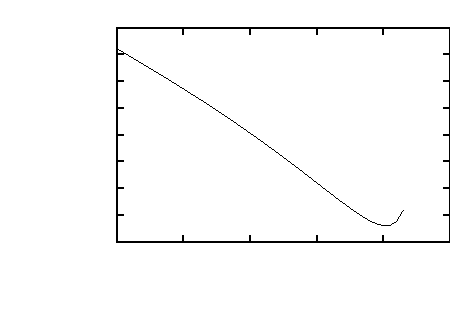
\includegraphics{chNucParamsDPfp}}%
    \gplfronttext
  \end{picture}%
\endgroup
}
  \subfloat[The parameter $\mu$ for \pfp]{% GNUPLOT: LaTeX picture with Postscript
\begingroup
  \makeatletter
  \providecommand\color[2][]{%
    \GenericError{(gnuplot) \space\space\space\@spaces}{%
      Package color not loaded in conjunction with
      terminal option `colourtext'%
    }{See the gnuplot documentation for explanation.%
    }{Either use 'blacktext' in gnuplot or load the package
      color.sty in LaTeX.}%
    \renewcommand\color[2][]{}%
  }%
  \providecommand\includegraphics[2][]{%
    \GenericError{(gnuplot) \space\space\space\@spaces}{%
      Package graphicx or graphics not loaded%
    }{See the gnuplot documentation for explanation.%
    }{The gnuplot epslatex terminal needs graphicx.sty or graphics.sty.}%
    \renewcommand\includegraphics[2][]{}%
  }%
  \providecommand\rotatebox[2]{#2}%
  \@ifundefined{ifGPcolor}{%
    \newif\ifGPcolor
    \GPcolorfalse
  }{}%
  \@ifundefined{ifGPblacktext}{%
    \newif\ifGPblacktext
    \GPblacktexttrue
  }{}%
  % define a \g@addto@macro without @ in the name:
  \let\gplgaddtomacro\g@addto@macro
  % define empty templates for all commands taking text:
  \gdef\gplbacktext{}%
  \gdef\gplfronttext{}%
  \makeatother
  \ifGPblacktext
    % no textcolor at all
    \def\colorrgb#1{}%
    \def\colorgray#1{}%
  \else
    % gray or color?
    \ifGPcolor
      \def\colorrgb#1{\color[rgb]{#1}}%
      \def\colorgray#1{\color[gray]{#1}}%
      \expandafter\def\csname LTw\endcsname{\color{white}}%
      \expandafter\def\csname LTb\endcsname{\color{black}}%
      \expandafter\def\csname LTa\endcsname{\color{black}}%
      \expandafter\def\csname LT0\endcsname{\color[rgb]{1,0,0}}%
      \expandafter\def\csname LT1\endcsname{\color[rgb]{0,1,0}}%
      \expandafter\def\csname LT2\endcsname{\color[rgb]{0,0,1}}%
      \expandafter\def\csname LT3\endcsname{\color[rgb]{1,0,1}}%
      \expandafter\def\csname LT4\endcsname{\color[rgb]{0,1,1}}%
      \expandafter\def\csname LT5\endcsname{\color[rgb]{1,1,0}}%
      \expandafter\def\csname LT6\endcsname{\color[rgb]{0,0,0}}%
      \expandafter\def\csname LT7\endcsname{\color[rgb]{1,0.3,0}}%
      \expandafter\def\csname LT8\endcsname{\color[rgb]{0.5,0.5,0.5}}%
    \else
      % gray
      \def\colorrgb#1{\color{black}}%
      \def\colorgray#1{\color[gray]{#1}}%
      \expandafter\def\csname LTw\endcsname{\color{white}}%
      \expandafter\def\csname LTb\endcsname{\color{black}}%
      \expandafter\def\csname LTa\endcsname{\color{black}}%
      \expandafter\def\csname LT0\endcsname{\color{black}}%
      \expandafter\def\csname LT1\endcsname{\color{black}}%
      \expandafter\def\csname LT2\endcsname{\color{black}}%
      \expandafter\def\csname LT3\endcsname{\color{black}}%
      \expandafter\def\csname LT4\endcsname{\color{black}}%
      \expandafter\def\csname LT5\endcsname{\color{black}}%
      \expandafter\def\csname LT6\endcsname{\color{black}}%
      \expandafter\def\csname LT7\endcsname{\color{black}}%
      \expandafter\def\csname LT8\endcsname{\color{black}}%
    \fi
  \fi
  \setlength{\unitlength}{0.0500bp}%
  \begin{picture}(4320.00,3024.00)%
    \gplgaddtomacro\gplbacktext{%
      \csname LTb\endcsname%
      \put(726,704){\makebox(0,0)[r]{\strut{}-100}}%
      \put(726,998){\makebox(0,0)[r]{\strut{}-95}}%
      \put(726,1291){\makebox(0,0)[r]{\strut{}-90}}%
      \put(726,1585){\makebox(0,0)[r]{\strut{}-85}}%
      \put(726,1878){\makebox(0,0)[r]{\strut{}-80}}%
      \put(726,2172){\makebox(0,0)[r]{\strut{}-75}}%
      \put(726,2465){\makebox(0,0)[r]{\strut{}-70}}%
      \put(726,2759){\makebox(0,0)[r]{\strut{}-65}}%
      \put(858,484){\makebox(0,0){\strut{} 200}}%
      \put(1471,484){\makebox(0,0){\strut{} 250}}%
      \put(2084,484){\makebox(0,0){\strut{} 300}}%
      \put(2697,484){\makebox(0,0){\strut{} 350}}%
      \put(3310,484){\makebox(0,0){\strut{} 400}}%
      \put(3923,484){\makebox(0,0){\strut{} 450}}%
      \put(352,1731){\rotatebox{-270}{\makebox(0,0){\strut{}$\epsilon$ ($zJ$)}}}%
      \put(2390,154){\makebox(0,0){\strut{}temperature ($K$)}}%
    }%
    \gplgaddtomacro\gplfronttext{%
    }%
    \gplbacktext
    \put(0,0){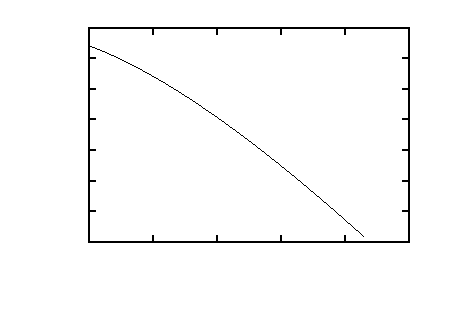
\includegraphics{chNucParamsEPfp}}%
    \gplfronttext
  \end{picture}%
\endgroup
}\\
%  \subfloat[d pfp]{\input{\missingfigure{sigma_water}}}
%  \subfloat[e pfp]{\input{\missingfigure{sigma_pfp}}}
%     \subfloat[]{
%     \missingfigure{The sketch of the arrangement}\label{fig:pressure_pulses:a}
%   }\\
  \caption{
    A plot of the  temperature dependence of the parameters $d$ and $\mu$ 
    in the hard-sphere model with Lennard-Jones interactions.
  }
 \label{fig:nuc:params}
\end{figure}

\subsubsection{The coexistence curve}

The coexistence curve for water and perfluoropentane are plotted in \figref{nuc:coex}.
The experimental values that are used to make the fit are shown with points,
and the computed curve is shown with a solid line.  
The fit for the liquid was  used to obtain $d$ and $\alpha$ for the model and so is by definition exact.
The quality of the model can be assessed by comparing the experimental values for the vapour with the fit.
It is seen to be highly accurate away from the critical point, 
at which point theory and experiment start to diverge.


The calculated spinodal is also plotted in \figref{nuc:coex}.
The spinodal defines the point of equilibrium where the energy barrier to the transition vanishes (see Favvas\cite{Favvas2008} for an introduction).
There region of the spinodal is bound by the curves
\sub{
\label{eqn:LocusSpinodal}
\begin{align}
  \mu_v = \mu_\hs(\rho_v) - \alpha \rho_v &= \mu_\hs(\rho_L) - \alpha \rho_L = \mu_L,\label{eqn:Locus0}\\
  \frac{\d \mu_v}{\d \rho} &= 0 \label{eqn:Locus1}\\
\text{or}\quad  \frac{\d \mu_L}{\d \rho} &= 0 \label{eqn:Locus2} 
\end{align}
}
Equation  \eqnref{Locus0} demands thermodynamic equilibrium.
Equation \eqnref{Locus1}  ad  \eqnref{Locus2}  demand that the equilibrium point is a saddle point (where the energy barrier vanishes).
%
%In addition to the nucleation rate we provide an upper bound on the pressure required to induce a phase change.
%The spinodal provide an upper bound on the pressure required to induce a phase change.
While the decomposition of phases past the spinodal is not  nucleation -
the phases separate throughout the medium rather than forming a bubble -
the spinodal nevertheless marks a fundamental and guaranteed  change in the medium that is surely detectable.
%It is seen that at \unit{20}\degree\ perfluoropentane will undergo a phase change at ....

The fitted values of $d$ and $\mu$ are plotted in \figref{nuc:params}.
The stability of the parameters below the critical point is encouraging
for it indicates that the predictive power of the parameters is strong.
Near the critical point the curve in 
starting to be very sensitive changes in temperature.
The model is not applicable near the critical point 
and its parameters are being pulled inappropriately by the changing 
physics.
%interactions In this domain the parameters are having 
%The parameters are b
%for it would surely indicate a failure in the model if the characteristic energy and distance 
%varied too strongly.


\ctable[cap=Density functional parameters,
        caption=Density functional parameters for perfluoropentane and water at \unit{20}\degree,
        label=table:nuc:fitparams,
        pos=top,
        %width = 0.6\textwidth,
        left
       ]
       {llrrc}
{
}{\FL
  &        & \pfp & water & 
    \ML
    &$\epsilon$  & -80 zJ &    -76 zJ   &
    \NN
    &$d$ &  \unit{0.61}\nano\metre &  \unit{0.31}\nano\metre  &
    \NN
    &$\sigma$  &  \unit{0.41}\nano\metre& \unit{0.016}\nano\metre    &   
    \LL
  }

\begin{figure}
 \centering 
  \subfloat[Density profile at the interface of water]{\label{fig:nuc:profiles:water}% GNUPLOT: LaTeX picture with Postscript
\begingroup
  \makeatletter
  \providecommand\color[2][]{%
    \GenericError{(gnuplot) \space\space\space\@spaces}{%
      Package color not loaded in conjunction with
      terminal option `colourtext'%
    }{See the gnuplot documentation for explanation.%
    }{Either use 'blacktext' in gnuplot or load the package
      color.sty in LaTeX.}%
    \renewcommand\color[2][]{}%
  }%
  \providecommand\includegraphics[2][]{%
    \GenericError{(gnuplot) \space\space\space\@spaces}{%
      Package graphicx or graphics not loaded%
    }{See the gnuplot documentation for explanation.%
    }{The gnuplot epslatex terminal needs graphicx.sty or graphics.sty.}%
    \renewcommand\includegraphics[2][]{}%
  }%
  \providecommand\rotatebox[2]{#2}%
  \@ifundefined{ifGPcolor}{%
    \newif\ifGPcolor
    \GPcolorfalse
  }{}%
  \@ifundefined{ifGPblacktext}{%
    \newif\ifGPblacktext
    \GPblacktexttrue
  }{}%
  % define a \g@addto@macro without @ in the name:
  \let\gplgaddtomacro\g@addto@macro
  % define empty templates for all commands taking text:
  \gdef\gplbacktext{}%
  \gdef\gplfronttext{}%
  \makeatother
  \ifGPblacktext
    % no textcolor at all
    \def\colorrgb#1{}%
    \def\colorgray#1{}%
  \else
    % gray or color?
    \ifGPcolor
      \def\colorrgb#1{\color[rgb]{#1}}%
      \def\colorgray#1{\color[gray]{#1}}%
      \expandafter\def\csname LTw\endcsname{\color{white}}%
      \expandafter\def\csname LTb\endcsname{\color{black}}%
      \expandafter\def\csname LTa\endcsname{\color{black}}%
      \expandafter\def\csname LT0\endcsname{\color[rgb]{1,0,0}}%
      \expandafter\def\csname LT1\endcsname{\color[rgb]{0,1,0}}%
      \expandafter\def\csname LT2\endcsname{\color[rgb]{0,0,1}}%
      \expandafter\def\csname LT3\endcsname{\color[rgb]{1,0,1}}%
      \expandafter\def\csname LT4\endcsname{\color[rgb]{0,1,1}}%
      \expandafter\def\csname LT5\endcsname{\color[rgb]{1,1,0}}%
      \expandafter\def\csname LT6\endcsname{\color[rgb]{0,0,0}}%
      \expandafter\def\csname LT7\endcsname{\color[rgb]{1,0.3,0}}%
      \expandafter\def\csname LT8\endcsname{\color[rgb]{0.5,0.5,0.5}}%
    \else
      % gray
      \def\colorrgb#1{\color{black}}%
      \def\colorgray#1{\color[gray]{#1}}%
      \expandafter\def\csname LTw\endcsname{\color{white}}%
      \expandafter\def\csname LTb\endcsname{\color{black}}%
      \expandafter\def\csname LTa\endcsname{\color{black}}%
      \expandafter\def\csname LT0\endcsname{\color{black}}%
      \expandafter\def\csname LT1\endcsname{\color{black}}%
      \expandafter\def\csname LT2\endcsname{\color{black}}%
      \expandafter\def\csname LT3\endcsname{\color{black}}%
      \expandafter\def\csname LT4\endcsname{\color{black}}%
      \expandafter\def\csname LT5\endcsname{\color{black}}%
      \expandafter\def\csname LT6\endcsname{\color{black}}%
      \expandafter\def\csname LT7\endcsname{\color{black}}%
      \expandafter\def\csname LT8\endcsname{\color{black}}%
    \fi
  \fi
  \setlength{\unitlength}{0.0500bp}%
  \begin{picture}(5760.00,4032.00)%
    \gplgaddtomacro\gplbacktext{%
      \csname LTb\endcsname%
      \put(814,704){\makebox(0,0)[r]{\strut{} 0}}%
      \put(814,1142){\makebox(0,0)[r]{\strut{} 5}}%
      \put(814,1579){\makebox(0,0)[r]{\strut{} 10}}%
      \put(814,2017){\makebox(0,0)[r]{\strut{} 15}}%
      \put(814,2454){\makebox(0,0)[r]{\strut{} 20}}%
      \put(814,2892){\makebox(0,0)[r]{\strut{} 25}}%
      \put(814,3329){\makebox(0,0)[r]{\strut{} 30}}%
      \put(814,3767){\makebox(0,0)[r]{\strut{} 35}}%
      \put(946,484){\makebox(0,0){\strut{}-4}}%
      \put(1498,484){\makebox(0,0){\strut{}-3}}%
      \put(2050,484){\makebox(0,0){\strut{}-2}}%
      \put(2602,484){\makebox(0,0){\strut{}-1}}%
      \put(3155,484){\makebox(0,0){\strut{} 0}}%
      \put(3707,484){\makebox(0,0){\strut{} 1}}%
      \put(4259,484){\makebox(0,0){\strut{} 2}}%
      \put(4811,484){\makebox(0,0){\strut{} 3}}%
      \put(5363,484){\makebox(0,0){\strut{} 4}}%
      \put(176,2235){\rotatebox{-270}{\makebox(0,0){\strut{}number density ($nm^{-3}$)}}}%
      \put(3154,154){\makebox(0,0){\strut{}distance ($nm$)}}%
    }%
    \gplgaddtomacro\gplfronttext{%
      \csname LTb\endcsname%
      \put(2266,3594){\makebox(0,0)[r]{\strut{}water}}%
      \csname LTb\endcsname%
      \put(2266,3374){\makebox(0,0)[r]{\strut{}capillary}}%
    }%
    \gplbacktext
    \put(0,0){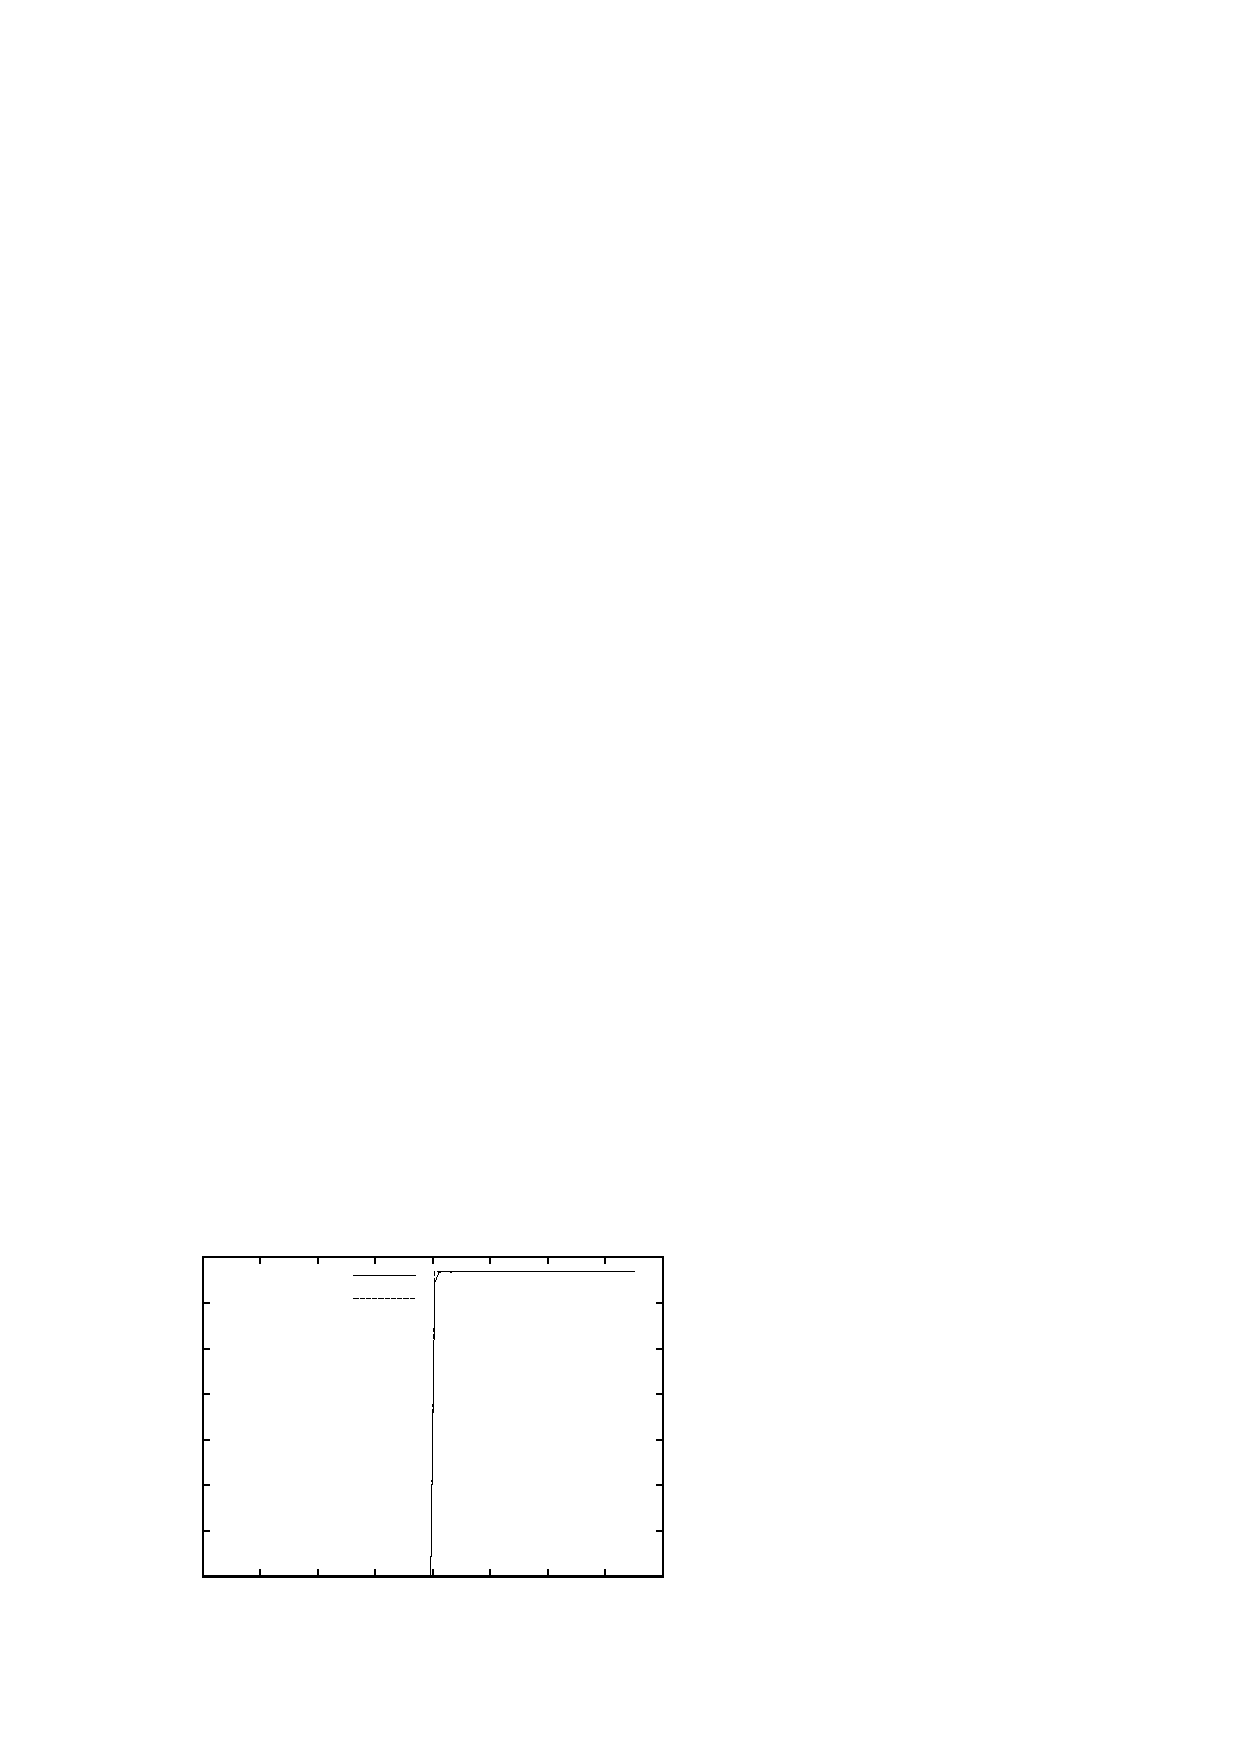
\includegraphics{profile_water}}%
    \gplfronttext
  \end{picture}%
\endgroup
}\\
  \subfloat[Density profile at the interface of \pfp]{\label{fig:nuc:profiles:pfp}% GNUPLOT: LaTeX picture with Postscript
\begingroup
  \makeatletter
  \providecommand\color[2][]{%
    \GenericError{(gnuplot) \space\space\space\@spaces}{%
      Package color not loaded in conjunction with
      terminal option `colourtext'%
    }{See the gnuplot documentation for explanation.%
    }{Either use 'blacktext' in gnuplot or load the package
      color.sty in LaTeX.}%
    \renewcommand\color[2][]{}%
  }%
  \providecommand\includegraphics[2][]{%
    \GenericError{(gnuplot) \space\space\space\@spaces}{%
      Package graphicx or graphics not loaded%
    }{See the gnuplot documentation for explanation.%
    }{The gnuplot epslatex terminal needs graphicx.sty or graphics.sty.}%
    \renewcommand\includegraphics[2][]{}%
  }%
  \providecommand\rotatebox[2]{#2}%
  \@ifundefined{ifGPcolor}{%
    \newif\ifGPcolor
    \GPcolorfalse
  }{}%
  \@ifundefined{ifGPblacktext}{%
    \newif\ifGPblacktext
    \GPblacktexttrue
  }{}%
  % define a \g@addto@macro without @ in the name:
  \let\gplgaddtomacro\g@addto@macro
  % define empty templates for all commands taking text:
  \gdef\gplbacktext{}%
  \gdef\gplfronttext{}%
  \makeatother
  \ifGPblacktext
    % no textcolor at all
    \def\colorrgb#1{}%
    \def\colorgray#1{}%
  \else
    % gray or color?
    \ifGPcolor
      \def\colorrgb#1{\color[rgb]{#1}}%
      \def\colorgray#1{\color[gray]{#1}}%
      \expandafter\def\csname LTw\endcsname{\color{white}}%
      \expandafter\def\csname LTb\endcsname{\color{black}}%
      \expandafter\def\csname LTa\endcsname{\color{black}}%
      \expandafter\def\csname LT0\endcsname{\color[rgb]{1,0,0}}%
      \expandafter\def\csname LT1\endcsname{\color[rgb]{0,1,0}}%
      \expandafter\def\csname LT2\endcsname{\color[rgb]{0,0,1}}%
      \expandafter\def\csname LT3\endcsname{\color[rgb]{1,0,1}}%
      \expandafter\def\csname LT4\endcsname{\color[rgb]{0,1,1}}%
      \expandafter\def\csname LT5\endcsname{\color[rgb]{1,1,0}}%
      \expandafter\def\csname LT6\endcsname{\color[rgb]{0,0,0}}%
      \expandafter\def\csname LT7\endcsname{\color[rgb]{1,0.3,0}}%
      \expandafter\def\csname LT8\endcsname{\color[rgb]{0.5,0.5,0.5}}%
    \else
      % gray
      \def\colorrgb#1{\color{black}}%
      \def\colorgray#1{\color[gray]{#1}}%
      \expandafter\def\csname LTw\endcsname{\color{white}}%
      \expandafter\def\csname LTb\endcsname{\color{black}}%
      \expandafter\def\csname LTa\endcsname{\color{black}}%
      \expandafter\def\csname LT0\endcsname{\color{black}}%
      \expandafter\def\csname LT1\endcsname{\color{black}}%
      \expandafter\def\csname LT2\endcsname{\color{black}}%
      \expandafter\def\csname LT3\endcsname{\color{black}}%
      \expandafter\def\csname LT4\endcsname{\color{black}}%
      \expandafter\def\csname LT5\endcsname{\color{black}}%
      \expandafter\def\csname LT6\endcsname{\color{black}}%
      \expandafter\def\csname LT7\endcsname{\color{black}}%
      \expandafter\def\csname LT8\endcsname{\color{black}}%
    \fi
  \fi
  \setlength{\unitlength}{0.0500bp}%
  \begin{picture}(5760.00,4032.00)%
    \gplgaddtomacro\gplbacktext{%
      \csname LTb\endcsname%
      \put(946,704){\makebox(0,0)[r]{\strut{} 0}}%
      \put(946,1044){\makebox(0,0)[r]{\strut{} 0.5}}%
      \put(946,1385){\makebox(0,0)[r]{\strut{} 1}}%
      \put(946,1725){\makebox(0,0)[r]{\strut{} 1.5}}%
      \put(946,2065){\makebox(0,0)[r]{\strut{} 2}}%
      \put(946,2406){\makebox(0,0)[r]{\strut{} 2.5}}%
      \put(946,2746){\makebox(0,0)[r]{\strut{} 3}}%
      \put(946,3086){\makebox(0,0)[r]{\strut{} 3.5}}%
      \put(946,3427){\makebox(0,0)[r]{\strut{} 4}}%
      \put(946,3767){\makebox(0,0)[r]{\strut{} 4.5}}%
      \put(1078,484){\makebox(0,0){\strut{}-4}}%
      \put(1614,484){\makebox(0,0){\strut{}-3}}%
      \put(2149,484){\makebox(0,0){\strut{}-2}}%
      \put(2685,484){\makebox(0,0){\strut{}-1}}%
      \put(3221,484){\makebox(0,0){\strut{} 0}}%
      \put(3756,484){\makebox(0,0){\strut{} 1}}%
      \put(4292,484){\makebox(0,0){\strut{} 2}}%
      \put(4827,484){\makebox(0,0){\strut{} 3}}%
      \put(5363,484){\makebox(0,0){\strut{} 4}}%
      \put(176,2235){\rotatebox{-270}{\makebox(0,0){\strut{}number density ($nm^{-3}$)}}}%
      \put(3220,154){\makebox(0,0){\strut{}distance ($nm$)}}%
    }%
    \gplgaddtomacro\gplfronttext{%
      \csname LTb\endcsname%
      \put(2398,3594){\makebox(0,0)[r]{\strut{}pfp}}%
      \csname LTb\endcsname%
      \put(2398,3374){\makebox(0,0)[r]{\strut{}capillary}}%
    }%
    \gplbacktext
    \put(0,0){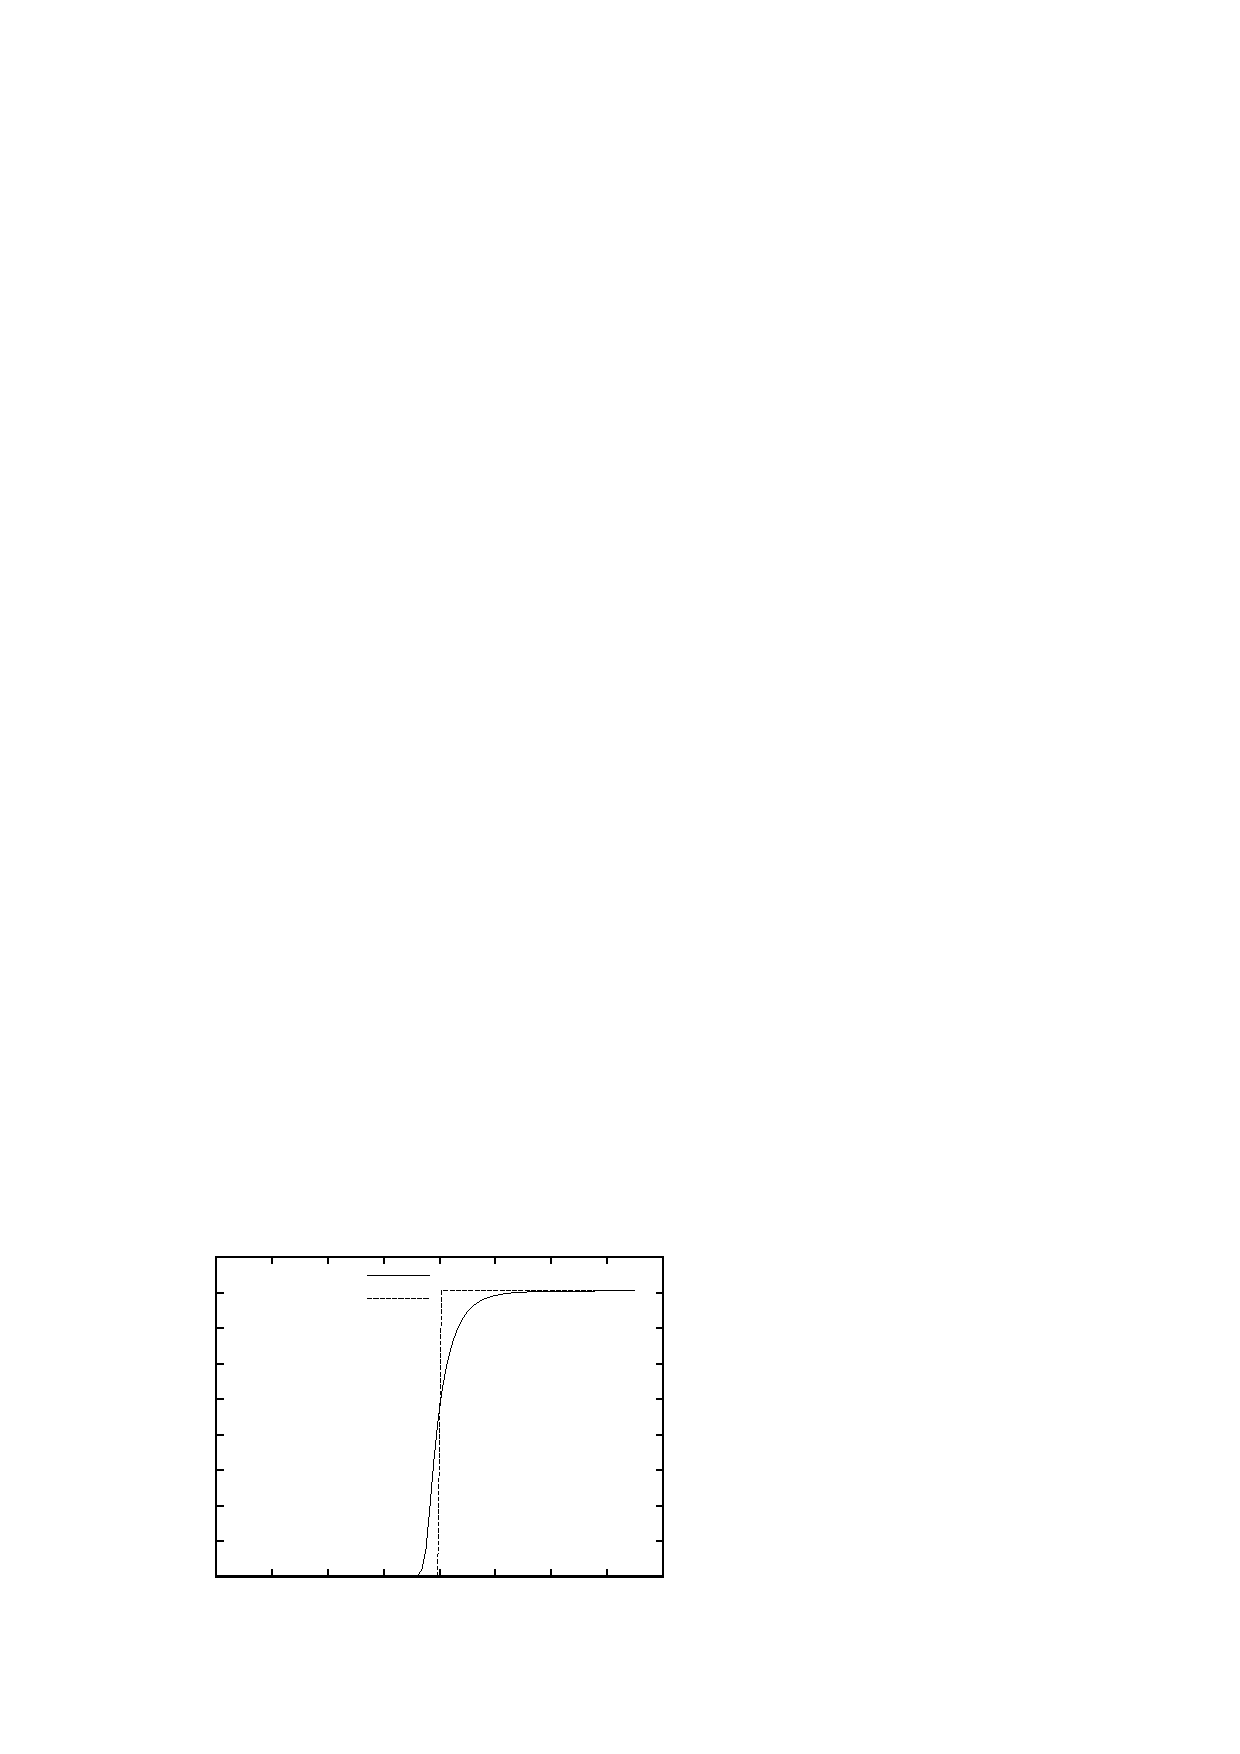
\includegraphics{profile_pfp}}%
    \gplfronttext
  \end{picture}%
\endgroup
}
\caption{
    The plainer density profiles of water and perfluoropentane at \unit{293}\kelvin.
  }
 \label{fig:nuc:profiles}
\end{figure}



The parameters at \unit{20}\degree\ are plotted in \tabref{nuc:fitparams}.
One notable observation is that the distance scale in the Lennard-Jones model is very small for water.
This indicates a very low interaction length. %, which is illustrated in \figref{nuc:LennardJones}.
The reason for this is the highly polar nature of water.
Density functional approaches have previously been found to struggle in the presence of highly polar fluids such as water\cite{Talanquer2001, Nyquist1995},
with the same consequence for the value of $d$.

In \figref{nuc:profiles}
the density profiles for water and perfluoropentane are plotted.
The small value of $d$ for water means that the 
density profile varies over very rapidly 
and is essentially indistinguishable from the capillary approximation.
%The are box expected to perform equally poorly.

From \figref{nuc:profiles:pfp} it is seen that the density profile for \pfp\ varies over a more significant length scale.
The \unit{1}\nano\metre\ of \figref{nuc:profiles:pfp} represents approximately 10\%
of the critical radius of a \pfp\ vapour droplet under \unit{1}\mega\pascal\ tension.
The use of the  capillary approximation for \pfp\ is therefore highly questionable.








%However, Talanquer and Oxtoby used dissolved gasses such as oxygen and carbon dioxide as their examples of nucleation. 
%The high vapour pressures of these gases causes the critical radius of the bubble very small: just a few na
%with a corresponding  cause considered  the nucleation of highly volatile liquids  the nucleaton of volatile liquids 

%Such spectacular deviations are typical for bubble nucleation predictions. 
%On the other hand, for predicting the condensation of a vapour bubble 
%\cnt\ is often satisfactory.
%The density functional approach explained this discrepancy by finding that the 
%spinodal exerts a stronger influence on the liquid-vapour transition than its reverse\cite{Oxtoby1997}.
%\Cnt\ does not model the spinodal and the rates predicted for   evaporation and condensation are identical.
%The qualitative success of the classical theory for this transition was considered fortuitous,
%resulting from a cancellation of errors\cite{Oxtoby1997}.

%Talanquer and Oxtoby, however,



%\subsubsection{The density profile}

%\subsection{Evaluation of the Capillary approximation}

\subsection{Further work}
The density profile of \pfp\ plotted in \figref{nuc:profiles:pfp}
indicates that the density functional approach may 
have much to offer theoretical studies of perfluoropentane.

In particular, the density functional approach can be
extended to binary fluids\cite{Talanquer2001} to estimate the nucleation rates for various 
gases dissolved within the perfluorpentane droplet.
The perfluorocarbons are remarkable for their solubility of carbon dioxide.
It could be that type 1  nucleation can be facilitated by the perfluorocarbons  
not by  their low boiling points,
but rather due to the nucleation of their dissolved gases.
%of the medium, but due to the ease with which their solutes form 

\hl{One word of caution.}
  The density functional approach is a mean field technique that fails near the critical temperature.
  We have argued that the critical temperatures of perfluorobutane and perfluoropentane are sufficiently high that the super heat limits of these materials do not come into play.
  Recent experimental evidence from  Mountford\cite{Mountford2015} found that vapourisation of perfluorobutane occurred at \unit{75}\degreecelsius, uncomfortably close to the limit of  \unit{113}\degreecelsius\ for the purpose of a mean field approach. 
  This work, however, did not use ultrasound to induce phase changes in the medium, and so the super-harmonic focussing found by Shpak\cite{Shpak2014} to be so influential was not available. 



%  (using the coexistence value of $\mu$)

%which is plotted in \figref{sppressure}
% Below the critical temperature two phases exist and so the simultaneous  equations \eqnref{BulkCoex} can be solved numerically 
% so long as  $p_\hs(rho)$ and $\mu(\rho)$ are known functions of $\rho$.
% The solutions to \eqnref{BulkCoex} as a function of temperature define the coexistence curve.
%Each minima 

%There is a degree of ambiguity as to what the choice of $d$ should be.
%One choice could be hard sphere diameter of the Kihira model.
%However, as seen from \figref{Kihira_d}, 
%this choice seems unrepresentatively small.
%A more appropriate looking choice seems to be the characteristic length $\sigma$.

%To overcome this difficulty the data is fitted to the


% \begin{figure}
%  \centering
% %\hspace*{-0.2cm}
% % \label{fig:Kihira_potentials}
%  \subfloat[Kihira 2-particle potentials for various perfluorocarbons]{
%   % GNUPLOT: LaTeX picture with Postscript
\begingroup
  \makeatletter
  \providecommand\color[2][]{%
    \GenericError{(gnuplot) \space\space\space\@spaces}{%
      Package color not loaded in conjunction with
      terminal option `colourtext'%
    }{See the gnuplot documentation for explanation.%
    }{Either use 'blacktext' in gnuplot or load the package
      color.sty in LaTeX.}%
    \renewcommand\color[2][]{}%
  }%
  \providecommand\includegraphics[2][]{%
    \GenericError{(gnuplot) \space\space\space\@spaces}{%
      Package graphicx or graphics not loaded%
    }{See the gnuplot documentation for explanation.%
    }{The gnuplot epslatex terminal needs graphicx.sty or graphics.sty.}%
    \renewcommand\includegraphics[2][]{}%
  }%
  \providecommand\rotatebox[2]{#2}%
  \@ifundefined{ifGPcolor}{%
    \newif\ifGPcolor
    \GPcolorfalse
  }{}%
  \@ifundefined{ifGPblacktext}{%
    \newif\ifGPblacktext
    \GPblacktexttrue
  }{}%
  % define a \g@addto@macro without @ in the name:
  \let\gplgaddtomacro\g@addto@macro
  % define empty templates for all commands taking text:
  \gdef\gplbacktext{}%
  \gdef\gplfronttext{}%
  \makeatother
  \ifGPblacktext
    % no textcolor at all
    \def\colorrgb#1{}%
    \def\colorgray#1{}%
  \else
    % gray or color?
    \ifGPcolor
      \def\colorrgb#1{\color[rgb]{#1}}%
      \def\colorgray#1{\color[gray]{#1}}%
      \expandafter\def\csname LTw\endcsname{\color{white}}%
      \expandafter\def\csname LTb\endcsname{\color{black}}%
      \expandafter\def\csname LTa\endcsname{\color{black}}%
      \expandafter\def\csname LT0\endcsname{\color[rgb]{1,0,0}}%
      \expandafter\def\csname LT1\endcsname{\color[rgb]{0,1,0}}%
      \expandafter\def\csname LT2\endcsname{\color[rgb]{0,0,1}}%
      \expandafter\def\csname LT3\endcsname{\color[rgb]{1,0,1}}%
      \expandafter\def\csname LT4\endcsname{\color[rgb]{0,1,1}}%
      \expandafter\def\csname LT5\endcsname{\color[rgb]{1,1,0}}%
      \expandafter\def\csname LT6\endcsname{\color[rgb]{0,0,0}}%
      \expandafter\def\csname LT7\endcsname{\color[rgb]{1,0.3,0}}%
      \expandafter\def\csname LT8\endcsname{\color[rgb]{0.5,0.5,0.5}}%
    \else
      % gray
      \def\colorrgb#1{\color{black}}%
      \def\colorgray#1{\color[gray]{#1}}%
      \expandafter\def\csname LTw\endcsname{\color{white}}%
      \expandafter\def\csname LTb\endcsname{\color{black}}%
      \expandafter\def\csname LTa\endcsname{\color{black}}%
      \expandafter\def\csname LT0\endcsname{\color{black}}%
      \expandafter\def\csname LT1\endcsname{\color{black}}%
      \expandafter\def\csname LT2\endcsname{\color{black}}%
      \expandafter\def\csname LT3\endcsname{\color{black}}%
      \expandafter\def\csname LT4\endcsname{\color{black}}%
      \expandafter\def\csname LT5\endcsname{\color{black}}%
      \expandafter\def\csname LT6\endcsname{\color{black}}%
      \expandafter\def\csname LT7\endcsname{\color{black}}%
      \expandafter\def\csname LT8\endcsname{\color{black}}%
    \fi
  \fi
  \setlength{\unitlength}{0.0500bp}%
  \begin{picture}(5040.00,3528.00)%
    \gplgaddtomacro\gplbacktext{%
      \csname LTb\endcsname%
      \put(1210,704){\makebox(0,0)[r]{\strut{} 0}}%
      \put(1210,1070){\makebox(0,0)[r]{\strut{} 0.5}}%
      \put(1210,1435){\makebox(0,0)[r]{\strut{} 1}}%
      \put(1210,1801){\makebox(0,0)[r]{\strut{} 1.5}}%
      \put(1210,2167){\makebox(0,0)[r]{\strut{} 2}}%
      \put(1210,2533){\makebox(0,0)[r]{\strut{} 2.5}}%
      \put(1210,2898){\makebox(0,0)[r]{\strut{} 3}}%
      \put(1210,3264){\makebox(0,0)[r]{\strut{} 3.5}}%
      \put(1342,484){\makebox(0,0){\strut{} 200}}%
      \put(1791,484){\makebox(0,0){\strut{} 220}}%
      \put(2240,484){\makebox(0,0){\strut{} 240}}%
      \put(2689,484){\makebox(0,0){\strut{} 260}}%
      \put(3138,484){\makebox(0,0){\strut{} 280}}%
      \put(3587,484){\makebox(0,0){\strut{} 300}}%
      \put(4036,484){\makebox(0,0){\strut{} 320}}%
      \put(4485,484){\makebox(0,0){\strut{} 340}}%
      \put(440,1984){\rotatebox{90}{\makebox(0,0){\strut{}vapour pressure, atm}}}%
      \put(3026,154){\makebox(0,0){\strut{}temperature, K}}%
    }%
    \gplgaddtomacro\gplfronttext{%
      \csname LTb\endcsname%
      \put(3058,3091){\makebox(0,0)[r]{\strut{}fit}}%
      \csname LTb\endcsname%
      \put(3058,2871){\makebox(0,0)[r]{\strut{}Barber 1955}}%
      \csname LTb\endcsname%
      \put(3058,2651){\makebox(0,0)[r]{\strut{}Crowder 1967}}%
    }%
    \gplbacktext
    \put(0,0){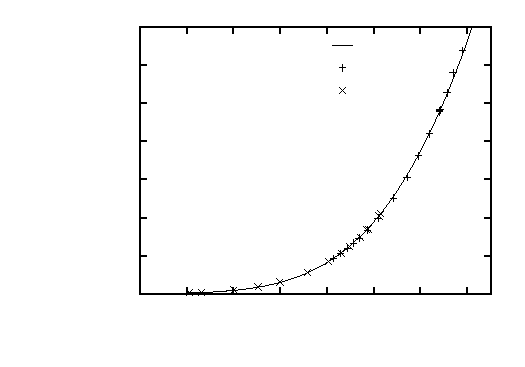
\includegraphics{c2_vapour_pressure_fit}}%
    \gplfronttext
  \end{picture}%
\endgroup
}
% \hfill
% % \label{fig:Kihira_WCA}
%  \subfloat[WCA decomposition of the Kihira  potential for perfluoropentane]{
%   % GNUPLOT: LaTeX picture with Postscript
\begingroup
  \makeatletter
  \providecommand\color[2][]{%
    \GenericError{(gnuplot) \space\space\space\@spaces}{%
      Package color not loaded in conjunction with
      terminal option `colourtext'%
    }{See the gnuplot documentation for explanation.%
    }{Either use 'blacktext' in gnuplot or load the package
      color.sty in LaTeX.}%
    \renewcommand\color[2][]{}%
  }%
  \providecommand\includegraphics[2][]{%
    \GenericError{(gnuplot) \space\space\space\@spaces}{%
      Package graphicx or graphics not loaded%
    }{See the gnuplot documentation for explanation.%
    }{The gnuplot epslatex terminal needs graphicx.sty or graphics.sty.}%
    \renewcommand\includegraphics[2][]{}%
  }%
  \providecommand\rotatebox[2]{#2}%
  \@ifundefined{ifGPcolor}{%
    \newif\ifGPcolor
    \GPcolorfalse
  }{}%
  \@ifundefined{ifGPblacktext}{%
    \newif\ifGPblacktext
    \GPblacktexttrue
  }{}%
  % define a \g@addto@macro without @ in the name:
  \let\gplgaddtomacro\g@addto@macro
  % define empty templates for all commands taking text:
  \gdef\gplbacktext{}%
  \gdef\gplfronttext{}%
  \makeatother
  \ifGPblacktext
    % no textcolor at all
    \def\colorrgb#1{}%
    \def\colorgray#1{}%
  \else
    % gray or color?
    \ifGPcolor
      \def\colorrgb#1{\color[rgb]{#1}}%
      \def\colorgray#1{\color[gray]{#1}}%
      \expandafter\def\csname LTw\endcsname{\color{white}}%
      \expandafter\def\csname LTb\endcsname{\color{black}}%
      \expandafter\def\csname LTa\endcsname{\color{black}}%
      \expandafter\def\csname LT0\endcsname{\color[rgb]{1,0,0}}%
      \expandafter\def\csname LT1\endcsname{\color[rgb]{0,1,0}}%
      \expandafter\def\csname LT2\endcsname{\color[rgb]{0,0,1}}%
      \expandafter\def\csname LT3\endcsname{\color[rgb]{1,0,1}}%
      \expandafter\def\csname LT4\endcsname{\color[rgb]{0,1,1}}%
      \expandafter\def\csname LT5\endcsname{\color[rgb]{1,1,0}}%
      \expandafter\def\csname LT6\endcsname{\color[rgb]{0,0,0}}%
      \expandafter\def\csname LT7\endcsname{\color[rgb]{1,0.3,0}}%
      \expandafter\def\csname LT8\endcsname{\color[rgb]{0.5,0.5,0.5}}%
    \else
      % gray
      \def\colorrgb#1{\color{black}}%
      \def\colorgray#1{\color[gray]{#1}}%
      \expandafter\def\csname LTw\endcsname{\color{white}}%
      \expandafter\def\csname LTb\endcsname{\color{black}}%
      \expandafter\def\csname LTa\endcsname{\color{black}}%
      \expandafter\def\csname LT0\endcsname{\color{black}}%
      \expandafter\def\csname LT1\endcsname{\color{black}}%
      \expandafter\def\csname LT2\endcsname{\color{black}}%
      \expandafter\def\csname LT3\endcsname{\color{black}}%
      \expandafter\def\csname LT4\endcsname{\color{black}}%
      \expandafter\def\csname LT5\endcsname{\color{black}}%
      \expandafter\def\csname LT6\endcsname{\color{black}}%
      \expandafter\def\csname LT7\endcsname{\color{black}}%
      \expandafter\def\csname LT8\endcsname{\color{black}}%
    \fi
  \fi
  \setlength{\unitlength}{0.0500bp}%
  \begin{picture}(5040.00,3528.00)%
    \gplgaddtomacro\gplbacktext{%
      \csname LTb\endcsname%
      \put(1210,704){\makebox(0,0)[r]{\strut{} 0}}%
      \put(1210,1070){\makebox(0,0)[r]{\strut{} 0.5}}%
      \put(1210,1435){\makebox(0,0)[r]{\strut{} 1}}%
      \put(1210,1801){\makebox(0,0)[r]{\strut{} 1.5}}%
      \put(1210,2167){\makebox(0,0)[r]{\strut{} 2}}%
      \put(1210,2533){\makebox(0,0)[r]{\strut{} 2.5}}%
      \put(1210,2898){\makebox(0,0)[r]{\strut{} 3}}%
      \put(1210,3264){\makebox(0,0)[r]{\strut{} 3.5}}%
      \put(1342,484){\makebox(0,0){\strut{} 200}}%
      \put(1791,484){\makebox(0,0){\strut{} 220}}%
      \put(2240,484){\makebox(0,0){\strut{} 240}}%
      \put(2689,484){\makebox(0,0){\strut{} 260}}%
      \put(3138,484){\makebox(0,0){\strut{} 280}}%
      \put(3587,484){\makebox(0,0){\strut{} 300}}%
      \put(4036,484){\makebox(0,0){\strut{} 320}}%
      \put(4485,484){\makebox(0,0){\strut{} 340}}%
      \put(440,1984){\rotatebox{90}{\makebox(0,0){\strut{}vapour pressure, atm}}}%
      \put(3026,154){\makebox(0,0){\strut{}temperature, K}}%
    }%
    \gplgaddtomacro\gplfronttext{%
      \csname LTb\endcsname%
      \put(3058,3091){\makebox(0,0)[r]{\strut{}fit}}%
      \csname LTb\endcsname%
      \put(3058,2871){\makebox(0,0)[r]{\strut{}Barber 1955}}%
      \csname LTb\endcsname%
      \put(3058,2651){\makebox(0,0)[r]{\strut{}Crowder 1967}}%
    }%
    \gplbacktext
    \put(0,0){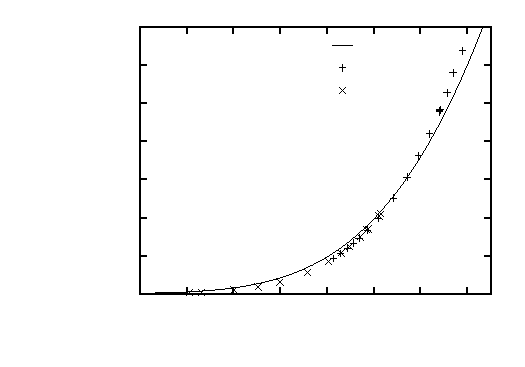
\includegraphics{c2_vapour_pressure_fit_LJ}}%
    \gplfronttext
  \end{picture}%
\endgroup
}\\
% %\label{fig:Kihira_d}
%   \caption{ 
%   }
%  \label{fig:}
% \end{figure}

%The final result of the density functional approach, \figref{profile} shows that the thickness of the interface extends over 10 anstrums on each side of the inteface.
%xsThis is extends over most of the bubble wheWhen this compared to the



% \begin{figure}
%  \centering
% %\hspace*{-0.2cm}
%   % GNUPLOT: LaTeX picture with Postscript
\begingroup
  \makeatletter
  \providecommand\color[2][]{%
    \GenericError{(gnuplot) \space\space\space\@spaces}{%
      Package color not loaded in conjunction with
      terminal option `colourtext'%
    }{See the gnuplot documentation for explanation.%
    }{Either use 'blacktext' in gnuplot or load the package
      color.sty in LaTeX.}%
    \renewcommand\color[2][]{}%
  }%
  \providecommand\includegraphics[2][]{%
    \GenericError{(gnuplot) \space\space\space\@spaces}{%
      Package graphicx or graphics not loaded%
    }{See the gnuplot documentation for explanation.%
    }{The gnuplot epslatex terminal needs graphicx.sty or graphics.sty.}%
    \renewcommand\includegraphics[2][]{}%
  }%
  \providecommand\rotatebox[2]{#2}%
  \@ifundefined{ifGPcolor}{%
    \newif\ifGPcolor
    \GPcolorfalse
  }{}%
  \@ifundefined{ifGPblacktext}{%
    \newif\ifGPblacktext
    \GPblacktexttrue
  }{}%
  % define a \g@addto@macro without @ in the name:
  \let\gplgaddtomacro\g@addto@macro
  % define empty templates for all commands taking text:
  \gdef\gplbacktext{}%
  \gdef\gplfronttext{}%
  \makeatother
  \ifGPblacktext
    % no textcolor at all
    \def\colorrgb#1{}%
    \def\colorgray#1{}%
  \else
    % gray or color?
    \ifGPcolor
      \def\colorrgb#1{\color[rgb]{#1}}%
      \def\colorgray#1{\color[gray]{#1}}%
      \expandafter\def\csname LTw\endcsname{\color{white}}%
      \expandafter\def\csname LTb\endcsname{\color{black}}%
      \expandafter\def\csname LTa\endcsname{\color{black}}%
      \expandafter\def\csname LT0\endcsname{\color[rgb]{1,0,0}}%
      \expandafter\def\csname LT1\endcsname{\color[rgb]{0,1,0}}%
      \expandafter\def\csname LT2\endcsname{\color[rgb]{0,0,1}}%
      \expandafter\def\csname LT3\endcsname{\color[rgb]{1,0,1}}%
      \expandafter\def\csname LT4\endcsname{\color[rgb]{0,1,1}}%
      \expandafter\def\csname LT5\endcsname{\color[rgb]{1,1,0}}%
      \expandafter\def\csname LT6\endcsname{\color[rgb]{0,0,0}}%
      \expandafter\def\csname LT7\endcsname{\color[rgb]{1,0.3,0}}%
      \expandafter\def\csname LT8\endcsname{\color[rgb]{0.5,0.5,0.5}}%
    \else
      % gray
      \def\colorrgb#1{\color{black}}%
      \def\colorgray#1{\color[gray]{#1}}%
      \expandafter\def\csname LTw\endcsname{\color{white}}%
      \expandafter\def\csname LTb\endcsname{\color{black}}%
      \expandafter\def\csname LTa\endcsname{\color{black}}%
      \expandafter\def\csname LT0\endcsname{\color{black}}%
      \expandafter\def\csname LT1\endcsname{\color{black}}%
      \expandafter\def\csname LT2\endcsname{\color{black}}%
      \expandafter\def\csname LT3\endcsname{\color{black}}%
      \expandafter\def\csname LT4\endcsname{\color{black}}%
      \expandafter\def\csname LT5\endcsname{\color{black}}%
      \expandafter\def\csname LT6\endcsname{\color{black}}%
      \expandafter\def\csname LT7\endcsname{\color{black}}%
      \expandafter\def\csname LT8\endcsname{\color{black}}%
    \fi
  \fi
  \setlength{\unitlength}{0.0500bp}%
  \begin{picture}(5040.00,3528.00)%
    \gplgaddtomacro\gplbacktext{%
      \csname LTb\endcsname%
      \put(1606,704){\makebox(0,0)[r]{\strut{} 0}}%
      \put(1606,1070){\makebox(0,0)[r]{\strut{} 0.0005}}%
      \put(1606,1435){\makebox(0,0)[r]{\strut{} 0.001}}%
      \put(1606,1801){\makebox(0,0)[r]{\strut{} 0.0015}}%
      \put(1606,2167){\makebox(0,0)[r]{\strut{} 0.002}}%
      \put(1606,2533){\makebox(0,0)[r]{\strut{} 0.0025}}%
      \put(1606,2898){\makebox(0,0)[r]{\strut{} 0.003}}%
      \put(1606,3264){\makebox(0,0)[r]{\strut{} 0.0035}}%
      \put(1738,484){\makebox(0,0){\strut{} 0}}%
      \put(2233,484){\makebox(0,0){\strut{} 20}}%
      \put(2729,484){\makebox(0,0){\strut{} 40}}%
      \put(3224,484){\makebox(0,0){\strut{} 60}}%
      \put(3719,484){\makebox(0,0){\strut{} 80}}%
      \put(4215,484){\makebox(0,0){\strut{} 100}}%
      \put(4710,484){\makebox(0,0){\strut{} 120}}%
      \put(440,1984){\rotatebox{90}{\makebox(0,0){\strut{}number density}}}%
      \put(3224,154){\makebox(0,0){\strut{}distance, Angstrum}}%
    }%
    \gplgaddtomacro\gplfronttext{%
    }%
    \gplbacktext
    \put(0,0){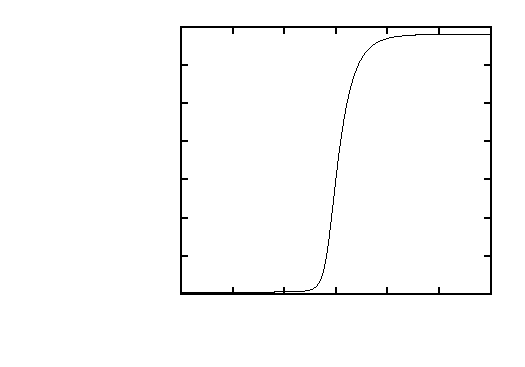
\includegraphics{c2_interface}}%
    \gplfronttext
  \end{picture}%
\endgroup

%   \caption{ The density profile of perfluoropentane at a plainer interface.
%   }
%  \label{fig:profile}
% \end{figure}
% \begin{figure}
%   % GNUPLOT: LaTeX picture with Postscript
\begingroup
  \makeatletter
  \providecommand\color[2][]{%
    \GenericError{(gnuplot) \space\space\space\@spaces}{%
      Package color not loaded in conjunction with
      terminal option `colourtext'%
    }{See the gnuplot documentation for explanation.%
    }{Either use 'blacktext' in gnuplot or load the package
      color.sty in LaTeX.}%
    \renewcommand\color[2][]{}%
  }%
  \providecommand\includegraphics[2][]{%
    \GenericError{(gnuplot) \space\space\space\@spaces}{%
      Package graphicx or graphics not loaded%
    }{See the gnuplot documentation for explanation.%
    }{The gnuplot epslatex terminal needs graphicx.sty or graphics.sty.}%
    \renewcommand\includegraphics[2][]{}%
  }%
  \providecommand\rotatebox[2]{#2}%
  \@ifundefined{ifGPcolor}{%
    \newif\ifGPcolor
    \GPcolorfalse
  }{}%
  \@ifundefined{ifGPblacktext}{%
    \newif\ifGPblacktext
    \GPblacktexttrue
  }{}%
  % define a \g@addto@macro without @ in the name:
  \let\gplgaddtomacro\g@addto@macro
  % define empty templates for all commands taking text:
  \gdef\gplbacktext{}%
  \gdef\gplfronttext{}%
  \makeatother
  \ifGPblacktext
    % no textcolor at all
    \def\colorrgb#1{}%
    \def\colorgray#1{}%
  \else
    % gray or color?
    \ifGPcolor
      \def\colorrgb#1{\color[rgb]{#1}}%
      \def\colorgray#1{\color[gray]{#1}}%
      \expandafter\def\csname LTw\endcsname{\color{white}}%
      \expandafter\def\csname LTb\endcsname{\color{black}}%
      \expandafter\def\csname LTa\endcsname{\color{black}}%
      \expandafter\def\csname LT0\endcsname{\color[rgb]{1,0,0}}%
      \expandafter\def\csname LT1\endcsname{\color[rgb]{0,1,0}}%
      \expandafter\def\csname LT2\endcsname{\color[rgb]{0,0,1}}%
      \expandafter\def\csname LT3\endcsname{\color[rgb]{1,0,1}}%
      \expandafter\def\csname LT4\endcsname{\color[rgb]{0,1,1}}%
      \expandafter\def\csname LT5\endcsname{\color[rgb]{1,1,0}}%
      \expandafter\def\csname LT6\endcsname{\color[rgb]{0,0,0}}%
      \expandafter\def\csname LT7\endcsname{\color[rgb]{1,0.3,0}}%
      \expandafter\def\csname LT8\endcsname{\color[rgb]{0.5,0.5,0.5}}%
    \else
      % gray
      \def\colorrgb#1{\color{black}}%
      \def\colorgray#1{\color[gray]{#1}}%
      \expandafter\def\csname LTw\endcsname{\color{white}}%
      \expandafter\def\csname LTb\endcsname{\color{black}}%
      \expandafter\def\csname LTa\endcsname{\color{black}}%
      \expandafter\def\csname LT0\endcsname{\color{black}}%
      \expandafter\def\csname LT1\endcsname{\color{black}}%
      \expandafter\def\csname LT2\endcsname{\color{black}}%
      \expandafter\def\csname LT3\endcsname{\color{black}}%
      \expandafter\def\csname LT4\endcsname{\color{black}}%
      \expandafter\def\csname LT5\endcsname{\color{black}}%
      \expandafter\def\csname LT6\endcsname{\color{black}}%
      \expandafter\def\csname LT7\endcsname{\color{black}}%
      \expandafter\def\csname LT8\endcsname{\color{black}}%
    \fi
  \fi
  \setlength{\unitlength}{0.0500bp}%
  \begin{picture}(5040.00,3528.00)%
    \gplgaddtomacro\gplbacktext{%
      \csname LTb\endcsname%
      \put(1078,704){\makebox(0,0)[r]{\strut{} 0}}%
      \put(1078,1216){\makebox(0,0)[r]{\strut{} 10}}%
      \put(1078,1728){\makebox(0,0)[r]{\strut{} 20}}%
      \put(1078,2240){\makebox(0,0)[r]{\strut{} 30}}%
      \put(1078,2752){\makebox(0,0)[r]{\strut{} 40}}%
      \put(1078,3264){\makebox(0,0)[r]{\strut{} 50}}%
      \put(1210,484){\makebox(0,0){\strut{} 200}}%
      \put(1910,484){\makebox(0,0){\strut{} 250}}%
      \put(2610,484){\makebox(0,0){\strut{} 300}}%
      \put(3310,484){\makebox(0,0){\strut{} 350}}%
      \put(4010,484){\makebox(0,0){\strut{} 400}}%
      \put(4710,484){\makebox(0,0){\strut{} 450}}%
      \put(440,1984){\rotatebox{90}{\makebox(0,0){\strut{}pressure (MPa)}}}%
      \put(2960,154){\makebox(0,0){\strut{}temperature, K}}%
    }%
    \gplgaddtomacro\gplfronttext{%
    }%
    \gplbacktext
    \put(0,0){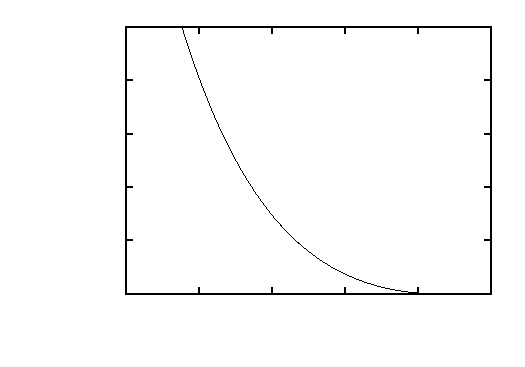
\includegraphics{c2_lspinodal_pressure}}%
    \gplfronttext
  \end{picture}%
\endgroup

%   \caption{ 
%     The pressure difference between coexistence and the liquid spinodal.
% This graph calculates  the pressures required to guarantee a phase change.
% Notice that the pressures required vanish at the critical pressure.
%   }
%  \label{fig:sppressure}
% \end{figure}



% \subsubsection{The Carnarhan-Stirling Hard Sphere Equation of State}


% To make further progress we need to solve the thermodynamics of the reference hard sphere fluid.
% This can be done by starting with the hightly accurate Carnahan-Stirling equaion of state,
% Carnahan-Starling\cite{Carnahan1969} see\cite{Song1989} for interest, equation of state
% \begin{align}
% Z = \frac{pV}{N\kB T} = \frac{1+\eta +\eta^2-\eta^3}{1-\eta^3}\label{eqn:HSeos}
% \end{align}
% where $\eta$ is the packing fraction of the fluid,
% \begin{align}
%   \eta = \eta(\rho) = \frac{\pi \rho d^3}{6}
% \end{align}
% where $d$ is the hard-sphere diameter.

% By rearranging \eqnref{HSeos} the pressure is
% \begin{align}
%   p = \kB T \rho \frac{1+\eta +\eta^2-\eta^3}{1-\eta^3} \label{eqn:HSpressure}
% \end{align}

% To calculate the hard-sphere free energy  it is useful to calcuate the residual pressure over that of an ideal gas.
% That is 
% \begin{align}
% p^\Res = p - p_\ideal = p -\rho\kB T = \rho \kB T \lr{Z-1}.
% \end{align}
% At a constant temperature the residual free energy $df^\Res = - p^\Res dV$ may then be integrated so that
% \begin{align}
%   \fh &= f_\ideal  - p ^\Res dV/V =  f_\ideal  +  \rho \kB T \int_0^\rho d\rho^\prime \frac{\lr{Z-1}}{\rho^\prime }\\
% &=   f_\ideal + \rho \kB T\frac{4\eta - 3\eta^2}{\lr{1-\eta}^2}
% \end{align}
% where the free energy per volume of an ideal gas is\cite{Santos2005}
% \begin{align}
%   f_\ideal =  \rho\kB T\lr{\ln \lr{\rho \lambda^3} -1}. % \sum_i \ln \lr{\rho_i \lambda_i^3} -1.
% \end{align}
% $\lambda$ is the de Broglie wavelenghth of the medium.
% Finally, the chemical potential is 
% \begin{align}
%   \mu = \mu_h + \mu_\ideal = \frac{d \fh}{d \rho} + \mu_\ideal=  \kB T\frac{8\eta - 9 \eta^2 + 3\eta^3}{\lr{1-\eta}^3} + \kB \ln \lr{\rho \lambda^3}
% \end{align}

% excess chemical potential is\cite{Lee1995}
% \begin{align}
% \mu = \kB T\frac{8\eta - 9 \eta^2 + 3\eta^3}{\lr{1-\eta}^3}
% \end{align}
% or should that be\cite{Yang2002}
% \begin{align}
% \mu = \kB T\frac{8\eta - 9 \eta^2 + 3\eta^3}{\lr{1-\eta}^3} - 
% \end{align}
%http://www.sklogwiki.org/SklogWiki/index.php/Carnahan-Starling_equation_of_state



%%% Local Variables: 
%%% mode: latex
%%% TeX-master: "../../tshorrock_thesis"
%%% End: 
